%%%%%%%%%%%%%%%%%%%%%%%%%%%%%%%%%%%%%%%%%%%%%%%%%%%%%%%%%%%%%%%%%%%%%%%%%%%%
%% Author template for Marketing Science (mksc)
%% Mirko Janc, Ph.D., INFORMS, mirko.janc@informs.org
%% ver. 0.95, December 2010
%%%%%%%%%%%%%%%%%%%%%%%%%%%%%%%%%%%%%%%%%%%%%%%%%%%%%%%%%%%%%%%%%%%%%%%%%%%%
\documentclass[mksc,blindrev]{informs3} % current default for manuscript submission
%\documentclass[mksc,nonblindrev]{informs3}

%%\OneAndAHalfSpacedXI % current default line spacing
\OneAndAHalfSpacedXII
%%\DoubleSpacedXII
%%\DoubleSpacedXI

% If hyperref is used, dvi-to-ps driver of choice must be declared as
%   an additional option to the \documentclass. For example
%\documentclass[dvips,mksc]{informs3}      % if dvips is used
%\documentclass[dvipsone,mksc]{informs3}   % if dvipsone is used, etc.

% Private macros here (check that there is no clash with the style)
% Cross reference package
\usepackage{cleveref,morefloats,rotating,graphicx,multirow,tabularx}
\usepackage{amsmath, amsthm, amssymb} % Math packages
\usepackage[caption=false]{subfig}

% Natbib setup for author-year style
\usepackage{natbib}
 \bibpunct[, ]{(}{)}{,}{a}{}{,}%
 \def\bibfont{\small}%
 \def\bibsep{\smallskipamount}%
 \def\bibhang{24pt}%
 \def\newblock{\ }%
 \def\BIBand{and}%

%% Setup of theorem styles. Outcomment only one. 
%% Preferred default is the first option.
\newtheorem{prop}{Proposition}
\TheoremsNumberedThrough     % Preferred (Theorem 1, Lemma 1, Theorem 2)
%\TheoremsNumberedByChapter  % (Theorem 1.1, Lema 1.1, Theorem 1.2)

%% Setup of the equation numbering system. Outcomment only one.
%% Preferred default is the first option.
\EquationsNumberedThrough    % Default: (1), (2), ...
%\EquationsNumberedBySection % (1.1), (1.2), ...

% In the reviewing and copyediting stage enter the manuscript number.
%\MANUSCRIPTNO{} % When the article is logged in and DOI assigned to it,
                 %   this manuscript number is no longer necessary

%%%%%%%%%%%%%%%%
\begin{document}
%%%%%%%%%%%%%%%%

% Outcomment only when entries are known. Otherwise leave as is and 
%   default values will be used.
%\setcounter{page}{1}
%\VOLUME{00}%
%\NO{0}%
%\MONTH{Xxxxx}% (month or a similar seasonal id)
%\YEAR{0000}% e.g., 2005
%\FIRSTPAGE{000}%
%\LASTPAGE{000}%
%\SHORTYEAR{00}% shortened year (two-digit)
%\ISSUE{0000} %
%\LONGFIRSTPAGE{0001} %
%\DOI{10.1287/xxxx.0000.0000}%

% Author's names for the running heads
% Sample depending on the number of authors;
% \RUNAUTHOR{Jones}
% \RUNAUTHOR{Jones and Wilson}
% \RUNAUTHOR{Jones, Miller, and Wilson}
% \RUNAUTHOR{Jones et al.} % for four or more authors
% Enter authors following the given pattern:
%\RUNAUTHOR{}

% Title or shortened title suitable for running heads. Sample:
% \RUNTITLE{Bundling Information Goods of Decreasing Value}
% Enter the (shortened) title:
%\RUNTITLE{}

% Full title. Sample:
\TITLE{Do online reviews improve product quality? Evidence from hotel markets. Evidence from hotel reviews on travel sites}
% Enter the full title:
%\TITLE{}

% Block of authors and their affiliations starts here:
% NOTE: Authors with same affiliation, if the order of authors allows, 
%   should be entered in ONE field, separated by a comma. 
%   \EMAIL field can be repeated if more than one author
\ARTICLEAUTHORS{%
\AUTHOR{Yang Wang}
\AFF{University of Texas at El Paso, \EMAIL{ywang12@utep.edu}, \URL{yangwangresearch.com}}
\AUTHOR{Alexander Chaudhry}
\AFF{Texas Tech University, \EMAIL{alexander.chaudhry@ttu.edu}, \URL{}}
\AUTHOR{Amit Pazgal}
\AFF{Rice University, \EMAIL{pazgal@rice.edu}, \URL{}}
% Enter all authors
} % end of the block

\ABSTRACT{%
In this study, we use a game theoretic model to argue that the presence of online reviews can lead to product quality improvements for independent firms selling experience goods. Exploiting heterogeneous review platform penetration across markets, we test the predictions of our model using a dataset covering 40 thousand U.S. hotels and show that markets with greater TripAdvisor penetration exhibit greater gains in independent hotel quality. Independent hotels located in median penetration TripAdvisor markets improved their quality by .129 stars as measured using composite online travel agent star ratings, erasing 41\% of the advantage held by chains in the absence of online reviews. We address measurement noise challenges for quality and platform penetration using state space models to reveal persistent quality and platform penetration trends. Additionally, we resolve endogeneity due to potential unobserved confounds correlated with penetration and quality across markets and time. We do so by exploiting review platforms' imperfect market definitions that divide areas of hotel agglomeration into separate review platform markets, thus pseudo-exogenously assigning hotels in the same area to varying levels of online review exposure. Our research suggest that online reviews play an important role in facilitating competition on quality.
}

% Sample
%\KEYWORDS{deterministic inventory theory; infinite linear programming duality; 
%  existence of optimal policies; semi-Markov decision process; cyclic schedule}

% Fill in data.
\KEYWORDS{online reviews, product quality, hotel markets, geographic clustering, state space models}

\maketitle
%%%%%%%%%%%%%%%%%%%%%%%%%%%%%%%%%%%%%%%%%%%%%%%%%%%%%%%%%%%%%%%%%%%%%%

% Samples of sectioning (and labeling) in MKSC
% NOTE: (1) \section and \subsection do NOT end with a period
%       (2) \subsubsection and lower need end punctuation
%       (3) capitalization is as shown (title style).
%
%\section{Introduction.}\label{intro} %%1.
%\subsection{Duality and the Classical EOQ Problem.}\label{class-EOQ} %% 1.1.
%\subsection{Outline.}\label{outline1} %% 1.2.
%\subsubsection{Cyclic Schedules for the General Deterministic SMDP.}
%  \label{cyclic-schedules} %% 1.2.1
%\section{Problem Description.}\label{problemdescription} %% 2.

% Text of your paper here


\section{Introduction} \label{sec:introduction}

The proliferation of online reviews have prompted extensive study of this source of product information. First, researchers have investigated the economic impact of online reviews, finding that online reviews influence consumer choices and impact companies' bottom lines in a variety of industries \citep{chevalier2006effect,luca2011reviews,hollenbeck2018}. Second, researchers have investigated the fundamental question of whether online reviews are good measures of product quality. They have found that social influence and reviewer self-selection may lead to systematic biases and temporal dynamics in review valence \citep{hu2006can, moe2012online, mcauley2013amateurs}. Moreover, the popularity of online review platforms can provide firms with extra incentives to engage in promotional reviews \citep{mayzlin2014promotional}. 

Thus, the dominant view of the relationship between product quality and online reviews  is that firms produce a product of some quality level as a function of its cost of quality or technological capabilities, some consumers report their opinions of the product quality in the form of online reviews, then these reviews impact subsequent consumers' purchase decisions and the company's economic outcomes. Due to this paradigm of viewing online reviews only as an outcome of quality, an important question has been largely ignored by researchers. Do online reviews \textit{improve} product quality? Answering this question requires a change in the existing paradigm recognizing that quality investments are made with the impact of online reviews in mind and can thus be influenced by the prevalence of their use. Trust-worthy measures of quality, such as online reviews, can therefore facilitate quality competition in vertically differentiated markets. In particular, the prevalence of online reviews should enable independent firms to compete against branded firms on the quality dimension when quality cannot otherwise be fully ascertained at the time of purchase.

In the current paper, we study the relationship between the proliferation of online reviews and hotel quality. First, we formalize a stylized model to establish the theoretical plausibility of the following predictions. In the absence of credible measures of quality, hotels rely on brand names to signal quality. Brand names are credible signals due to the potential for costly loss of repeat business if customer quality expectations are not met. In contrast, independent hotels are not able to effectively signal their quality due to their lack of repeat business across markets and therefore lower potential opportunity cost of lost future business from delivering poor quality. There exists a separating equilibrium in which branded firms with large externalities for quality will provide higher quality and independent firms with low externalities for quality will provide lower quality. However, if online reviews inform consumers about hotel quality at the property level, the signaling value of brands diminish. In this setting, all firms can compete on quality regardless of their brand association, and firms end up in an equilibrium where quality improves for independent hotels. 

In addition to the economic intuition behind our argument, there are also some established empirical facts from academic literature and industry statistics that support our claims. \Citet{hollenbeck2018} demonstrates that revenue per available room (RevPAR), a standard performance metric in the hotel industry, is impacted by online review ratings. Moreover, industry statistics show that average daily rates for independent hotels have risen to near parity with chains as of 2016, while independent RevPAR has improved at twice the rate of chain counterparts \citep{lodging2017}. The fact that independent hotels' performance and price have simultaneously increased suggests, at a minimum, that the perception of independent hotel quality has improved. This perception could be due to either the fact that online reviews reveal quality information about independents that were unavailable previously, or that independent hotels have actually improved their quality (or both). While we do not dispute the former, we investigate whether the latter is possible through the mechanism of quality certification as a means to facilitate competition on quality.

We test this hypothesis with an empirical analysis of a sample of hotel online reviews that covers over 80\% of all hotels in the United States. We resolve the major identification challenge of separating quality changes due to review platform penetration from those resulting from competition and systematic review rating dynamics. In order to achieve this, we leverage the imperfect market definitions that are constrained by political boundaries on the popular travel review site TripAdvisor. By constructing more realistic market definitions based on geographic clustering, we are able to study the impact of cross sectional variations in TripAdvisor market penetration within geographic markets. In fact, we are able to study the differences in quality of same class hotels in the same area of hotel agglomeration at the same time but exposed to different levels of TripAdvisor exposure. % 

Our analyses suggest that, in the absence of online reviews, branded hotels hold an average quality advantage of .313 stars. Furthermore, we show that markets with median levels of peak TripAdvisor penetration exhibit an average of .281 star increase in quality rating for an independent hotel and no economically meaningful change in a branded hotel's quality. We conduct several additional tests to verify that our results are not sensitive to hyperparameter-choice in the clustering of geographic markets and are not found in location quality subcategory where we do not expect differences in quality due to TripAdvisor penetration.

In addition to our main empirical contribution of documenting improvements in quality due to online review penetration, we also make some methodological and substantive contributions. First, we use state space modeling to resolve measurement challenges posed by noisy online reviews data. Second, we show that the latent levels of OTA site review ratings revealed by state space models are plausibly good measures of quality by demonstrating expected changes in the measure during renovation periods identified by text mining review texts. Third, we introduce a novel boundary identification strategy that relies on synthetic boundaries created using the HDBSCAN clustering algorithm. 



% We conduct several additional tests to verify that (1) our results are not sensitive to the hyper-parameter choice in the definition of market clusters, (2) are not found in the location subcategory where we do not expect differences in quality due to TripAdvisor penetration, and (3) are not due to promotional reviews.

\section{A Model Of Vertical Quality Competition} \label{sec:theory}

Several interesting idiosyncrasies of hotel markets make it the perfect setting to study the impact of online reviews on product quality improvements. First, hotels are experience goods where quality is not perfectly observed prior to purchase. While certain industry guidelines such as AAA diamond ratings provide objective discrete ranges of quality information to travelers, there remains room for ambiguity within each range. Therefore, the presence of online reviews can resolve uncertainty about quality prior to purchase. Second, hotel markets are peculiar in the variety seeking habits of consumers. Most travelers do not repeatedly visit the same markets, unlike consumers in some other experience goods such as restaurants. Therefore, brands may play a more important role in signaling hotel quality due to the higher likelihood of repeat customers for a brand across markets compared to an independent hotel that operates only in a single market. As a result, the presence of online reviews may disproportionately reveal quality information for independent hotels.

To formalize this logic, consider a  stylized model that captures these two important features of hotel markets. There are 2 vertically differentiated markets, $\{1,2\}$, each consists of a profit maximizing independent firm, $A$ or $B$, and a profit maximizing branded firm, $Br$ competing for two periods. All firm locations incur a one time quadratic cost of quality $cQ^2$ with cost parameter $c>0$ and quality $Q$ greater than some positive minimum level of quality $Q_{min}$. The role of branding is simply to guarantee identical quality across markets. Firms are capacity constrained with the independent firms' capacity denoted by $\kappa_{A}=\kappa_B=\kappa_{ind}$ and the branded firm's capacity denoted by $\kappa_{Br}$ for both markets. There are two consumer segments, $H$ and $L$. $H$-types have a willingness to pay (WTP) per unit quality of $\theta_H>\theta_L$, the WTP for $L$-types. Consumers have unit demand with the utility function $U(i)=\theta_iQ_j-p_j$ for $i \in\{H,L\}$, where $Q_j$ for $j\in\{A,B,Br\}$ is the product quality and $p_j$ is the price of the product. There are $\alpha$ $H$-types and $1-\alpha$ $L$-types in each period and market. When capacity is binding, we assume proportional rationing of consumers\footnote{Each consumer has an equal probability of purchasing the desired product that is capacity constrained regardless of type.}. Repeat consumers are variety seeking in market choice, thus a proportion, $\rho$, of consumers in the second period visited the other market in the first period. For simplicity, we assume no repeat visitors of the same market. The distribution of consumer types among the $\rho$ repeat consumers is $\alpha$ $H$-types and $1-\alpha$ $L$-types. The timing of the game is as follows:

\begin{enumerate}
\item Firms simultaneously decide their quality and prices in all markets for both periods\footnote{The choice of a single price across time is for analytical simplicity in order to prevent end-game incentives in the second period. This assumption mimics the steady state fixed point policy function in a more complex infinite horizon game. The second period in our model exists solely to allow for credible quality commitments.}. 
  \item First period opens for all markets. In the case that there are no online reviews (signaling case), consumers make inferences about the quality of all products in their market and purchase the one that maximizes their utility. In the case that online reviews exist, we assume that quality is fully revealed. Once a consumer has purchased a product, the true quality of that product is revealed to the consumer regardless of the existence of online reviews.
  \item Second period opens for all markets. Consumers, both new and repeat, make their purchase decisions again.
\end{enumerate}


We show the existence of a symmetric pure strategy separating equilibrium to more rigorously demonstrate the plausibility of our theory. In particular, we show that there exists an equilibrium where the branded firm (independents) can (cannot) signal their quality in the absence of online reviews. Furthermore, in the presence of online reviews, independents will improve their offered product quality. This is straightforward  to see when one considers the incentives faced by the independent firms. If an independent's stated quality is (naively) believed by consumers, the independent firm would state the highest quality, charge the corresponding profit maximizing price, and produce the lowest possible quality. Even though consumers who purchase the independent's product realize they have been duped, they have already paid the firm and will not return regardless of their realized utility. Therefore, consumers will infer that any statements by the  independent firm are just cheap talk and the actual quality offered by an independent firm must be $Q_{min}$. This result holds true for any equilibrium when quality is not revealed.

% We show the existence of a symmetric pure strategy separating equilibrium to more rigorously demonstrate the plausibility of our lay-theory. In particular, we show that there exists an equilibrium where the branded firm (independents) can (cannot) signal their quality in the absence of online reviews. Furthermore, in the presence of online reviews, independents will improve their product quality. This is easy to see when one considers the incentives faced by the independent firms. If an independent's stated quality is (naively) believed by consumers, the independent would state the highest quality, charge the corresponding profit maximizing price, and produce the lowest possible quality. Even though consumers who purchase the independent's product realize they have been duped, they have already paid the firm and will not return regardless of their realized utility. Therefore, consumers will infer that, regardless what the independent states, the actual quality offered by an independent must be $Q_{min}$. This result holds true for any equilibrium when quality is not revealed.

In contrast, consider the quality statement problem for a branded firm. If the brand attempts to lie about quality, first period consumers who purchased the branded product  know the true quality when they visit the alternate market in the second period. If these consumers infer that the minimum quality product offered by the independent is a better deal than the true product quality offered by the brand, they will attempt to defect (subject to rationing rules at the independent's capacity limit). Therefore, there are some lost revenues from the second period that could more than offset the cost savings from producing a lower quality than the stated one. Consequently, there are only certain choices of price and quality that are credible. This intuition about the brand's costly signal of quality and the lack thereof for independents drives the results on product quality in all equilibria of this game and is similar to credible signaling mechanisms in other contexts \citep{spence1978job,milgrom1986price} and generally fall under the hostage signaling literature \citep{williamson1983credible}.
% In contrast, consider the quality statement problem for a branded hotel. If the brand attempts to lie about quality, first period consumers who purchased the branded product now know the true quality when they visit the alternate market in the second period. If these consumers infer that the lower quality product offered by the independent is a better deal than the true product quality offered by the brand, they will attempt to defect, potentially subject to rationing rules at the independent's capacity limit. Therefore, there are some lost revenues from the second period that could more than offset the cost savings from producing a lower quality. Consequently, there are choices of price and quality that are credible. This intuition about the brand's costly signal of quality and the lack thereof for independents drives the results on product quality in all equilibria of this game and is similar to credible signaling mechanisms in many other contexts \citep{spence1978job,milgrom1986price} and generally fall under the hostage signaling literature \citep{williamson1983credible}.

We characterize the symmetric pure strategy equilibrium of the quality signaling game where $\kappa_{ind}<1-\alpha$ and $\kappa_{Br}<\alpha$ in \Cref{tab:theory}. In this equilibrium, the independent firms produce a product of quality $Q_{min}$, charge the $L$-type's WTP of $\theta_LQ_{min}$, and make a profit of $2 \kappa_{ind} \theta_L Q_{min} - c Q_{min}^2$. The branded firm pursues $H$-types with a strategy of offering an optimal price-quality pair that makes $H$-types just prefer the brand over independents. The brand produces a product of quality $\kappa_{Br}\theta_H/c$, sells it at price $\frac{\kappa_{Br}\theta_H^2}{c}-Q_{min}(\theta_H-\theta_L)$, making a profit of $2\frac{\kappa_{Br}^2\theta_H^2}{c}-4\kappa_{Br} Q_{min}(\theta_H-\theta_L)$. Conditions 3 and 4 of the signaling game in \Cref{tab:theory} must be satisfied in order for the brand's stated quality to be credible. Both of these conditions depend on the proportion of repeat consumers being high enough. Condition 5 guarantees that the independent firms will not target $H$-types with a WTP strategy in which the independent charges $\theta_HQ_{min}$. Conditions 6 and 7 guarantee that the branded firm will not target $L$- and $H$- types with a WTP strategy, respectively. % insert before conditon 5: Condition 3 ensures that the brand will not have an incentive to produce quality that leaves repeat consumers with just enough surplus to purchase the brand if they cannot purchase the independent's product. Condition 4 ensures that the brand will not have an incentive to produce minimum quality and lose all repeat consumers. 

[Insert \Cref{tab:theory} here]

In the online review case, we abstract away from the measurement noise issues by assuming that each firm's quality is fully revealed. Under this assumption, signaling becomes irrelevant and either firm can credibly produce any quality. We characterize an equilibrium in which both independents still target $L$-types and the branded firm targets $H$-types. Even when the independent has the least incentive to improve quality\footnote{There can also be equilibria where independents and the brand switch their target market or both go after the same target market.}, we show that they will produce higher quality than the minimal $Q_{min}$. As shown on the right panel of \Cref{tab:theory}, independent firms produce a product of quality $\kappa_{ind}\theta_L/c$, charge price $\kappa_{ind}\theta_L^2/c$, and make profit $\kappa_{ind}^2\theta_L^2/c$. The branded firm produces a product of quality $\kappa_{Br}\theta_H/c$, charges price $\big(\theta_H^2 \kappa_{Br}-\theta_H \kappa_{ind} \theta_L+\kappa_{ind} \theta_L^2\big)/c$, and makes profit $2 \kappa_{Br} (\theta_H^2 \kappa_{Br}-2 \kappa_{ind} \theta_H \theta_L+2 \kappa_{ind} \theta_L^2)/c$. The conditions for this equilibrium to hold are similar to that in the signaling game, except that we no longer have quality credibility constraints. Additionally, now that the independent firms are able to alter quality levels, there is an extra deviation constraint (constraint 4) that guarantees independents will not target $H$-types with an optimal surplus undercutting strategy. Solving all of the constraints for both games numerically, we demonstrate the following proposition\footnote{See Web-Appendix for a full proof by equilibrium construction and example.}.

\begin{prop}\label{thm:nonempty}
\begin{enumerate}
In equilibrium, there exists a nonempty set of parameters for which there is an improvement in quality for independent firms and no change in quality for the branded firm.
\end{enumerate}
\end{prop}
% Finally,  there exists a non-empty set of parameters that satisfies all equilibrium conditions of both games (see Web-Appendix for a full proof by equilibrium construction and example).
% Theorem: There exists a nonempty set of parameters for which there is an improvement in quality for independent firms and no change in quality for the branded firm.

It is of interest to note that the equilibrium qualities for both games are strategy proof, i.e. the product quality that each firm produces does not depend on the other firm's price or quality choice. Once a target market is set, the competition over consumers reduces to a price setting game. Furthermore, as long as $Q_{min}$ is lower than optimal for independents, the quality they provide when quality is revealed is higher than that under the signaling scenario. Meanwhile, the quality for the branded firm does not change between games, since it is already able to signal the optimal quality for a separating equilibrium in the first game. However, $H$-types have a higher surplus in the second game for the independents' products, since quality is higher while the price maintains $L$-type surplus of zero. Therefore, the brand's price in the second game must be lower than that in the first to satisfy the incentive compatibility constraint for $H$-types. As a result, in the absence of online reviews, the brand is able to extract information rent by signaling quality when branding guarantees consistent quality across markets. This advantage is eroded when quality is disclosed through the presence of online reviews. In the current paper, we document empirical evidence consistent with this stylized model. The proliferation of online reviews indeed helps independent firms compete on vertical quality differentiation, leading to larger gains in quality relative to their branded competitors.

\section{Related Literature} \label{sec:litreview}

 
% \section*{Literature Review} \label{sec:literature}
%%%%%%%%%%%%%%%%%%%%%%%%%%%%%%%%%%%%%%%%%%%%%%%%%%%%%%%%%%%%
% Explicitly identify the 3 points wanting to address and keep returning them to drive points home.%
% 1. Rank Order
% 2. Temporal Dynamics and how our specification 'freezes time' to address these issues
% 3. Promotional reviews concerns
% 3.1.State up front, "No price data" however discuss ADR and RevPAR
% R1:'The paper uses review ratings as a measure of hotel quality. While I understand the motivation, the hotel quality depends on reviews form only one website. To the extent that different people visit different travel websites, the measure of hotel quality is measured with error. An alternate measure of hotel quality could be based on revenue and price.'
%%%%%%%%%%%%%%%%%%%%%%%%%%%%%%%%%%%%%%%%%%%%%%%%%%%%%%%%%%%%

Extant literature suggests online reviews can be informative of quality with some important caveats. In a static quality setting, \citet{hu2006can} document "J" shaped distributions in Amazon reviews, and use an analytical model to show that such distributions can be caused by the confluence of purchasing and reviewing self-selection. Those who purchase typically have higher valuations of the product's quality while those who review have extreme opinions. Interestingly, while bias exists in the quality reporting, the rank order is largely preserved\footnote{In numerical parameter search exercises, we do not find any set of parameters for which increases in quality lead to decreases in expected ratings.} in their analytical model of review rating. Intuitively, the increase in actual quality leads those with higher valuations to purchase and thus fewer who will complain. This main effect offsets the marginal increase in probability of disappointed consumers. This is an important point that makes it credible to say that hotel ratings within the same geographic market, at the same time, and within the same class segment are informative of their actual quality. In other words, even though self-selection exists, the higher rated of two full-service Manhattan hotels during January 2018 is of higher quality in expectation.


The objectivity of review rating's measurement of quality are confounded further by temporal dynamics unrelated to the actual quality of the product. \citet{godes2012sequential} document the general pattern of ratings' valence decreasing in sequence while increasing in calendar time. Several explanations have been offered for such systematic dynamics. For example, early adopters often have higher valuations than late adopters of the same product, leading to potential declines in product ratings over time \citep{li2008self}. \citet{moe2012online} show that previous reviews can influence consumers' decisions on whether and what to post in their reviews. This leads to predictable arcs in product mean ratings over time. \citet{mcauley2013amateurs} show that temporal dynamics can also result from reviewers' increasing expertise for connoisseur products. Consumers' preferences tend to shift and converge as they gain experience in a product category. These studies all show the importance of controlling for temporal dynamics in review ratings in order to create a static statistical setting where ratings are informative of quality. Our empirical analysis aims to achieve this setting with market-class-time fixed effects. 

A more sinister view of online reviews' mis-measurement of quality stems from the potential for fake, or promotional, reviews. \citet{mayzlin2014promotional} leverage the confirmed purchase constraint for reviewers on Expedia to show that lowly rated independent hotels on Expedia tend to have inflated ratings on TripAdvisor where no purchase verification is necessary for writing reviews. Interestingly, such hotels' neighbors tend to have deflated ratings on TripAdvisor relative to Expedia, suggesting hotels also engage in negative review writing for their competitors. Similarly, \citet{luca2016fake} find that increased competition in restaurant markets are related to review fraud on Yelp. Therefore, any result that shows review valence increases for independent hotels due to the proliferation of online review platforms could actually indicate increased levels of ratings manipulation rather than quality investments. We conduct a robustness test with an Expedia ratings sample to rule out the promotional reviews explanation.

Another way of demonstrating the informational content of review valence is to demonstrate their impact on economic outcomes. If review valence is not informative of quality, then they should not have a sustained positive impact on sales. The extant literature demonstrates this is not the case. \citet{chevalier2006effect} document the differences in review ratings between Barnes and Noble and Amazon reflect the differences in sales rank between the two sites. \citet{dellarocas2007exploring} study how both the volume and valence of post-release online reviews can predict movies' box office performance. In the hotel context, \citet{ye2009impact}, use data from major Chinese online travel site, Ctrip, to show hotels with higher ratings and more reviews tend to have higher revenues. \citet{hu2008online} demonstrate that Amazon reviewer reputation signals can additionally impact product sales, providing evidence of a causal mechanism where consumers actually pay attention to contextual information in reviews. % Maybe reference the third-party Quality Certification (Hui et al. 2018) paper here with increases in quality and sales ? 

In recent research that investigates the role of quality certification and market quality, \citet{hui2018certification} devise a theoretical model and a difference in differences test to show that increased stringency in eBay's quality certification process led to higher (lower) quality sellers, as measured by buyer feedback ratings, entering (leaving) the market. Moreover, the they show that incumbents who remain the market improve their service quality. Our research echos these findings in a setting with large barriers to entry, experience goods whose quality is more uncertain, time-varying product quality investments, and competition between large established brands and independent firms. Perhaps most informative of the current research, \citet{hollenbeck2018} shows online reviews have helped shrink the RevPAR gap between branded and independent hotels. This suggests that the brand equity of chains has been eroded as the informational content about quality contained in a brand name can be replaced by the online reviews' property-level measure of quality. We build upon this logic to show that, in addition to their role in revealing property-level quality information, online reviews can also lead to changes in latent quality investment in competitive markets.

\section{Data}\label{sec:data}

In order to construct our measures of quality, we collect a large panel of online reviews from several online travel agents (OTAs). In order to study the relationship between quality and the penetration of online reviews, we collect reviews from the most prominent travel review platform, TripAdvisor. While OTA's are used extensively for booking hotels \citep{LVsurvey2016}, TripAdvisor is the most frequently consulted resource for quality information for travelers. Additionally, managers' lack of responses to online reviews on OTA sites demonstrate industry insiders' insight into consumers' reliance on TripAdvisor over OTA sites for quality information \citep{proserpio2017online}.

%% This paragraph describes data used to measure penetration

As our study relies on tracking TripAdvisor penetration across a large number of markets through time, we first collect TripAdvisor reviews using a similar snowball method to that described in \citet{wang2018and}. We seed our data collection by first scraping a list of users from reviews written for Las Vegas hotels on TripAdvisor. We follow each user profile to obtain a list of all other hotels that they reviewed. From this list of hotels, we collected all reviews. We then used TripAdvisor's market designations tied to each hotel to identify all unique markets. From these unique markets, we searched TripAdvisor one more time for hotel lists in each market and collect all reviews from the remaining hotels. We collect Expedia reviews for matching hotels by following TripAdvisor's third-party booking links. Once on Expedia, we are able to collect reviews from all current Expedia group OTAs: Expedia, Hotels.com, Orbitz, CheapTickets, Ebookers, HotelClub, LastMinute, MrJet, RatesToGo, and Wotif. Of these OTAs, Expedia and Hotels.com have by far the most number of reviews (see \Cref{tab:all_sites_stats}).

%% This paragraph describes data used to measure quality
Although not every hotel on TripAdvisor is accessible via booking link to Expedia due to website access limits and room availability during the default stay date search options, in total, we are able to collect 7,722,340 reviews for 29,184 hotels, including 146 brands, spanning 2005 through April 2018. The annual Expedia group and TripAdvisor data are broken down in \Cref{tab:all_sites_stats}. Across all sites, we collected 19,929,877 reviews spanning, 7,174 markets, 46,728 hotels, and 4.25 million rooms commencing in 1999 (see \Cref{tab:all_sites_stats} for breakdown by year). The scope of our data closely matches the domestic hotel market census count of 52 thousand hotels and 5 million hotel rooms \citep{hotelnews2015}. 


% It is of interest to point out the steady increase in average ratings valence on TripAdvisor (3.57 to 4.01) compared to those on Expedia during the same time frame (3.91 to 3.95). This suggests that measurement dynamics may play a crucial role in separating quality changes from review valence inflation, particularly on TripAdvisor. 
%%%%%%%%%%%%%%%%%%%%%%%%%%%%%%%%%%%%%%%%%%%%%%%%%%%%%%%%%%%%
[Insert \Cref{tab:all_sites_stats} here]

We matched all hotels in our dataset to a list of over 600 global hospitality brands included in the STR census \citep{hotelnews2015}. Of the domestic hotels, we were able to find matches for 154 brands. Due to the ambiguity of the mapping between hotel names and brand names, we used customized logic for each brand in the matching process. Standard name matching algorithms that use variants of edit distances, such as FuzzyWuzzy\footnote{See implementation details from Seatgeek https://github.com/seatgeek/fuzzywuzzy.}, performed poorly on false positives in validity checks. For example, "Four Seasons" is a common phrase used in many hotel names. However, all hotels that are part of the Four Seasons chain follow the naming convention "Four Seasons + city name" on TripAdvisor. Using generic lexicographic matching algorithms that do not take into account the brand's naming convention will inflate the number of Four Seasons hotels to several hundred depending on the choice of match score cutoffs \footnote{There are relatively scant 100\% matches since brand names are almost always augmented to name each individual property.}. Therefore, we constructed custom matching logic for each brand (see Web Appendix). In our matching, we avoided identifying ownership chains that branded hotels individually without a common identifier as independent hotels. This fits the purpose of our study that relies on the signaling value of brands. Of the hotels in our dataset, $55.5\%$ are matched to one of 154 brands. This figure slightly lags the estimate of two-thirds of all domestic hotels belonging to a chain \citep{lodging2017}, partly due to our definition of chains as sharing brand names versus chains defined by management contract and/or ownership affiliation.

In addition to review data, we also collected hotel characteristics listed on TripAdvisor. This information includes number of rooms, address, geographic positional coordinates, and hotel class defined by Expedia (but listed on TripAdvisor). Expedia defines one through five star categories in half star steps based on amenity offerings \citep{expedia2018ratings}. For example, a one star hotel is defined as "basic motels, hostels, and dormitories offer[ing] no frills accommodations with minimal on-site facilities." Meanwhile, five star hotels' amenities "typically include gourmet dining, luxury spas, and full-service health clubs with lavish locker rooms." The number of rooms is an important variable in our construction of TripAdvisor's market penetration as review volume is scaled by market size. The location data is important for our identification of areas of hotel agglomeration. Hotel class is used in conjunction with location to control for a hotel's competitive set and parallels the quality bounds assumptions in the theoretical literature on vertical differentiation, i.e. three star hotels cannot have quality that is "too low" or "too high."

% Our dataset is both expansive in the cross section and extensive in the history of reviews. The stay dates covered by the reviews on TripAdvisor span over 19 years from January 1999 through February 2018. The adoption of TripAdvisor is dramatic as evident in \Cref{fig:taadopt}. Moreover, this figure demonstrates that TripAdvisor usage across destination markets exhibit strong seasonality and heterogeneity. For example, Las Vegas hotels gained reviews at a much quicker rate than other large markets. After accounting for room inventory represented in the sample, the remaining between market variation in TripAdvisor usage is the key feature of the data that allows us to study the effect of TripAdvisor penetration on hotel quality. 

% [Insert \Cref{fig:taadopt} here]

\section*{Measurement Model} \label{sec:measurement}

Both of our constructs of interest, online review penetration and quality, present similar measurement challenges due to noise and sparsity in the available measures. The noise in online review valence means that the average rating of a hotel could be 1-star in one month and 5-stars in the next. Obviously, the true quality of the hotel is not wildly fluctuating, so online reviews can only serve as a noisy measure of the latent construct, quality. Similarly, the volatility in the quantity of online reviews in a particular TripAdvisor market does not necessarily imply an actual decrease in online review penetration. The sparsity of online review data means that the majority of hotels have several months where no reviews are written. Therefore, we need to be able to account for and impute these missing values. We choose a state space paradigm to address both of these challenges. 

In the state space paradigm, we view the underlying constructs of interest as being measured by noisy observable signals. For example, we define market penetration of TripAdvisor as the proportion of potential visitors of a destination market who are TripAdvisor users. This definition of TripAdvisor penetration relates to the relative importance of online reviews for a particular market. A potential measure of market penetration could be the ratio of number of reviews to available stay-nights in a specified month for each market,
\begin{equation}\label{eq:penetration}
\begin{split}
\text{Penetration}_{m,t}=\frac{N_{m,t}\times E({\text{LoS}})}{\text{Rooms}_{m,t}\times \text{Days}_t} \\
\text{where } E({\text{LoS}})\approx 2.5,
\end{split}
\end{equation}
where $N_{m,t}$ is the number of reviews written for a hotel in TripAdvisor market $m$ during calendar month $t$, E(LoS) is a normalizing scale factor for the average length of stay which we set to the industry benchmark of 2.5 without loss of generality \citep{expediapackage2017}. This measure can be noisy since review volume can be lumpy. Users of TripAdvisor do not always leave reviews and review volume may vary due to seasonal variations in demand. In order to gauge the underlying level of TripAdvisor penetration in each market, we need a model that can smooth out lumpy reviews to separate what should be assumed to be a mostly continuous and smooth penetration trend from the noisy measurement. We specify the state space model for penetration as the following system of equations:
\begin{equation}\label{eq:penetration_dlm}
\begin{split}
P_{m,t}&=\pi_{m,t}+\sigma_{m,t}+e_{m,t}\\
\pi_{m,t}&=\pi_{m,t-1}+\delta_{m,t}+\epsilon_{m,t}^{1} \\
\delta_{m,t} &= \delta_{m,t-1} +\epsilon_{m,t}^{2} \\
\sigma_{m,t} &= \sum_{j=1}^{q}\big[a_j\cos(t\omega_j)+b_j\sin(t\omega_j)\big] \\
\omega_j &= \frac{2\pi j}{s},
\end{split}
\end{equation}
where $e_{m,t}\sim N(0,v_1)\text{, }\epsilon_{m,t}^{1}\sim N(0,w_1)\text{, }\epsilon_{m,t}^{2}\sim N(0,w_2)$. $\pi_{m,t}$ is the unobserved penetration state in market $m$ during time $t$, $\delta_{m,t}$, is the contemporaneous trend in penetration, and $\sigma_{m,t}$ is the corresponding seasonal adjustment. $\pi_{m,t}$ follows a random walk plus local trend model where the trend, $\delta_{m,t}$ is itself a random walk. Empirically, this model corresponds to the assumption that market penetration is a stochastic process whose expectation evolves smoothly up to the first derivative. $\sigma_{m,t}$ is assumed to follow a smooth Fourier form with $q$ harmonics and $s$ seasons. In our application, there are $s=12$ seasons as 12 monthly observations complete a cycle. The harmonics parameter, $q$, represents the number of complete cycles that the seasonality factors go through during each 12 month period. We choose $q=2$ to represent the clear two peaks each year in review penetration. The coefficients $a_j$ and $b_j$ do not need to be directly estimated as each seasonal harmonic adjustment can be written recursively in terms of the previous seasonal harmonic and its conjugate harmonic. For example, let $S_j(t)=a_j\cos(t\omega_j)+b_j\sin(t\omega_j)$, be the $j$th harmonic component at time $t$, its conjugate is $S_j^{*}(t)=-a_j\sin(t\omega_j)+b_j\cos(t\omega_j)$. We can then write $S_j(t+1)=S_j(t)\cos(\omega_j)+S_j^{*}(t)\sin(\omega_j)$ and $S_j(t+1)^{*}=-S_j(t)\sin(\omega_j)+S_j^{*}(t)\cos(\omega_j)$. Therefore, we need only keep track of the levels of each harmonic component and their corresponding conjugate when we represent the seasonality component in state space form\footnote{See \citet{petrisDLM} for algebraic derivation and further details on Fourier form representation of seasonality.}.

Similar to penetration, hotel quality is also a concept that is measured with noise through online reviews largely due to potential sparsity of reviews and heterogeneity in tastes and experiences of reviewers. We specify the measure of quality as the average review ratings, $r_{h,t}$, for hotel $h$ during year-month $t$. We construct one measure each for Expedia, Hotels.com, and the pooled OTA ratings which includes reviews from all Expedia group booking sites (excludes TripAdvisor). We are primarily interested in using ratings on OTA sites as a measure of quality as it is closest available data to customer surveys. Unlike TripAdvisor, which cannot verify reviewers' authenticity as hotel customers, OTA's are able to observe their customers' hotel stays and send them a survey after checkout. The email distribution of OTA's review surveys also helps mitigate some concerns about review selection bias and more closely resembles hotels' own survey methods of tracking quality and guest satisfaction. Moreover, having two different sources of measurement for our dependent (quality) and independent (penetration) variables removes the possibility of a flavor of common methods bias wherein both variables are driven by an underlying site-specific factor.

We model quality as having similar dynamics as penetration, having local trend and seasonal components. Thus, the model is similarly specified as 
\begin{equation}\label{eq:ratings_dlm}
\begin{split}
r_{h,t}&=\rho_{h,t}+\eta_{h,t}+e_{h,t}\\
\rho_{h,t}&=\rho_{h,t-1}+\zeta_{m,t}+\epsilon_{h,t}^{1} \\
\zeta_{h,t} &= \zeta_{h,t-1} +\epsilon_{h,t}^{2} \\
% \eta_{h,t} &= \sum_{r=1}^{q}\big[\alpha_r\cos(\omega rj)+\beta_r\sin(\omega rj)\big] \\
\eta_{h,t} &=\sum_{j=1}^{q}\big[\alpha_j\cos(t\omega_j)+\beta_j\sin(t\omega_j)\big] \\
\omega_j &= \frac{2\pi j}{s},
\end{split}
\end{equation}
where $e_{h,t}\sim N(0,\nu_1)\text{, }\epsilon_{h,t}^{1}\sim N(0,h_1)\text{, }\epsilon_{h,t}^{2}\sim N(0,h_2)$. Each corresponding line of the state system in \Cref{eq:ratings_dlm} is analogous to that in \Cref{eq:penetration_dlm}. The observed average ratings, $r_{h,t}$, evolves according a random walk plus local linear trend, $\rho_{h,t}$, with seasonal adjustments $\eta_{h,t}$. The local linear trend, $\zeta_{h,t}$, evolves according to a simple random walk. Again, using a recursive formulation of the seasonal adjustment, we need to keep track of $q$ harmonics and their conjugate harmonics, $K_j(t)=\alpha_j\cos(t\omega_j)+\beta_j\sin(t\omega_j)$ and $K_j^{*}(t)=-\alpha_j\sin(t\omega_j)+\beta_j\cos(t\omega_j)$, respectively. We rewrite the recursive formulation as $K_j(t+1)=K_j(t)\cos(\omega_j)+K_j^{*}(t)\sin(\omega_j)$ and $K_j(t+1)^{*}=-K_j(t)\sin(\omega_j)+K_j^{*}(t)\cos(\omega_j)$. We choose $s=12$ and $q=\frac{s}{2}=6$, the most flexible Fourier representation of monthly seasonality. We choose a more flexible representation to accommodate each hotel's unique seasonality patterns in quality. %We justify the assumption of $q=2$ using the economic intuition that each hotel's seasonal variation in quality is governed by the same forces of demand variability that drives market level variation in review volume. For instance, low quality seasons for a particular hotel may correspond to peak season when the hotel is understaffed.

In order to estimate the free parameters of these systems using Kalman filtering and smoothing, we rewrite \Cref{eq:penetration_dlm} and \Cref{eq:ratings_dlm} in general state space forms,
\begin{equation}\label{eq:penetration_dlm_ssm}
\begin{split}
P_{m,t} = F_1\Pi_{m,t}+V_{m,t} \\
\Pi_{m,t} = G_1\Pi_{m,t-1}+W_{m,t} \\
\end{split}
\end{equation}
and
\begin{equation}\label{eq:ratings_dlm_ssm}
\begin{split}
r_{h,t} = F_2\Phi_{h,t}+V_{h,t} \\
\Phi_{h,t} = G_2\Phi_{h,t-1}+W_{h,t},
\end{split}
\end{equation}
where the first line of each specification is the measurement equation and the second line is the state transition equation. In \Cref{eq:penetration_dlm_ssm} and \Cref{eq:ratings_dlm_ssm}, 
$$
F_l=\begin{bmatrix}
1 & 0 & 1 & 0 &...& 1 & 0
\end{bmatrix}_{1\times 2(q+1)}
$$ and 
$$
G_l=
\left[
\begin{array}{c|c}
\begin{matrix}
1&1\\		
0&1
\end{matrix}& \bold{0} \\
\hline
\bold{0} & \begin{matrix}
\bold{H}_1 & \bold{0} & \dots& \bold{0} \\
\bold{0} & \bold{H}_2 & \ddots & \vdots \\
\vdots &\ddots & \ddots & \bold{0} \\
\bold{0} &\dots & \bold{0} & \bold{H}_q
\end{matrix}
\end{array}
\right]
$$
where $l\in \{ 1, 2 \}$ and the harmonic matrices for seasonal transitions are
$$
\bold{H}_j=
\begin{bmatrix}
\cos(\omega_j) & \sin(\omega_j) \\
-\sin(\omega_j) & \cos(\omega_j)
\end{bmatrix}
$$
for, $j=1,...,q$. The state vector, $\Pi_{m,t}$, for market penetration can be decomposed as 
$$
\Pi_{m,t} = \begin{bmatrix}
\pi_{m, t} & \delta_{m,t} & S_1 & S_1^{*} & ... & S_q&S_q^{*}
\end{bmatrix}'.
$$
Analogously, the state vector, $\Phi_{h,t}$, for hotel quality can be written 
$$
\Phi_{h,t} = \begin{bmatrix}
\rho_{h, t} & \xi_{m,t} & K_1 & K_1^{*} & ... & K_q&K_q^{*}
\end{bmatrix}'.
$$
We use standard expectation maximization (EM) methods to estimate the model and interpolate missing data \Citep{shumway1982approach}. The "M" step is computed via maximum likelihood estimation on the diagonal covariance matrices $V_{m,t}, W_{m,t}, V_{h,t}, \text{ and }W_{h,t}$. The "E" step is computed via Kalman filter and smoother on state variables.

We present a sample of the estimated latent penetration measures for several major markets in \Cref{fig:latentpen}. Las Vegas, the most tourism-centric market of those shown, clearly demonstrates the earliest increase in and highest magnitude of TripAdvisor penetration. This seems to provide face validity as tourists are more likely to benefit from online reviews than business travelers who may frequently visit the same destinations or have relatively lower personal freedom in hotel choice due to corporate contracts. Note also that the rank order of market penetration changes, even for these large markets. Chicago's TripAdvisor penetration stagnates in the mid 2010's as it is surpassed by Dallas which, by 2015, surpasses New York. We individually estimate latent quality for over each hotel. \Cref{fig:latentqual} provides an example of a randomly chosen hotel's raw ratings and latent quality as measured by Hotels.com, Expedia, and pooled OTA ratings. Clearly, raw ratings are noisy while the latent quality trends are smooth. However, prolonged periods of extreme ratings are reflected in movement in latent quality. The takeaway here is that latent quality is not significantly swayed by idiosyncratic changes in measurement noise but it is driven by persistent trends in the measure. Note that we use the deseasonalized latent penetration and quality as we view seasonal components to be exogenous regular variations, i.e. regular cyclical variations in quality and penetration do not reflect the latent state of either. Seasonal variations in penetration reflect demand variations rather than TripAdvisor usage variations. Similarly, seasonal variations in quality do not reflect the ongoing quality investment decisions made by hotel managers, but rather uncontrollable forces such as summer heat induced air conditioning failures.

[Insert \Cref{fig:latentpen} and \Cref{fig:latentqual} here]

\section{Do Online Reviews Measure Quality?} \label{sec:quality}
% Goals for this section:
% 1. Bring up static bias literature. 
% 2. Bring up dynamic bias literature, address by econometrically constructing a static environment
% 3. Bring up literature on promotional reviews and address by using verified reviewer data
% 4. Online reviews impacts economic outcomes, consumers use them, not sustainable if online reviews do not provide informational value.
% 5. Online reviews should also reflect changes in quality due to quality investments, go through analysis of renovations.

While lay-experience tends to suggest that online reviews should, are designed to, and, based on their proliferation and survival over time, have implicitly proven to measure quality, the extant literature has largely focused on demonstrating the ways in which online reviews do not necessarily reflect quality \citep{mcauley2013amateurs, moe2012online, mayzlin2014promotional}. Therefore, we first want to offer some evidence that our latent quality measure derived from online reviews indeed measures quality in the hotel setting. First, as a measure of convergent validity, the rank order correlation in cumulative ratings across hotels between Expedia and Hotels.com is .906. The average rank order correlation within market and time is .882. Consequently, the monthly latent quality measures estimated from two different sites consistently agree on the rank order of hotels within markets. Therefore, the two different OTA platforms tend to agree with each other and measure a consistent underlying factor. While convergent validity is useful, it does not indicate that the underlying construct being measured is indeed quality. For that we need nomological validity.

In order to demonstrate the nomological validity of online reviews as a measure quality, we test whether quality investments in the form of renovations lead to higher latent quality measures. If online reviews measure quality, then our latent quality measure should be higher post-renovation compared to pre-renovation. To conduct this test, we must identify renovations based on review texts. First, we construct a topic representation of reviews using Latent Dirichlet Allocation (LDA) \citep{blei2003latent, wang2018and}. Second, we extract 10,000 reviews that include any variant of the word "renovate" for human coders to label as one of three categories: needs renovation, during renovation, and recently renovated. Third, we train a deep neural network to predict the renovation status categories using the labeled data and a set of predictive features including the LDA topic probabilities, dummy variables for each phrase or wording including an inflection of "renovation," and polarity measures of the review. Finally, we predict back the renovation status for each hotel using the trained neural network and aggregate to the monthly level in order to demarcate periods reviewers have identified as "recently renovated" for each hotel. We describe each step in more detail below and in full detail in the Web Appendix. % choose one

In order to conduct the LDA analysis to decompose each review into a multinomial distribution over topics, we first parse each review by categorizing entities (geographic locations, proper nouns, times, etc.), lemmatizing words (finding the infinitive or root form of verbs, singularizing nouns). Using the parsed reviews, we run a phrase detection model\footnote{Phrase detected when the frequency of two tokens' co-location is more than 10 times above that implied by random chance given base frequency of each word.} twice through the corpus. The first pass allows us to detect two-word phrases and the second pass allows us to detect up to four-word phrases. The result is a corpus constructed of tokens that represent a simplified version of the original review that still maintains its basic meaning. We then construct a dictionary that filters out the top $1\%$ most frequently appearing tokens and any token that appears in fewer than ten reviews. These filters remove words that appear too frequently to add differentiating meaning to a review (e.g. conjunctions and articles) as well as words that appear too infrequently for LDA to learn from. Finally, using the filtered corpus of reviews, we train LDA models with 30, 50, and 100 topics and predict back the topic probabilities for each review. 

In addition to the LDA topic probabilities, we also construct a set of features to represent the use of the most frequent tokens that include the root "renov." These are identified by counting the frequency of these tokens, of which there are 400, and manually selecting the tokens that are correctly spelled, of which there are 16. We then convert any tokens with "renov" that do not match exactly to one of the 16 selected tokens using a set ratio match algorithm\footnote{See https://github.com/seatgeek/fuzzywuzzy for implementation details}. Finally, we also use an additive adjective-valence-based measure of polarity as a feature to capture the positivity or negativity of a review \Citep{desmet2012}. The reasoning is that recent renovations are more likely to be reviewed positively. With these features, we train a deep neural network with intermediate layers of with 50 and 15 nodes on the labeled data to predict the three labels using a standard categorical cross-entropy loss function. The resulting out of sample hold out accuracy is $71\%$.

We aggregate the predicted renovation labels for each review to the hotel-month level such that the label with the highest average probability is selected as the renovation state of every hotel-month observation. Using the hotel-months that results in a recently renovated label, we forward fill the dataset's missing values for six months. The assumption here is that if a hotel is identified as newly renovated, it should still be identified as such for the subsequent six months. This step is necessary because reviews can be sparse. For some hotels, there may be months without any reviews. Consecutive months labeled as recently renovated are attributed to a single renovation that ended in the first month in each sequence. Finally, we construct a renovation time-line for each renovation by merging hotel-months with the nearest renovation completion date. 

% We next show that the quality measured by online reviews reflect the intuitive trends one would predict for the event times identified, i.e. quality is low prior to the completion of renovations and increases post-renovation.
[Insert \Cref{fig:renovqual}]

\Cref{fig:renovqual} serves as our face validity check that the latent quality measure indeed captures quality changes. On the x-axis, we have demeaned each observation by renovation event and calendar time. After these transformations, the resulting value can be interpreted as the latent quality relative to other months during the renovation after adjusting for average quality during the calendar date across all hotels. Higher values post-renovation versus pre-renovation means the average hotel quality as measured by our latent quality measure is higher, as expected, after hotels complete a renovation. This figure demonstrates that, on average, hotels' quality is rapidly decreasing in the 5 years prior to the completion of a renovation and increases as the renovation progresses. The deterioration cycle seems to continue again around 3 years after the renovation. This pattern is consistent across both Expedia and Hotels.com, the two OTAs with the largest number of reviews. The observed pattern in quality is consistent with the industry standard of renovating every 7 years \citep{renofreq2008}. The general downward trend over time is consistent with the effect of aging. While renovations can provide a temporary reprieve from aging, the long-term quality trend continues to decline. 

For statistical evidence of improvement in quality after renovations, we run a regression of the pooled OTA latent quality measure, $\rho_{h,t}$, on renovation event time, $T$, the nearest renovation index, $R$, of hotel $h$, and calendar time, $t$, fixed effects. Due to heterogeneity in frequency of renovations, we limit the analysis to the 12 months immediately surrounding a renovation.
\begin{equation}\label{eq:renoreg}
\rho_{h,t}=\delta_{T}+f_{h,R}+f_{t}
\end{equation}
The coefficient $\delta_T$ represents the expected quality $T$ months since a renovation, where negative $T$ means prior to a renovation. The nuisance parameters $f_{h\times R}$ and $f_t$ represents the average quality during the renovation period and calendar time-specific quality shocks, respectively. To concisely demonstrate the face validity of the quality measure, we plot the $\delta_T$ coefficients and their 95\% confidence interval in \Cref{fig:reno_reg}. Clearly, quality is declining pre-renovation and increasing post-renovation. This demonstrates that when we can identify quality investments being made, our quality measure shows nomological consistency. 

[Insert \Cref{fig:reno_reg}]

%% Insert a picture and a regression output

% [Insert \Cref{tab:ta_exp_biz} here]
\section{Penetration and Quality} \label{sec:mainstudy}

\Cref{fig:modelfree} provides the intuitive relationship between TripAdvisor platform penetration and hotel quality that drives the results in this paper. Both the hotel-month weighted average brand advantage in raw ratings and latent quality measures, computed using pooled OTA ratings and includes imputed data, appear on the left vertical axis. On the right vertical axis, we plot the equally weighted monthly raw and latent market penetration measures. We exclude the data prior to 2006, as it is sparse (2544 reviews for 1192 hotels) and uninformative of quality. The time trend for both is clear, average market level penetration is increasing while average brand advantage is decreasing from .3 stars to less than .1 stars by 2018. 

While this relationship is compelling, it does not account for a third underlying time trend that is driving both the increase in TripAdvisor penetration and decrease in brand quality advantage. For example, increasing competition over time can lead to the increasing value and therefore increased adoption of online reviews while simultaneously reducing the quality gap between competitive hotels. Alternatively, the increase in the access to the Internet can be driving increased adoption of online reviews while simultaneously increase the amount of firm-side information, e.g. hotel websites or ease of hotel search, available to the consumer which decreases asymmetric availability of product information and thus improves the incentives to compete on quality. Consequently, we need to create a statistical setting to "freeze" time and compare differences in review penetration to brand quality advantage in the cross section. To achieve this statistical setting while controlling for time varying competition, we must introduce cross sectional variation in TripAdvisor penetration rates within the same geographic cluster of hotels. To achieve this, we compute geographic clusters to exploit discrete boundary cutoffs in existing TripAdvisor market definitions. 

[Insert \Cref{fig:modelfree} here]

% \subsection{Empirical Study}\label{sec:maineffect} 

\subsection{HDBSCAN for identifying hotel markets}\label{sec:hdbscan}
% ****************************
% 1. HDBSCAN use and explanation
% 1.1. - Campello, Moulavi, Sander (2013) , McInnes (2017) & Other clustering methods 
% 1.2. McInnes PyData lecture ('better alternative')
% 1.3. CS map clustering papers & Agglomeration method (cite SMJ)
% ****************************
The main identification challenge that we face is separating unobservable contemporaneous changes in confounds of the penetration-quality relationship from TripAdvisor penetration induced quality improvements. In order to achieve this, we need to first construct new and realistic hotel market definitions. These market definitions will allow us to "freeze" time and inspect quality differences of hotels competing in the same geographic market but show up in different TripAdvisor searches and lists, and thus inherit different levels of exposure to online review proliferation.

The way in which TripAdvisor defines its markets has its strengths and weaknesses. On one hand, when searching for hotels in a specific city, like Las Vegas, TripAdvisor offers a list of hotels for that target city. On the other hand, that list consists of every hotel in Las Vegas, not consider the distance between the hotels in that market. For example, a hotel on the Vegas strip (e.g. MGM Grand) is in the same TripAdvisor market as a hotel downtown (e.g. Golden Nugget). Therefore, we need to identify a more granular cluster of hotels as our market definition to control for hotels in a competitive set.

TripAdvisor market definitions generally follow political boundaries. For example, the municipality of Las Vegas is one market while nearby Henderson and North Las Vegas are considered different markets. However, there are clusters of hotels that span both TripAdvisor markets. For example, the "Boulder Strip" is a stretch of hotels along Boulder Highway which includes the Sam's Town hotel on the Las Vegas side and the Skyline hotel on the Henderson side \footnote{See https://www.boulderhighway.com for a list of "Boulder Strip" hotels.}. While Sam's Town would show up on a list with Las Vegas Strip hotels that it does not directly compete against, Skyline would show up on TripAdvisor lists for Henderson hotels. In this particular example, TripAdvisor penetration is much higher for the Henderson market than the Las Vegas market. Intuitively, Las Vegas is a destination market with a high volume of repeat visitors where many resorts are themselves the main purpose of a visit. Therefore, online reviews would not be as marginally informative as for hotels in the neighboring suburb of Henderson which would not receive as many repeat visitors. Consequently, a relatively lower proportion of visitors to Las Vegas will read and write TripAdvisor reviews to inform and rate their hotel choice and stay. If we can identify, a priori, regions like the Boulder Strip, then we can study the effect of belonging to a TripAdvisor market with higher online review penetration on the expected quality of such a hotel versus its adjacent peers faced with lower levels of online review exposure.

There are many methods of clustering (e.g. k-means, BIRCH, etc.). Given the scale of our dataset and the unknown number, size, and shapes of markets, the clustering algorithm has to meet certain criteria. First, it should not require an ad hoc number of clusters to be provided before estimation. We need the clustering algorithm itself to determine the number of markets. Second, clusters cannot be forced into spherical shapes, the algorithm must be able to handle irregular shapes such as a long stretch of hotels along a main road.  Third, hotels should not be forced into a cluster since there are isolated hotels that exist as local monopolies. Finally, the algorithm must be computationally efficient.  The HDBSCAN (Hierarchical Density-Based Spatial Clustering of Applications with Noise) algorithm accounts for all three criteria \citep{campello2013density,mcinnes2017hdbscan}\footnote{See \citet{mcinnes2017hdbscan} for details on implementing HDBSCAN.}. 

%% Put this in appendix
We supply a comparison that highlights the advantages of HDBSCAN in \Cref{fig:cluster}. We generate some random clusters of points with varying densities and shapes, including a long cluster following a $sin$ curve. The figure demonstrates that HDBSCAN is easily able to detect the visually intuitive clusters while k-means, a common clustering algorithm, struggles, especially with identifying the long cluster. We provide additional intuition of HDBSCAN and its major steps (constructing a spanning tree of mutual reachability distance, creating a cluster hierarchy, and cluster selection) in a detailed description of the algorithm in the Web Appendix. HDBSCAN and its variants have been recently applied in a variety of geo-spatial applications from studying the migratory patterns of birds \citep{tang2009discovery} to predicting the location of crimes \citep{bappee2018predicting}. 

[Insert \Cref{fig:cluster}]

Our application of HDBSCAN to hotels' geographical coordinates results in areas of geographic agglomeration untethered to political boundaries\footnote{See Web Appendix for link to interactive map of all neighborhoods and TripAdvisor markets and a detailed description of the HDBSCAN algorithm.}. To delineate these clustered markets from TripAdvisor's markets, we refer to clusters as "neighborhoods." We compute neighborhoods with minimum cluster sizes ranging from 3 to 10 hotels and report their summary statistics in \Cref{tab:hdbscan2}. As expected, there is a decreasing number of neighborhoods as the minimum market size increases. Analogously, the average area of neighborhoods, as computed using the convex hull of the set of hotels comprising each neighborhood, is larger for higher minimum cluster sizes. To add some face validity, we expect sparsely populated and less developed states to have larger neighborhood sizes. The three states with the largest average neighborhood areas are Alaska, North Dakota, and Arkansas. The three states with the lowest average neighborhood area are Delaware, Hawaii, and Rhode Island. The sparse hotel markets on TripAdvisor in Alaska have similarly large average areas as those identified with HDBSCAN (338 vs. 342 square miles). However, the average TripAdvisor market area in North Dakota is only 7 square miles compared to 223 square miles by neighborhoods, on par with the average TripAdvisor market area in Pennsylvania. Many such inconsistencies to face validity exist in \Cref{tab:hdbscan2}. Finally, an important fact for our empirical identification strategy is the existence of multiple markets per neighborhood. This allows us to study the within neighborhood cross-sectional variation in TripAdvisor market penetration. \Cref{tab:hdbscan2} shows that the average number of markets per neighborhood is at least 2.37 across all definitions.

[Insert \Cref{tab:hdbscan2} here]

\subsection{Estimating effect of TripAdvisor penetration}
% 2. Experiment strategy  (A B example)
% 2.1. figure long island & NYC

Having identified areas of hotel agglomeration using HDBSCAN, we are able study the effect of cross sectional variation in exposure to TripAdvisor penetration within hotel markets on expected hotel quality. The strategy we use is illustrated in the bottom panel of \Cref{fig:schematic}. In this example, we want to compare the expected quality of hotel A to that of hotel B at a fixed point in time. Hotel A and B both belong to the same competitive set based on geographic agglomeration and hotel class. However, they belong to different TripAdvisor markets and are thus exposed to different levels of TripAdvisor user scrutiny. According to our hypothesis, if A belongs to a TripAdvisor destination with higher penetration, then its quality should be higher than that of B. Furthermore, if A and B are independent hotels, the difference in quality between A and B should be larger than if they were both branded hotels. As an example of this type of setup occurring in the real data, the top panel of \Cref{fig:schematic} illustrates the overlap between HDBSCAN neighborhoods and TripAdvisor markets in the greater Las Vegas area.

[Insert \Cref{fig:schematic} here]

We operationalize the above empirical test with the following high-dimensional fixed effect panel regression,
% \begin{equation}\label{eq:nbhd_brand}
% \begin{split}
% \rho_{h,t}=\beta_{1} \pi_{m,t} + \beta_{2} \text{Brand}_{h} + \beta_{3} \pi_{m,t}\times \text{Brand}_{h} + \beta_{4}\text{Age}_{h,t} + \beta_{5} \text{Rooms}_{h} + f_{n,t,C}+f_{G}, % Need to change if using city-state
% \end{split}
% \end{equation}
\begin{equation}\label{eq:nbhd_brand}
\begin{split}
\rho_{h,t}=\beta_{1} \pi_{m,t} + \beta_{2} \text{Brand}_{h} + \beta_{3} \pi_{m,t}\times \text{Brand}_{h} + \text{Characteristics}_h\phi + f_{n,t,C}+f_{G}, % Need to change if using city-state
\end{split}
\end{equation}
where $\rho_{h,t}$ is the deseasonalized latent quality measure in \Cref{eq:ratings_dlm}, $f_{n,t,C}$ is the fixed effect for each hotel class, $C$ at time $t$, in neighborhood, $n$ and $f_{G}$ is the geographic location (i.e. city,state) fixed effect to control for persistent differences in quality between cities. The fixed effect $f_{n,t,C}$ allows us to set up the empirical design as it "freezes" the data for each hotel class in each neighborhood at each point in time. The key identification assumption that allows for the interpretation of penetration as exogenous is that hotel location decision is not informed by TripAdvisor market definitions controlling for neighborhood location. $\pi_{h,t}$ and $\rho_{m,t}$ are the latent penetration and quality metrics defined in \cref{eq:penetration_dlm} and \cref{eq:ratings_dlm} respectively for hotel $h$ in TripAdvisor market $m$ and in time $t$. $\text{Brand}_h$ is the dummy variable for hotel $h$ belonging to a brand. The coefficient for $\text{Brand}_h$ represents the quality advantage of branded hotels in the absence of online reviews. We also control for a set of hotel characteristics based on the information available on TripAdvisor including age, room count, and the availability of conference facilities, food and beverage operations, pool, laundry facililities, etc. These control for the observable characteristics of each hotel to better facilitate the empirical comparison of hotel quality within areas of hotel agglomeration. Our hypothesis is operationalized as the following set of predictions on regression parameters:
\begin{enumerate}
\item $\beta_1>0$, penetration of online reviews improves quality for independent hotels.
\item $\beta_2>0$, branded hotels would be of higher quality in the absence of online reviews.
\item $\beta_3<0$, penetration of online reviews improves quality for branded hotels less than it does for independent hotels.
\end{enumerate}

\subsection{Results}

Using neighborhoods defined by minimum cluster size 3, we estimate \Cref{eq:nbhd_brand} and several variants with fewer fixed effects and raw values of ratings and penetration. We report these results for Expedia, Hotels.com, and pooled OTA reviews separately in \Cref{tab:proposedmodel_ota}. Expedia and Hotels.com results serve as evidence of consistent estimated TripAdvisor penetration effects on quality across OTA sites and all specifications. Therefore, we focus primarily on the results from the pooled OTA quality measures. The hypothesized predictions on the parameters are reflected across all specifications and seem robust to the exclusion of various combinations of fixed effects and the use of raw penetration and ratings measures in place of the estimated latent penetration and quality. 

Using the full set of fixed effects leads to a penetration effect of 56.140 ($p<.05$)\footnote{All standard errors clustered at market level.} per 100\% penetration of TripAdvisor. Given that the 97th percentile of our penetration measure is 1.1\%, we can expect a maximum increase in independent quality of around .62 stars. The 25th, 50th, and 75th percentiles of peak market level penetration are .0015, .0023, and .0036, respectively. The corresponding improvements of independent hotels due to TripAdvisor penetration at these levels are .084, .129, and .202 stars. These effect sizes are economically meaningful, especially for the top 50\% of TripAdvisor penetrated markets since they can affect rank order of search results on TripAdvisor and push aggregate display ratings to the next half-star rounding point.

Turning our attention to $\beta_3$, the brand by penetration coefficient, we see that there is an almost equal but opposite marginal effect of penetration for brands. Therefore, online review penetration has no effect on the quality of branded hotels. This empirical result is consistent with the equilibrium analyzed in our stylized theoretical model where the brand signaling mechanism of sufficient repeat visitors across multiple locations and markets fully resolves the uncertainty about hotel quality and this quality is already optimal even when it is revealed by online reviews. While quality is increasing with the proliferation of online reviews for independents and stagnating for brands, this decreasing brand quality advantage has not overcome the existing brand advantage in the absence of online reviews. Our analysis suggests that the average brand advantage in the absence of online reviews is $.313$ stars. More than 76\% of all hotels belong to markets whose TripAdvisor penetration rate would lead to independent hotel quality improves less than $.313$ stars. 

Finally, based on adjusted $R^2$, the best fitting model includes all fixed effects. This suggests the full specification of fixed effects fits the data the best even accounting for the increased number of parameters. The addition of $f_{n,t,C}$+$f_{G}$ versus not having any fixed effects seems leads to a dramatic decrease in the estimated effect of penetration (from 93.844 to 67.845), suggesting that much of the raw relationship between penetration and quality is actually due to neighborhood level heterogeneity in quality correlated with neighborhood level heterogeneity in penetration. Similarly, the estimated penetration effect on quality decreases when controlling for TripAdvisor market fixed effects, suggesting that time invariant aspects of TripAdvisor defined markets explain a large chunk of the penetration effect on quality. For example, even in the absence of online reviews, being within a political boundary that ends up receiving more TripAdvisor attention may be correlated with increased levels of competition for customers due to other search methods that are similarly constrained by political boundaries. %(**Need a better explanation / example for why TA fixed effects absorb penetration effect**)

[Insert \Cref{tab:proposedmodel_ota} here]

% NOTE: Start web appendix with subcategory tables and captions with explanations for each result. Especially the falsification test effect of Location.


One concern for these results is that they may be sensitive to the choice of the minimum cluster size hyper-parameter. To assuage this concern, we estimate \Cref{eq:nbhd_brand} for neighborhoods identified with minimum cluster size, $k\in\{3,4,...,10\}$. We report the parameter estimates for all choices of $k$ in \Cref{tab:ota_nbhd_sizes}. The parameter estimates are consistent across the entire bandwidth. The penetration effect spans the range of $56.140$ to $68.441$, all significant at least at the $p<.05$ level. The marginal penetration effect for branded hotels spans $-61.704$ to $-55.405$, all significant at the $p<.05$ level. The combination of these results suggest that TripAdvisor's adoption leads to independent hotels' improvements in quality while branded hotels do not improve quality in expectation. While the face validity of the larger neighborhood definitions ($k>5$) through visual inspection on a map seems lacking compared to smaller neighborhood definitions ($k\le 5$) \footnote{For example, at $k=10$, areas of sparse agglomeration, such as much of west Texas, falls under giant "neighborhoods."}, the empirical results are not impacted in any economically meaningful way. This seems to suggest that neighboring markets in sparse regions do not tend to have different standards of quality or dramatically different levels of competition for quality in the absence of online reviews. Additionally, we find consistent statistically significant effects for the brand advantage in the absence of online reviews (between $.304$ and $.313$ stars). 
%Furthermore, we observe consistent effects of age and hotel size. Each year that a hotel ages leads to a decrease of $.445$ to $.483$ stars. Similarly, for every $100$ rooms above the neighborhood average, the hotel loses $.023$ to $.034$ stars.

[Insert \Cref{tab:ota_nbhd_sizes} here]

Not all quality components are easily improved. For example, the location of an independent hotel given a good neighborhood definition should not improve relative to that of a brand as a function of TripAdvisor penetration. To test this falsification logic, we use TripAdvisor review data to compute the latent quality of every subcategory rated by reviewers (service, rooms, cleanliness, value, and location) for each hotel and estimate \Cref{eq:nbhd_brand} for neighborhoods defined by $k=3$. We report these parameter estimates in \Cref{tab:spec_2c_size5}. 

The subcategory for which brands hold the largest advantage in the absence of online reviews is room quality ($.169$, $p<.01$) followed closely by cleanliness ($.166$, $p<.01$) and service ($.143$, $p<.01$). In contrast, the brand advantage for value is small ($.073$, $p<.01$) and the brand advantage for location is effectively zero ($.009$, $p>.1$). While differences in value and location are easily observable during the search process, the other subcategories are less differentiable within a hotel class prior to a guest's stay. For example, value, in the context of travel reviews, largely refers to the price conditional on the quality of hotel. While quality is equally ambiguous as some of the other subcategories, price is known upfront. Therefore, the value dimension of quality is comparatively well known prior to purchase and this leads to lower signaling advantage of branded hotels. Even more unambiguous at the time of purchase is location. A brand's location signaling value in the absence of online reviews should be negligible.

These findings are consistent with the idea that independent firms will produce low quality in the absence of verifiable quality statements since there is little that the independent can do to convince prospective customers that they provide good service, and clean and high quality rooms. The effect of TripAdvisor penetration is consistently high for all subcategories except location ($13.189$, $p>.01$). The relative improvement of independents versus chains is also similarly high except for location ($2.684$, $p>.1$). These estimates collectively suggest that independents improve on all malleable components of quality when TripAdvisor penetration increases while brands improve very little if at all on any dimension, again, consistent with the predictions in our stylized model. Brands are already committed to offering high quality due to repeat customers and large externalities for disappointing customers in the absence of online reviews. Independents, on the other hand, cannot credibly commit to high quality, and therefore survive on cost savings in the absence of online reviews. Most importantly, while location also improves marginally as a result of TripAdvisor penetration (perhaps due to better information about surrounding restaurants and attractions), there is no difference between independent and brand improvement on this dimension. This null finding serves as an important falsification test to lend credibility to our main findings.

[Insert \Cref{tab:spec_2c_size5} here]

% \subsection{Evidence of repeat customers mechanism}

% Our proposed quality commitment mechanism in the absence of online reviews relies on the volume of potential repeat business. While we cannot directly observe it, the volume of potential repeat business should generally correspond to the scope of a brand. Brands that operate in many markets with large numbers of customers are more likely to be in the consideration set of repeat customers. We do not have the number of travelers to each market, however, we do have the supply of rooms for each market that served as the basis for generating the volume of observed reviews. Therefore, we specify the measure, $\text{Presence}_{b,t}$, for each brand as
% \begin{equation}
% \text{Presence}_{b,t}=\frac{\sum_{n=1}^N\bigg[ I\big[b\in \mathcal{B}_n\big]\sum_{h\in \{H_{n,t}\}}\text{Rooms}_{h} \bigg]}{\sum_{n=1}^{N}\sum_{h\in H_{n,t}}\text{Rooms}_h},
% \end{equation}
% where $b$ indicates the focal brand, $n$ indexes the neighborhood identified by HDBSCAN, $H_{n,t}$ is the set of hotels in neighborhood $n$, and $I(\cdot)$ is the boolean indicator function that returns 1 for a true statement and 0 otherwise. The truth statement being evaluated is whether brand $b$ is in the set of hotels in neighborhood $n$, $\mathcal{B}_n$. In short, $\text{Presence}_{b,t}$ is the probability that a brand $b$ operates in the market of a randomly selected room from our dataset at time $t$. The resulting measure ranges from 0 to 1, where 0 is a brand that does not exist and 1 is a brand that operates in every market. Empirically, the brands with the highest median presence include Hampton Inn (.59), Holiday Inn Express (.50), and Courtyard by Marriott (.40). Using $\text{Presence}$, we estimate the specification,
% \begin{equation}\label{eq:nbhd_presence}
% \rho_{h,t}=\beta_{1} \pi_{m,t} + \beta_{2} \text{Presence}_{h,t} + \beta_{3} \pi_{m,t}\times \text{Presence}_{h,t} + \beta_{4}\text{Age}_{h,t} + \beta_{5} \text{Rooms}_{h} + f_{n,t,C},
% \end{equation}
% where we simply replace $\text{Brand}_h$ with $\text{Presence}_{h,t}$ in \Cref{eq:nbhd_brand}.  

% [Insert \Cref{tab:spec_2k_size5} here]

% \Cref{tab:spec_2k_size5} summarizes the parameter estimates for \Cref{eq:nbhd_presence} by subcategory for minimum neighborhood size $k=5$. The results here replicate those using the discrete definition of brand in \Cref{eq:nbhd_brand}. It is of note that the 98th percentile of brand presence is 0.6. This level of presence yields effectively a zero net penetration effect on the hotel's quality. In other words, the largest brands do not improve in quality as a function online review penetration. We also replicate the falsification test for location, again bolstering the validity of our empirical test and theorized mechanism.

% \subsection{Ruling Out Promotional Reviews}

% A major concern for interpreting TripAdvisor ratings valence as measures of quality is that managers, especially those at independent hotels, may respond to the growing importance of TripAdvisor reviews by writing promotional reviews. \citet{mayzlin2014promotional} find that TripAdvisor ratings for independent hotels tend to be higher when a hotel is poorly rated on Expedia. In order to rule out this alternative explanation, we conduct the same analysis using average Expedia ratings as the measure of quality. We estimate latent quality for each hotel in our Expedia sample and re-estimate \Cref{eq:nbhd_brand} for all neighborhood definitions. 

% We replicate the qualitative results in Expedia that we find for TripAdvisor (see \Cref{tab:spec_2a_ex}). However, the magnitudes of our parameter estimates of interest are about twice as large as those from TripAdvisor. This surprising difference could be due to systematic differences in the meaning of a star-unit of quality on Expedia versus TripAdvisor. The Expedia results for $k=5$ suggest that brands earn a .329 ($p<.001$) Expedia star advantage in the absence of online reviews. Futhermore, the median peak market penetration of TripAdvisor leads to a .140 star increase in quality in independent hotels as measured on Expedia. For the 97th percentile of TripAdvisor markets, the predicted quality of independent hotels increase is .710 Expedia stars. Meanwhile, we again find that branded hotels do not make economically meaningful improvements ($9.324$, $p<.05$) to quality in response to TripAdvisor penetration. Finally, we note that the most coarse definition of neighborhood using minimum cluster size of 10 yields statistically insignificant results with Expedia reviews. The sign of the penetration effects actually reverse. Additionally, the adjusted $R^2$ drops from $.697$ for $k=9$ to .268 for $k=10$. This somewhat conflicting result suggests that the largest neighborhood definition may not be very good. Additionally, this result suggests that Expedia raters may reflect quality more objectively, depending less on local market reference points. If two markets have very different quality levels, an objective rater will in expectation rate hotels in the lower quality market lower. Meanwhile, a reference-dependent reviewer will assign the same rating to the average hotel in each market. The empirical tests using the first set of reviewers will be more sensitive to market definitions than an empirical test using the latter set of reviewers. Conversely, one can argue that the first type of reviewer is more discriminating and better able to pin down quality differences conditioned on the correct market definitions. 

% [Insert \Cref{tab:spec_2a_ex} here]

% \subsection{Expedia results}\label{sec:fakereviews_results}

% 1. problem with fake reviews
% 2. Why Expedia solves this problem
% 3. Data Collection
% 4. Estimation results

% In this section we adopt a micro lens to analyze how proximity to TripAdvisor rounding benchmarks incentivizes hotels to improve attributes that are malleable in the short term such as service, value, and cleanliness.

% To test our hypothesis that managers engage in goal pursuit behavior on quality due to TripAdvisor ratings, we specify the following empirical test.

% Estimate something like:

% We estimate something like this:
% \begin{equation}\label{eq:maintest}
% \bar{Service}_{jt}^{F30}=\alpha_j+\beta_1 \bar{R}_{jt}^{B30}+\beta_2 \bar{Service}_{jt}^{B30}+\delta{Round Down_j}+\delta{RoundUp_{-jt}} + \epsilon_{jt}
% \end{equation}

\section{Discussion} \label{sec:discussion}

\subsection{Summary of Findings}

In this paper, we study the proliferation of online reviews and its impact on hotel quality. We propose a stylized model of quality competition as a signaling game to show that competition alone cannot yield efficient levels of quality production in markets with scant repeat business. Consequently, quality revelation mechanisms such as online reviews can lead to improvements in product quality. The quality improvement can be higher for independent operators in categories where brands operate in multiple markets for which consumers have variety seeking preferences due to brands' increased levels of repeat business. 

We test these theoretical predictions in an empirical setting to show that increased presence of online reviews in hotel markets corresponds to higher levels of hotel quality. Our statistical evidence approaches causality by taking advantage of imperfect market definitions which are constrained by political boundaries. Through geo-spatial clustering, we are able to construct more realistic market definitions. The differences between the review site market definition and our cluster market definitions allows us to study the relationship between differences in market penetration within geographic markets during a specific point in time and expected hotel quality. 


% In this study, we posit that the proliferation of online reviews can increase competition in markets where quality is not fully revealed at the time of purchase, particularly when the market intrinsically lacks repeat customers. This friction can break the economic intuition that competition alone is sufficient to induce optimal quality production in markets. In a stylized model, we provide evidence of the theoretical plausibility that online reviews can improve product quality for firms in experience goods markets that lack repeat consumers. We test this hypothesis empirically using an expansive dataset from the U.S. hotel market, where branded and independent hotels exogenously experience different levels of exposure to repeat customers and quality is largely unknown prior to purchase in the absence of online reviews. 

% In this study, we theorize that the proliferation of online reviews can incentivize competition in markets where quality is not fully revealed at the time of purchase, particularly when the market intrinsically lacks repeat customers. This friction can break the economic intuition that competition alone is sufficient to induce optimal quality production in markets. In a stylized model, we provide evidence of the theoretical plausibility that online reviews can improve product quality for firms in experience goods markets that lack repeat consumers. We test this hypothesis empirically using an expansive dataset from the U.S. hotel market, where branded and independent hotels exogenously different levels of exposure to repeat customers and quality is largely unknown prior to purchase in the absence of online reviews. 

In our empirical analyses, we make two methodological contributions to the literature on online reviews. First, we addressed measurement challenges for market-level TripAdvisor penetration and hotel-level quality using a state space paradigm. We modeled the noisy raw measures of penetration and review valence as inexact signals of dynamically evolving underlying latent penetration and hotel quality. Intuitively, this step applies transformations to the data under the assumption that penetration and quality evolve smoothly over time, i.e. changes in market penetration and returns on quality investments should be steady. This approach can clearly serve as a basis for future studies investigating market penetration and quality evolution.

Second, we devise a novel empirical design to push our substantive conclusions towards causality. Through the application of HDBSCAN, we are able to define realistic geographic hotel markets so that we can treat assignment to different TripAdvisor markets as exogenous for competing adjacent hotels that belong to the same clustered geographic market. Leveraging the fact that search functions, rank orders, and other browsing mechanisms are based on TripAdvisor market designations, a hotel's quasi-exogenous assignment to a TripAdvisor market can expose it to a completely different level of TripAdvisor user scrutiny than its closest physical competitors. Therefore, HDBSCAN cluster by time by hotel class fixed effects, combined with our other hotel characteristics and city-state fixed effects controls, our empirical design is able to isolate temporally varying quality factors, such as market competition, from quality improvements associated with being assigned to a particular level of online review exposure on TripAdvisor.

Substantively, our empirical analysis shows that markets with median levels of TripAdvisor penetration should have experienced average quality increases of .129 stars for independent hotels and negligible changes for branded hotels. This represents an erosion of more than a third of the advantage that branded hotels held in the absence of online reviews. In addition to this main effect of online review penetration on independent hotel quality, we document a null result on the location quality. This serves as a falsification test to show that our empirical methods do not detect a difference in the effect of TripAdvisor penetration on branded versus independent hotels' location quality, a category that should stay relatively constant for hotels within the same geographic market. Taken together, we show that TripAdvisor impacts quality competition in hotel markets in a way that is very similar to the predictions of our stylized model, supporting the theory that the proliferation of online reviews can indeed improve product quality in markets where quality is difficult to ascertain prior to consumption and repeat customers are rare. 

\subsection{Implications for Practice}


While our research adds another important piece to the large academic literature on online reviews, it also informs managers. First, online reviews can disproportionately help independent and smaller companies that have yet to establish a reputation with sufficient repeat customers. For example, online reviews have helped direct to consumer online fashion brands, such as M. Gemi, enter markets with high quality products without brick and mortar locations \Citep{adweek2018}. Second, within the hotel context, our research also provides a method to evaluate quality performance for brands. Contracting with managers on service quality delivery for brands may be a costly endeavor, often requiring expensive customer surveys. Through modeling online review valence in a state space setting, brands can cheaply track performance on quality by separating noise from the true underlying quality while benchmarking against local competition. Furthermore, the application of clustering algorithms like HDBSCAN can help brands better define their competitive sets. 

To gauge the relative quality improvements of various brands in our dataset, we ran the regression in \Cref{eq:nbhd_brand}, replacing the dummy variable, $\text{Brand}_h$, for an indicator of each brand. For ease of interpretation, we plot the brand advantage (x-axis) versus the advantage erosion effect (brand $\times$ penetration effect, y-axis) for all brands with at least 7500 rooms in \Cref{fig:brandvspenetrate}. Brands with statistically significant (insignficant) brand advantages are represented by black (grat) dots while the size of the dots represent the size of the brand in room count. The brands can be grouped into 4 quadrants clockwise from the upper left to the lower left: responsive value, responsive premium, status-quo premium, and status-quo value brands. Responsive value brands have negative brand quality advantage versus their competitive set in the absence of TripAdvisor and improved their quality as a function of review platform penetration. There are several brands that fall into this category, examples include America's Best Value Inn and Knight's Inn. Responsive premium brands are relatively higher quality than their competitors and improved their quality even further as TripAdvisor penetration increased. Relatively few hotels fit into this category, though examples include luxury brands like Mandarin Oriental. Status-quo premium brands are the largest category. These brands hold a within-segment quality advantage in the absence of online reviews but saw their advantage eroded as online reviews became more prominent. Prominent hotel chains such as Hilton and Marriott make up this category. Finally, status-quo value brands lagged in quality versus their direct competitors and saw their competitors' advantage grow as online reviews proliferated. There are no statistically significant representatives of these brands. In addition to the quadrant categorization, we split the plot in half with the median peak penetration zero-advantage line. The region above (below) this line represents brands that hold a quality advantage (disadvantage) in a market with median levels of peak TripAdvisor penetration. Clearly, brands that held an advantage (disadvantage) in the absence of online reviews have maintained their quality advantage (disadvantage). However, for most firms, quality advantages (disadvantages) have eroded (increased) due to TripAdvisor's role in facilitating competition on quality. 

[Insert \Cref{fig:brandvspenetrate}]

\subsection{Limitations and Implications for Future Research}

We attempt to address the many challenges in identifying the effect of online reviews on hotel quality. However, several limitations remain. First, like a large portion of the extant online review literature, we focus on the hotel industry due to the accessibility of review data and dominant review platforms for the industry. Not all industries feature prominent online review platforms. However, we do provide guidance on the generizability of our findings through our theoretical foundation. We conjecture that  other industries where quality is difficult to gauge prior to purchase and large brands rely more on repeat customers should see similar dynamics in product or service quality with the proliferation of online reviews. For example, direct to consumer online furniture companies such as Article could rely on online reviews to sell high quality products. Future research in other industries satisfying our theorized conditions can help further validate our claims. A second limitation of our study is that actual quality investment mechanisms are largely unobserved. Directly observing these investments such as renovations, staff training, and changes in staffing levels can further validate the causal arguments in the current paper. We leave this to future research and suggest that further mining of review texts may be a valuable source of data for identifying quality investment decisions.


% Findings:

% 1. We show it is theoretically plausible that online reviews, or any other quality revelation mechanism, can induce competition on quality in vertically differentiated experience goods markets. Particularly those with asymmetric exogenous pattersn of repeat business.

% 2. 

% Contributions:

% Methodological: 

% 1. Using clustering algorithms to identify areas of geographic market agglomeration in order to take advantage of coarse geographic boundaries in raw data for identification purposes.

% 2. New measures for quality and market penetration based on a measurement framework using state space models.

% 3. Theoretical model to motivate empirical hypotheses.

% Theoretical: 

% 1. We show that popularity of online reviews can induce competition on quality in experience product markets. This can lead to increase in product quality, especially for independent firms.

% Managerial:

% 1. Large chains have little room for improvement or are more difficult to improve in quality. 

% 2. Independent companies are more likely to succeed offering high quality products in a world with online reviews. Direct to consumer fashion products. New high end product entry can be facilitated even in the absence of repeat customers. E.g. Article, Mattress companies (furniture in general), Tesla entering at high end, made to measure suits, etc. Online direct to consumer vertically integrated firms. 

% Limitations and Future Work:

% 1. Not completely causal, no way of addressing this completely.

% 2. Yet another hotel study. 

% 3. Identify causal mechanism: identify actual quality investment size/frequency i.e. renovations.


\clearpage

\printbibliography
% \bibliographystyle{apalike}
% \bibliography{references.bib}
\clearpage


%% Insert a picture and a regression output


% \section*{Data} \label{sec:data}
% % Goals for this section:
% % 1. Sampling method
% % 2. Scope of data
% % 3. Brand matching
% % 4. give sense of temporal/cross sectional dynamics of data

% %%%%%%%%%%%%%%%%%%%%%%%%%%%%%%%%%%%%%%%%%%%%%%%%%%%%%%%%%%%%
% % NEED TO UPDATE WITH NEW SITE COUNTS: all_sites_stats.tex %
% %%%%%%%%%%%%%%%%%%%%%%%%%%%%%%%%%%%%%%%%%%%%%%%%%%%%%%%%%%%%
% We sample online reviews with a method similar to that described in \citet{wang2018and}. We seed our data collection by first scraping a list of users from reviews written for Las Vegas hotels on TripAdvisor. We follow each user profile to obtain a list of all other hotels that they reviewed. From this list of hotels, we collected all reviews. We then used TripAdvisor's market designations tied to each hotel to identify all unique markets. From these unique markets, we searched TripAdvisor one more time for hotel lists in each market and collect all reviews from the remaining hotels. To construct the final dataset for this study, we include only reviews from U.S. hotels. In all, we collected 12,207,537 reviews spanning, 7,174 markets, 46,728 hotels, and 4.25 million rooms (see \Cref{tab:all_sites_stats} for breakdown by year). The scope of our data closely matches the domestic hotel market census count of 52 thousand hotels and 5 million hotel rooms \citep{hotelnews2015}. 

% For the robustness test to rule out review manipulation, we collect Expedia reviews for matching hotels. Using TripAdvisor's booking function, we follow hyperlinks on TripAdvisor pages to Expedia's matching hotel booking page. From the booking page, we are able to navigate to each hotel's reviews. Although not every hotel on TripAdvisor is accessible via booking link to Expedia due to website security tactics and room availability during the default stay date search options, in total, we are able to collect 7,722,340 reviews for 29,184 hotels, including 146 brands, spanning 2005 through April 2018. The annual Expedia data breakdown is also located in \Cref{tab:all_sites_stats}. It is of interest to point out the steady increase in average ratings valence on TripAdvisor (3.57 to 4.01) compared to those on Expedia during the same time frame (3.91 to 3.95). This suggests that measurement dynamics may play a crucial role in separating quality changes from review valence inflation, particularly on TripAdvisor. 
% %%%%%%%%%%%%%%%%%%%%%%%%%%%%%%%%%%%%%%%%%%%%%%%%%%%%%%%%%%%%
% [Insert \Cref{tab:all_sites_stats} here]

% We matched these hotels to a list of over 600 global hospitality brands included in the STR census \citep{hotelnews2015}. Of the domestic hotels, we were able to match 154 brands. Due to the ambiguity of the mapping between hotel names and brand names, we used customized logic for each brand in the matching process. Standard name matching algorithms that use term-frequency inverse document frequency augmented edit distances, such as FuzzyWuzzy\footnote{See implementation details from Seatgeek's github page https://github.com/seatgeek/fuzzywuzzy.}, performed poorly on false positives in face validity checks. For example, "Four Seasons" is a common phrase used in many hotel names. However, all hotels that are part of the Four Seasons chain follow the naming convention "Four Seasons + city name" on TripAdvisor. Using generic lexicographic matching algorithms that do not take into account the individual hotel naming convention will inflate the number of Four Seasons hotels to several hundred depending on the choice of match \% cutoffs \footnote{There are almost no 100\% matches since brand names are almost always augmented to name each individual property.}. Therefore, we constructed custom matching logic for each brand (see Python code linked in Web Appendix). In our matching, we avoided identifying ownership chains that branded hotels individually without a common identifier as independent hotels. This fits the purpose of our study that relies on the signaling value of brands. Of the hotels in our dataset, $55.5\%$ are matched to one of 154 brands. This figure slightly lags the estimate of two-thirds of all domestic hotels belonging to a chain \citep{lodging2017}, partly due to our definition of chains as sharing brand names versus chains defined by management contract and/or ownership affiliation.

% In addition to review data, we also collected hotel characteristics listed on TripAdvisor. This information includes number of rooms, address, geographic positional coordinates, and hotel class defined by Expedia (but listed on TripAdvisor). Expedia defines one through five star categories in half star steps based on amenity offerings \citep{expedia2018ratings}. For example, a one star hotel is defined as "basic motels, hostels, and dormitories offer[ing] no frills accommodations with minimal on-site facilities." Meanwhile, five star hotels' amenities "typically include gourmet dining, luxury spas, and full-service health clubs with lavish locker rooms." The number of rooms is an important variable in our construction of TripAdvisor's market penetration as review volume is scaled by market size. The location data is important for our identification of areas of hotel agglomeration. Hotel class is used in conjunction with location to control for a hotel's competitive set and parallels the quality bounds assumptions in the theoretical literature on vertical differentiation, i.e. three star hotels must not have quality that is "too low" or "too high."

% Our dataset is both expansive in the cross section and extensive in the history of reviews. The stay dates covered by the reviews on TripAdvisor span over 19 years from January 1999 through February 2018. The adoption of TripAdvisor is dramatic as evident in \Cref{fig:taadopt}. Moreover, this figure demonstrates that TripAdvisor usage across destination markets exhibit strong seasonality and heterogeneity. For example, Las Vegas hotels gained reviews at a much quicker rate than other large markets. After accounting for room inventory represented in the sample, the remaining between market variation in TripAdvisor usage is the key feature of the data that allows us to study the effect of TripAdvisor penetration on hotel quality. 

% [Insert \Cref{fig:taadopt} here]

% % [Insert \Cref{tab:ta_exp_biz} here]
% % We match over 200,000 hotel names from TripAdvisor to a list of 600 brands 600 brands from Hospitality.net. The matching process begins with computing a matching score for each pair of hotel name, n, and brand name, b, defined in \Cref{eq:matchscore}, where n is the set of $K_n$ tokens in a hotel name, n, and b is the set of $L_n$ tokens comprising brand b.

% % \begin{equation}\label{eq:matchscore}
% % \begin{split}
% % Match(n,b) &=Edit \cdot IDF'\\
% % &=\begin{bmatrix}
% % e_1,...,e_L
% % \end{bmatrix}\cdot
% % \begin{bmatrix}
% % f_1,...,f_L
% % \end{bmatrix}'\\
% % \text{where} \\
% % Edit &= \begin{bmatrix}
% % e_l = \begin{cases}
% % 1 &\text{ if }b_l\in\{n_k\}_{k=1}^{K} \\
% % 1-\min\{\frac{LEV(b_l,n_k)}{(len(b_l)+len(n_k))}\}_{k=1}^{K} &\text{ otherwise }
% % \end{cases}
% % \end{bmatrix}_{l=1}^L \\
% % IDF &= \begin{bmatrix}f_l=\frac{\log(b_l)}{log(\prod_{k=1}^L(b_k))}
% % \end{bmatrix}_{l=1}^{L}
% % \end{split}
% % \end{equation}

% \section*{TripAdvisor Market Penetration and Product Quality} \label{sec:crosssection}
% % 1. Introduce measurement models 
% % 2. Specify/emphasize importance of latent constructs for our analyses: 1. measurement error. 2. Temporal evolution
% % 3. Show some results for this part

% There are two major measurement challenges given the data limitations for our research. The first is "how do we measure market penetration of TripAdvisor?" The second is "how do we measure hotel quality?" Both of these measurement challenges stem from the fact that online review data can be sparse and noisy. The sparsity of online review data means that the majority of hotels have several months where no reviews are written. The lack of review writing does not mean that TripAdvisor users do not visit or search for the hotel, nor does it necessarily indicate that TripAdvisor user interest in a particular hotel market is decreasing. The noise of online review valence means that the average rating of a hotel could be 1-star in one month and 5-stars in the next. Obviously, the true quality of the hotel is not wildly fluctuating, so online reviews can only serve as a noisy measure of the latent construct, quality. We choose a state space paradigm to address these challenges. 

% State space models view the underlying constructs of interest as being measured by noisy observable signals. For example, we define market penetration of TripAdvisor as the proportion of potential visitors of a destination market who are TripAdvisor users. This conception of TripAdvisor penetration relates to the relative importance of online reviews for a particular market. A potential noisy measure of market penetration could be the ratio of number of reviews to available stay-nights in a specified month for each market,
% \begin{equation}\label{eq:penetration}
% \begin{split}
% \text{Penetration}_{m,t}=\frac{N_{m,t}\times E({\text{LoS}})}{\text{Rooms}_{m,t}\times \text{Days}_t} \\
% \text{where } E({\text{LoS}})\approx 2.5,
% \end{split}
% \end{equation}
% where $N_{m,t}$ is the number of reviews written for a hotel in TripAdvisor market $m$ during calendar month $t$, E(LoS) is a normalizing scale factor for the average length of stay which we set to the industry benchmark of 2.5 without loss of generality \citep{expediapackage2017}. This measure can be noisy given that review volume can be lumpy. Users of TripAdvisor do not always leave reviews and review volume may vary due to seasonal variations in demand. In order to gauge the underlying level of TripAdvisor penetration in each market, we need a model that can smooth out lumpy reviews to separate what should be assumed to be a mostly continuous and smooth penetration trend from the noisy measurement. We specify the measurement model for penetration as the following system of equations:
% \begin{equation}\label{eq:penetration_dlm}
% \begin{split}
% P_{m,t}&=\pi_{m,t}+\sigma_{m,t}+e_{m,t}\\
% \pi_{m,t}&=\pi_{m,t-1}+\delta_{m,t}+\epsilon_{m,t}^{1} \\
% \delta_{m,t} &= \delta_{m,t-1} +\epsilon_{m,t}^{2} \\
% \sigma_{m,t} &= \sum_{j=1}^{q}\big[a_j\cos(t\omega_j)+b_j\sin(t\omega_j)\big] \\
% \omega_j &= \frac{2\pi j}{s},
% \end{split}
% \end{equation}
% where $e_{m,t}\sim N(0,v_1)\text{, }\epsilon_{m,t}^{1}\sim N(0,w_1)\text{, }\epsilon_{m,t}^{2}\sim N(0,w_2)$. $\pi_{m,t}$ is the unobserved penetration state in market $m$ during time $t$, $\delta_{m,t}$, is the contemporaneous trend in penetration, and $\sigma_{m,t}$ is the corresponding seasonal adjustment. $\pi_{m,t}$ follows a random walk plus local trend model where the trend, $\delta_{m,t}$ is itself a random walk. Empirically, this model corresponds to the assumption that market penetration is a stochastic process whose expectation evolves smoothly up to the first derivative. $\sigma_{m,t}$ is assumed to follow a smooth Fourier form with $q$ harmonics and $s$ seasons. In our application, there are $s=12$ seasons as 12 monthly observations complete a cycle. The harmonics parameter, $q$, represents the number of complete cycles that the seasonality factors go through during each 12 month period. We choose $q=2$ to represent the clear two peaks each year in review penetration. The coefficients $a_j$ and $b_j$ do not need to be directly estimated as each seasonal harmonic adjustment can be written recursively in terms of the previous seasonal harmonic and its conjugate harmonic. For example, let $S_j(t)=a_j\cos(t\omega_j)+b_j\sin(t\omega_j)$, be the $j$th harmonic component at time $t$, its conjugate is $S_j^{*}(t)=-a_j\sin(t\omega_j)+b_j\cos(t\omega_j)$. We can then write $S_j(t+1)=S_j(t)\cos(\omega_j)+S_j^{*}(t)\sin(\omega_j)$ and $S_j(t+1)^{*}=-S_j(t)\sin(\omega_j)+S_j^{*}(t)\cos(\omega_j)$. Therefore, we need only keep track of the levels of each harmonic component and their corresponding conjugate when we represent the seasonality component in state space form\footnote{See \citet{petrisDLM} for algebraic derivation and further details on Fourier form representation of seasonality.}.

% Similar to penetration, hotel quality is also a concept that is measured with noise in online reviews data largely due to potential sparsity of reviews and heterogeneity in tastes and experiences of reviewers. We specify the measure of quality as the average review ratings, $r_{h,t}$, for hotel $h$ during year-month $t$. We model ratings as having similar dynamics as penetration, having local trend and seasonal components. Thus, the model is similarly specified as 
% \begin{equation}\label{eq:ratings_dlm}
% \begin{split}
% r_{h,t}&=\rho_{h,t}+\eta_{h,t}+e_{h,t}\\
% \rho_{h,t}&=\rho_{h,t-1}+\zeta_{m,t}+\epsilon_{h,t}^{1} \\
% \zeta_{h,t} &= \zeta_{h,t-1} +\epsilon_{h,t}^{2} \\
% % \eta_{h,t} &= \sum_{r=1}^{q}\big[\alpha_r\cos(\omega rj)+\beta_r\sin(\omega rj)\big] \\
% \eta_{h,t} &=\sum_{j=1}^{q}\big[\alpha_j\cos(t\omega_j)+\beta_j\sin(t\omega_j)\big] \\
% \omega_j &= \frac{2\pi j}{s},
% \end{split}
% \end{equation}
% where $e_{h,t}\sim N(0,\nu_1)\text{, }\epsilon_{h,t}^{1}\sim N(0,h_1)\text{, }\epsilon_{h,t}^{2}\sim N(0,h_2)$. Each corresponding line of the state system in \Cref{eq:ratings_dlm} is analogous to that in \Cref{eq:penetration_dlm}. The observed average ratings, $r_{h,t}$, evolves according a random walk plus local linear trend, $\rho_{h,t}$, with seasonal adjustments $\eta_{h,t}$. The local linear trend, $\zeta_{h,t}$, evolves according to a simple random walk. Again, using a recursive formulation of the seasonal adjustment, we need to keep track of $q$ harmonics and their conjugate harmonics, $K_j(t)=\alpha_j\cos(t\omega_j)+\beta_j\sin(t\omega_j)$ and $K_j^{*}(t)=-\alpha_j\sin(t\omega_j)+\beta_j\cos(t\omega_j)$, respectively. We rewrite the recursive formulation as $K_j(t+1)=K_j(t)\cos(\omega_j)+K_j^{*}(t)\sin(\omega_j)$ and $K_j(t+1)^{*}=-K_j(t)\sin(\omega_j)+K_j^{*}(t)\cos(\omega_j)$. Again, we choose $s=12$ and $q=2$. We justify the assumption of $q=2$ using the economic intuition that each hotel's seasonal variation in quality is governed by the same forces of demand variability that drives market level variation in review volume. For instance, low quality seasons for a particular hotel may correspond to peak season when the hotel is understaffed.

% In order to estimate the free parameters of these systems using Kalman filtering, we rewrite \Cref{eq:penetration_dlm} and \Cref{eq:ratings_dlm} in general state space forms,
% \begin{equation}\label{eq:penetration_dlm_ssm}
% \begin{split}
% P_{m,t} = F_1\Pi_{m,t}+V_{m,t} \\
% \Pi_{m,t} = G_1\Pi_{m,t-1}+W_{m,t} \\
% \end{split}
% \end{equation}
% and
% \begin{equation}\label{eq:ratings_dlm_ssm}
% \begin{split}
% r_{h,t} = F_2\Phi_{h,t}+V_{h,t} \\
% \Phi_{h,t} = G_2\Phi_{h,t-1}+W_{h,t},
% \end{split}
% \end{equation}
% where the first line of each specification is the measurement equation and the second line is the state transition equation. In \Cref{eq:penetration_dlm_ssm} and \Cref{eq:ratings_dlm_ssm}, 
% $$
% F_l=\begin{bmatrix}
% 1 & 0 & 1 & 0 &...& 1 & 0
% \end{bmatrix}_{1\times 2(q+1)}
% $$ and 
% $$
% G_l=
% \left[
% \begin{array}{c|c}
% \begin{matrix}
% 1&1\\		
% 0&1
% \end{matrix}& \bold{0} \\
% \hline
% \bold{0} & \begin{matrix}
% \bold{H}_1 & \bold{0} & \dots& \bold{0} \\
% \bold{0} & \bold{H}_2 & \ddots & \vdots \\
% \vdots &\ddots & \ddots & \bold{0} \\
% \bold{0} &\dots & \bold{0} & \bold{H}_q
% \end{matrix}
% \end{array}
% \right]
% $$
% where $l\in \{ 1, 2 \}$ and the harmonic matrices for seasonal transitions are
% $$
% \bold{H}_j=
% \begin{bmatrix}
% \cos(\omega_j) & \sin(\omega_j) \\
% -\sin(\omega_j) & \cos(\omega_j)
% \end{bmatrix}
% $$
% for, $j=1,...,q$. The state vector, $\Pi_{m,t}$, for market penetration can be decomposed as 
% $$
% \Pi_{m,t} = \begin{bmatrix}
% \pi_{m, t} & \delta_{m,t} & S_1 & S_1^{*} & ... & S_q&S_q^{*}
% \end{bmatrix}'.
% $$
% Analogously, the state vector, $\Phi_{h,t}$, for hotel quality can be written 
% $$
% \Phi_{h,t} = \begin{bmatrix}
% \rho_{h, t} & \xi_{m,t} & K_1 & K_1^{*} & ... & K_q&K_q^{*}
% \end{bmatrix}'.
% $$
% We use standard expectation maximization (EM) methods to estimate the model and interpolate missing data \Citep{shumway1982approach}. The "M" step is computed via maximum likelihood estimation on the diagonal covariance matrices $V_{m,t}, W_{m,t}, V_{h,t}, \text{ and }W_{h,t}$. The "E" step is computed via Kalman filter and smoother on state variables.

% % [Insert \Cref{fig:latentpen} here]

% We present a sample of the estimated latent penetration measures for several major markets in \Cref{fig:latentpen}. Las Vegas, the most tourism-centric market of those shown, clearly demonstrates the earliest increase in and highest magnitude of TripAdvisor penetration. This seems to provide face validity as tourists are more likely to benefit from online reviews than business travelers who may frequently visit the same destinations or have little personal freedom in hotel choice. Note also that the rank order market penetration changes, even for these large markets. Chicago's TripAdvisor penetration stagnates in the mid 2010's as it is surpassed by Dallas. We individually estimate latent quality for over 40,000 hotels. \Cref{fig:latentqual} provides an example of one randomly chosen hotel's raw ratings and latent quality. Clearly, raw ratings are extremely noisy while the latent quality trends are smooth. However, prolonged periods of low ratings are reflected in lower levels of latent quality. The takeaway here is that latent quality is not significantly swayed by idiosyncratic changes in measurement noise but it is driven by persistent trends in the measure. Note that we use the deseasonalized latent penetration and quality as we view seasonal components to be exogenous regular variations, i.e. regular cyclical variations in quality and penetration do not reflect the latent state of either. Seasonal variations in penetration reflect demand variations rather than TripAdvisor usage variations. Similarly, seasonal variations in quality do not reflect the ongoing quality investment decisions made by hotel managers, but rather uncontrollable forces such as summer heat induced air conditioning failures.

% [Insert \Cref{fig:latentpen} and \Cref{fig:latentqual} here]


% % [Insert \Cref{tab:ta_exp_biz} here]

% As a model free preview of our main results, we show that the raw penetration measure is related to the raw ratings valence advantage of branded hotels. To construct \Cref{fig:modelfree}, we first demean each hotel's average rating at the market level by month and hotel class. We then use the median penetration metric across calendar time for each market to categorize markets into quartiles. Finally, we compute the difference of the average brand and independent hotel demeaned ratings by age of hotel, where the the hotel's first date of appearance in our review data proxies the market entry date used to compute age. The alignment of the data by age of the hotel is important in order to compare similarly aged hotels, regardless of calendar date of reviews, with each other. Clearly, the ratings advantage of brands when hotels are first built is highest, and positive, for markets in the lower quartiles of median TripAdvisor penetration. This ratings advantage eventually deteriorates as the hotel ages. The age effect of the deterioration of the brand advantage could be due to the general increase in TripAdvisor penetration over time or a floor effect on how far a hotel's quality can deteriorate. The hotels in the highest quartile of TripAdvisor market penetration actually exhibit an independent hotel advantage. However, markets that belong to this quartile are generally newer and smaller markets previously undeveloped or not reviewed. The graphical evidence here clearly shows brands have an advantage over independents when TripAdvisor penetration is low and suggests that this advantage may be decreasing as penetration increases over time. However, in order to document the effect of TripAdvisor penetration, we must rule out temporal confounds such as review dynamics and competition-induced quality trends. For instance, TripAdvisor penetration may be higher in markets that are increasing in competitiveness. Therefore, even if the ratings reflect quality, the correlation between market level penetration and ratings could both be driven by market expansion. Therefore, in order to identify the effect of TripAdvisor penetration, we must unlink our TripAdvisor market penetration metric from hotel market definitions.

% [Insert \Cref{fig:modelfree} here]


% % In this section we analyze the relationship between TripAdisor's temporal penetration in a cross section of markets and these markets' quality dynamics. We demonstrate that markets with higher penetration of TripAdvisor reviewers tend to improve in quality over time.

% % We define TripAdvisor penetration as the ratio of the number of reviews to available room-nights in the market, or $\text{Penetration}=\text{Review Count}/(\text{Rooms in Market}\times\text{Nights Available})$

% % We estimate something like:
% % $$
% % \bar{R}_m=\alpha_{m}+\sigma_{m,s}+\beta_{m,\text{yr}}+\delta_{\text{yr}}P_{m,t}+e_{m,t}
% % $$

% % To summarize the relationship between TripAdvisor's market penetration and hotel quality, we estimate this equation for each market, $m$, to establish the relationship between market penetration level and reviewer rated quality on each dimension. This specification controls for average market quality $\beta_m$ and any time trends in the overall reviews specific to each market $m$, $\beta_{2m}t$. The time trend control is important in disentangling temporal confounds that are correlated with both average review rating level and the volume of review (i.e. the fact that they both tend to increase over time on TripAdvisor). Thus, the coefficient $\delta$ can be interpreted as the relationship between review ratings and TripAdvisor's importance for a particular market after controlling for time-invariant idiosyncrasies in each market and time trends in quality in the market not due to TripAdvisor penetration.

% % To summarize the result across the top 500 markets in our dataset, we plot the histogram of estimated $\hat{\delta}$.

% % [Insert Figure 1 here]

% % To evaluate the overall average impact, we estimate the following specification with a pooled effect for penetration.

% % $$
% % Ratings_{mt}=\beta_{m}+\delta Penetration_{mt}+\beta_{2m}t+\tau_m
% % $$


% % \section*{Identifying main effect of rounding thresholds}\label{sec:maineffect} 

% % In this section we adopt a micro lens to analyze how proximity to TripAdvisor rounding benchmarks incentivizes hotels to improve attributes that are malleable in the short term such as service, value, and cleanliness.

% % To test our hypothesis that managers engage in goal pursuit behavior on quality due to TripAdvisor ratings, we specify the following empirical test.

% % We estimate something like this:
% % \begin{equation}\label{eq:maintest}
% % \bar{Service}_{jt}^{F30}=\alpha_j+\beta_1 \bar{R}_{jt}^{B30}+\beta_2 \bar{Service}_{jt}^{B30}+\delta{Round Down} + \epsilon_{jt}
% % \end{equation}

% \section*{Empirical Study}\label{sec:maineffect} 

% The main identification challenge that we face is separating the known ratings inflation phenomenon and competition-induced quality improvements from TripAdvisor market penetration induced quality improvements. In order to achieve this, we need to construct new and realistic hotel market definitions. These market definitions will allow us to "freeze" time and inspect quality differences of hotels competing in the same geographic market but show up in different TripAdvisor searches and lists, and thus inherit different levels of exposure to online review proliferation.

% % \subsection{HDBSCAN for identifying hotel markets}\label{sec:hdbscan}
% %****************************
% % 1. HDBSCAN use and explanation
% % 1.1. - Campello, Moulavi, Sander (2013) , McInnes (2017) & Other clustering methods 
% % 1.2. McInnes PyData lecture ('better alternative')
% % 1.3. CS map clustering papers & Agglomeration method (cite SMJ)
% %****************************

% %The way in which TripAdvisor defines its markets has its strengths and weaknesses. On one hand, when searching for hotels in a specific city, like Las Vegas, TripAdvisor offers a list of hotels for that target city. On the other hand, that list consists of every hotel in Las Vegas, not consider the distance between the hotels in that market. For example, a hotel on the Vegas strip (e.g. MGM Grand) is in the same TripAdvisor market as a hotel downtown (e.g. Golden Nugget). Therefore, we need to identify a more granular cluster of hotels as our market definition to control for hotels in a competitive set.

% % TripAdvisor market definitions generally follow political boundaries. For example, the municipality of Las Vegas is one market while nearby Henderson and North Las Vegas are considered a different markets. However, there are clusters of hotels that span both TripAdvisor markets. For example, the "Boulder Strip" is a stretch of hotels and casinos along Boulder Highway which includes the Sam's Town hotel on the Las Vegas side and the Skyline hotel on the Henderson side \footnote{See https://www.boulderhighway.com for a list of "Boulder Strip" hotels.}. While Sam's Town would show up on a list with Las Vegas Strip hotels that it does not directly compete against, Skyline would show up on TripAdvisor lists for Henderson hotels. If we can identify, a priori, regions like the Boulder Strip, then we can study the effect of belonging to a TripAdvisor market with higher online review penetration on the expected quality of such a hotel versus its peers faced with lower levels of online review penetration.

% % There are many methods for identifying clusters (e.g. k-means, BIRCH, etc.). Given the large scale of our dataset and the unknown number and shapes of markets, the clustering algorithm has to meet certain criteria. First, it should not require an ad hoc number of clusters or tree levels to be provided before estimation. We need the clustering algorithm to determine the number of markets. Second, clusters cannot be forced into spherical shapes, the algorithm must be able to handle irregular shapes such as a long stretch of hotels along a main road.  Third, hotels should not be forced into a cluster since there are isolated hotels that exist as local monopolies. Finally, the algorithm must be computationally efficient.  The HDBSCAN (Hierarchical Density-Based Spatial Clustering of Applications with Noise) algorithm accounts for all three criteria \citep{campello2013density,mcinnes2017hdbscan}\footnote{See \citet{mcinnes2017hdbscan} for details on implementing HDBSCAN.}. We supply a comparison that highlights the advantages of HDBSCAN in \Cref{fig:cluster}. We generate some random clusters of points with varying densities and shapes, including a long cluster following a $sin$ curve. The figure demonstrates that HDBSCAN is easily able to detect the visually obvious clusters while k-means, a common clustering algorithm, struggles, espeically with identifying the the long cluster. We provide additional intuition of HDBSCAN and its major steps (constructing a spanning tree of mutual reachability distance, creating a cluster hierarchy, and cluster selection) in a detailed description of the algorithm in the Web Appendix. HDBSCAN and its variants have been recently applied in a variety of geo-spatial applications from studying the migratory patterns of birds \citep{tang2009discovery} to predicting the location of crimes \citep{bappee2018predicting}. 

% % [Insert \Cref{fig:cluster}]

% % Our application of HDBSCAN to hotels' geographical coordinates results in areas of geographic agglomeration untethered to political boundaries\footnote{See Web Appendix for link to interactive map of all neighborhoods and TripAdvisor markets and a detailed description of the HDBSCAN algorithm.}. To delineate these clustered markets from TripAdvisor's markets, we refer to clusters as neighborhoods. We compute neighborhoods with minimum cluster sizes ranging from 3 to 10 and report their summary statistics in \Cref{tab:hdbscan2}. As expected, there is a decreasing number of neighborhoods as the minimum market size increases. Analogously, the average area of neighborhoods\footnote{We compute the area covered by a neighborhood's convex hull.} is larger for higher minimum cluster sizes. To add some face validity, we expect sparsely populated and less developed states to have larger neighborhood sizes. The three states with the largest average neighborhood areas are Alaska, North Dakota, and Arkansas. The three states with the lowest average neighborhood area are Delaware, Hawaii, and Rhode Island. The sparse hotel markets on TripAdvisor in Alaska have similarly large average areas as those identified with HDBSCAN (338 vs. 342 square miles). However, the average TripAdvisor market area in North Dakota is only 7 square miles (compared to 223 by neighborhoods), on par with the average TripAdvisor market area in Pennsylvannia. Many such inconsistencies to face validity exist in \Cref{tab:hdbscan2}. Finally, an important fact that is used in our empirical identification strategy is the existence of multiple markets per neighborhood. \Cref{tab:hdbscan2} shows that the average number of markets per neighborhood is at least 2.37 across all definitions.

% % [Insert \Cref{tab:hdbscan2} here]

% \subsection{Estimating effect of TripAdvisor penetration}
% % 2. Experiment strategy  (A B example)
% % 2.1. figure long island & NYC

% Having identified destination markets using HDBSCAN, we are able to control for time, market, and hotel class fixed effects while estimating the effect of TripAdvisor penetration. The strategy we use is illustrated in the bottom panel of \Cref{fig:schematic}. In this example, we want to compare the expected quality of hotel A to that of hotel B at a fixed point in time. Hotel A and B both belong to the same market cluster based on geographic agglomeration and hotel class. However, they belong to different TripAdvisor markets and are thus exposed to different volumes of TripAdvisor user scrutiny. According to our hypothesis, if A belongs to a TripAdvisor destination with higher penetration, then its quality should be higher than that of B. Furthermore, if A and B are independent hotels and A' and B' are branded hotels, the difference in quality between A and B should be larger than the difference in quality between A' and B'. As an example of this type of setup occurring in the real data, the top panel of \Cref{fig:schematic} illustrates the overlap between HDBSCAN neighborhoods and TripAdvisor markets in the greater Las Vegas area.

% [Insert \Cref{fig:schematic} here]

% We operationalize the above empirical test with the following high-dimensional fixed effect panel regression,
% \begin{equation}\label{eq:nbhd_brand}
% \begin{split}
% \rho_{h,t}=\beta_{1} \pi_{m,t} + \beta_{2} \text{Brand}_{h} + \beta_{3} \pi_{m,t}\times \text{Brand}_{h} + \beta_{4}\text{Age}_{h,t} + \beta_{5} \text{Rooms}_{h} + f_{n,t,C}+f_{G},
% \end{split}
% \end{equation}
% where $f_{n,t,C}$ is the fixed effect for each hotel class, $C$ at time $t$, in neighborhood, $n$ and $f_{G}$ is the TripAdvisor geographic market fixed effect to control for persistent TripAdvisor market quality levels. The fixed effect $f_{n,t,C}$ allows us to set up the empirical design as it "freezes" the data for each hotel class in each neighborhood at each point in time. $\text{Brand}_h$ is the dummy variable for hotel $h$ belonging to a brand. The coefficient for $\text{Brand}_h$ represents the quality advantage of branded hotels in the absence of online reviews. $\text{Age}_{h,t}$ is the number of months the hotel has appeared on TripAdvisor, a proxy for the hotel age. This variable allows us to capture what appears to be a linear (based on \Cref{fig:modelfree}) quality deterioration of aging hotels.  $\text{Rooms}_{h}$ is the number of rooms of the hotel. This captures potential service issues related to being a larger hotel. Our hypothesis is operationalized as the following set of predictions on regression parameters:
% \begin{enumerate}
% \item $\beta_1>0$, penetration of online reviews improves quality for independent hotels.
% \item $\beta_2>0$, branded hotels would be of higher quality in the absence of online reviews.
% \item $\beta_3<0$, penetration of online reviews improves quality for branded hotels less than it does for independent hotels.
% \end{enumerate}

% \subsection{Results}

% Using neighborhoods defined by minimum cluster size 5, we estimate \Cref{eq:nbhd_brand} and several variants with fewer fixed effects and raw values of pooled OTA ratings and TripAdvisor penetration. We report these results in \Cref{tab:proposedmodel_ota}. The hypothesized predictions on the parameters are reflected across all specifications and seem robust to the exclusion of any combination of fixed effects and the use of raw penetration and ratings measures instead of the estimated latent penetration and quality. However, it does appear that using the latent values to remove noise and seasonality increases the magnitudes of the parameters of interest in their respective hypothesized directions. Using the full set of fixed effects leads to a penetration effect of 43.09 ($p<.001$)\footnote{All standard errors clustered at market level.} per 100\% penetration of TripAdvisor. Given that the 97th percentile of our penetration measure is 1.1\%, we can expect a maximum increase in independent quality of around .4 stars. The 25th, 50th, and 75th percentiles of peak market level penetration are .0015, .0023, and .0036, respectively. The corresponding improvements of independent hotels due to TripAdvisor penetration at these levels are .055, .082, and .130 stars. These effect sizes are economically meaningful, especially for the top 50\% of TripAdvisor penetrated markets since they can affect rank order of search results on TripAdvisor and push aggregate ratings to the next half-star rounding point. Finally, based on adjusted $R^2$, the best fitting model includes all fixed effects.

% [Insert \Cref{tab:proposedmodel_ota} here]

% % NOTE: Start web appendix with subcategory tables and captions with explanations for each result. Especially the falsification test effect of Location.


% One concern for these results is that they may be sensitive to the choice of the minimum cluster size hyper-parameter. To assuage this concern, we estimate \Cref{eq:nbhd_brand} for neighborhoods identified with minimum cluster size, $k\in\{1,2,...,10\}$. We report the parameter estimates for all choices of $k$ in \Cref{tab:ota_nbhd_sizes}. The parameter estimates are consistent across the entire bandwidth. The penetration effect spans the range of 29.80 to 36.35, all significant at least at the $p<.05$ level. The marginal penetration effect for branded hotels spans -32.22 to -26.65, all significant at the $p<.05$ level. The combination of these results suggest that TripAdvisor's adoption leads to independent hotels' improvements in quality while branded hotels do not improve quality in expectation. While the face validity of the larger neighborhood definitions ($k>5$) through visual inspection on a map seems lacking compared to smaller neighborhood definitions ($k\le 5$) \footnote{For example, at $k=10$, areas of sparse agglomeration, such as much of west Texas, falls under giant "neighborhoods."}, the empirical results are not impacted in any economically meaningful way. This seems to suggest that neighboring markets in sparse regions do not tend to have different standards of quality or dramatically different levels of competition for quality in the absence of online reviews. Additionally, we find consistent statistically significant effects for the brand advantage in the absence of online reviews (between $.148$ and $.169$). Furthermore we observe consistent effects of age and hotel size. Each year that a hotel ages leads to a decrease of $.01$ to $.02$ stars. Similarly, for every $100$ rooms above the neighborhood average, the hotel loses $.1$ stars.

% [Insert \Cref{tab:ota_nbhd_sizes} here]

% Not all quality components are easily improved. For example, the location of an independent hotel given a good neighborhood definition should not improve relative to that of a brand as a function of TripAdvisor penetration. To test this falsification logic, we compute the latent quality of every subcategory (service, rooms, cleanliness, value, and location) for each hotel and estimate \Cref{eq:nbhd_brand} for neighborhoods defined by $k=5$. We report these parameter estimates in \Cref{tab:spec_2c_size5}. The subcategory for which brands hold the largest advantage in the absence of online reviews is room quality ($.179$, $p<.001$) followed closely by cleanliness ($.174$, $p<.001$) and service ($.154$, $p<.001$). In contrast, the brand advantage for value is small ($.076$, $p<.001$) and the brand advantage for location is effectively zero ($.018$, $p>.1$). While differences in value and location are easily observable during the search process, the other subcategories are less differentiable within a hotel class prior to a guest's stay. 

% These findings are consistent with the idea that independent firms will produce low quality in the absence of verifiable quality statements since there is little that the independent can do to convince prospective customers that they provide good service, and clean and high quality rooms. The effect of TripAdvisor penetration is consistently high for all subcategories except location ($11.23$, $p<.05$). The relative improvement of independents versus chains is also similarly high except for location ($8.49$, $p>.1$). These estimates collectively suggest that independents improve on all malleable components of quality when TripAdvisor penetration increases while brands improve very little if at all on any dimension. This is consistent with the predictions in our stylized model. Brands are already committed to offering high quality due to repeat customers and large externalities for disappointing customers in the absence of online reviews. Independents, on the other hand, cannot credibly commit to high quality, and therefore survive on cost savings in the absence of online reviews. Most importantly, while location also improves marginally as a result of TripAdvisor penetration (perhaps due to better information about surrounding restaurants and attractions), there is no difference between independent and brand improvement on this dimension. This null finding serves as an important falsification test to lend credibility to our main findings.

% [Insert \Cref{tab:spec_2c_size5} here]

% \subsection{Evidence of repeat customers mechanism}

% Our proposed quality commitment mechanism in the absence of online reviews relies on the volume of potential repeat business. While we cannot directly observe it, the volume of potential repeat business should generally correspond to the scope of a brand. Brands that operate in many markets with large numbers of customers are more likely to be in the consideration set of repeat customers. We do not have the number of travelers to each market, however, we do have the supply of rooms for each market that served as the basis for generating the volume of observed reviews. Therefore, we specify the measure, $\text{Presence}_{b,t}$, for each brand as
% \begin{equation}
% \text{Presence}_{b,t}=\frac{\sum_{n=1}^N\bigg[ I\big[b\in \mathcal{B}_n\big]\sum_{h\in \{H_{n,t}\}}\text{Rooms}_{h} \bigg]}{\sum_{n=1}^{N}\sum_{h\in H_{n,t}}\text{Rooms}_h},
% \end{equation}
% where $b$ indicates the focal brand, $n$ indexes the neighborhood identified by HDBSCAN, $H_{n,t}$ is the set of hotels in neighborhood $n$, and $I(\cdot)$ is the boolean indicator function that returns 1 for a true statement and 0 otherwise. The truth statement being evaluated is whether brand $b$ is in the set of hotels in neighborhood $n$, $\mathcal{B}_n$. In short, $\text{Presence}_{b,t}$ is the probability that a brand $b$ operates in the market of a randomly selected room from our dataset at time $t$. The resulting measure ranges from 0 to 1, where 0 is a brand that does not exist and 1 is a brand that operates in every market. Empirically, the brands with the highest median presence include Hampton Inn (.59), Holiday Inn Express (.50), and Courtyard by Marriott (.40). Using $\text{Presence}$, we estimate the specification,
% \begin{equation}\label{eq:nbhd_presence}
% \rho_{h,t}=\beta_{1} \pi_{m,t} + \beta_{2} \text{Presence}_{h,t} + \beta_{3} \pi_{m,t}\times \text{Presence}_{h,t} + \beta_{4}\text{Age}_{h,t} + \beta_{5} \text{Rooms}_{h} + f_{n,t,C},
% \end{equation}
% where we simply replace $\text{Brand}_h$ with $\text{Presence}_{h,t}$ in \Cref{eq:nbhd_brand}.  

% [Insert \Cref{tab:spec_2k_size5} here]

% \Cref{tab:spec_2k_size5} summarizes the parameter estimates for \Cref{eq:nbhd_presence} by subcategory for minimum neighborhood size $k=5$. The results here replicate those using the discrete definition of brand in \Cref{eq:nbhd_brand}. It is of note that the 98th percentile of brand presence is 0.6. This level of presence yields effectively a zero net penetration effect on the hotel's quality. In other words, the largest brands do not improve in quality as a function online review penetration. We also replicate the falsification test for location, again bolstering the validity of our empirical test and theorized mechanism.

% \subsection{Ruling Out Promotional Reviews}

% A major concern for interpreting TripAdvisor ratings valence as measures of quality is that managers, especially those at independent hotels, may respond to the growing importance of TripAdvisor reviews by writing promotional reviews. \citet{mayzlin2014promotional} find that TripAdvisor ratings for independent hotels tend to be higher when a hotel is poorly rated on Expedia. In order to rule out this alternative explanation, we conduct the same analysis using average Expedia ratings as the measure of quality. We estimate latent quality for each hotel in our Expedia sample and re-estimate \Cref{eq:nbhd_brand} for all neighborhood definitions. 

% We replicate the qualitative results in Expedia that we find for TripAdvisor (see \Cref{tab:spec_2a_ex}). However, the magnitudes of our parameter estimates of interest are about twice as large as those from TripAdvisor. This surprising difference could be due to systematic differences in the meaning of a star-unit of quality on Expedia versus TripAdvisor. The Expedia results for $k=5$ suggest that brands earn a .329 ($p<.001$) Expedia star advantage in the absence of online reviews. Futhermore, the median peak market penetration of TripAdvisor leads to a .140 star increase in quality in independent hotels as measured on Expedia. For the 97th percentile of TripAdvisor markets, the predicted quality of independent hotels increase is .710 Expedia stars. Meanwhile, we again find that branded hotels do not make economically meaningful improvements ($9.324$, $p<.05$) to quality in response to TripAdvisor penetration. Finally, we note that the most coarse definition of neighborhood using minimum cluster size of 10 yields statistically insignificant results with Expedia reviews. The sign of the penetration effects actually reverse. Additionally, the adjusted $R^2$ drops from $.697$ for $k=9$ to .268 for $k=10$. This somewhat conflicting result suggests that the largest neighborhood definition may not be very good. Additionally, this result suggests that Expedia raters may reflect quality more objectively, depending less on local market reference points. If two markets have very different quality levels, an objective rater will in expectation rate hotels in the lower quality market lower. Meanwhile, a reference-dependent reviewer will assign the same rating to the average hotel in each market. The empirical tests using the first set of reviewers will be more sensitive to market definitions than an empirical test using the latter set of reviewers. Conversely, one can argue that the first type of reviewer is more discriminating and better able to pin down quality differences conditioned on the correct market definitions. 

% [Insert \Cref{tab:spec_2a_ex} here]

% % \subsection{Expedia results}\label{sec:fakereviews_results}

% % 1. problem with fake reviews
% % 2. Why Expedia solves this problem
% % 3. Data Collection
% % 4. Estimation results

% % In this section we adopt a micro lens to analyze how proximity to TripAdvisor rounding benchmarks incentivizes hotels to improve attributes that are malleable in the short term such as service, value, and cleanliness.

% % To test our hypothesis that managers engage in goal pursuit behavior on quality due to TripAdvisor ratings, we specify the following empirical test.

% % Estimate something like:

% % We estimate something like this:
% % \begin{equation}\label{eq:maintest}
% % \bar{Service}_{jt}^{F30}=\alpha_j+\beta_1 \bar{R}_{jt}^{B30}+\beta_2 \bar{Service}_{jt}^{B30}+\delta{Round Down_j}+\delta{RoundUp_{-jt}} + \epsilon_{jt}
% % \end{equation}

% \section*{Discussion} \label{sec:discussion}

% \subsection{Summary of Findings}

% In this study, we posit that the proliferation of online reviews can increase competition in markets where quality is not fully revealed at the time of purchase, particularly when the market intrinsically lacks repeat customers. This friction can break the economic intuition that competition alone is sufficient to induce optimal quality production in markets. In a stylized model, we provide evidence of the theoretical plausibility that online reviews can improve product quality for firms in experience goods markets that lack repeat consumers. We test this hypothesis empirically using an expansive dataset from the U.S. hotel market, where branded and independent hotels exogenously experience different levels of exposure to repeat customers and quality is largely unknown prior to purchase in the absence of online reviews. 
% % In this study, we theorize that the proliferation of online reviews can incentivize competition in markets where quality is not fully revealed at the time of purchase, particularly when the market intrinsically lacks repeat customers. This friction can break the economic intuition that competition alone is sufficient to induce optimal quality production in markets. In a stylized model, we provide evidence of the theoretical plausibility that online reviews can improve product quality for firms in experience goods markets that lack repeat consumers. We test this hypothesis empirically using an expansive dataset from the U.S. hotel market, where branded and independent hotels exogenously different levels of exposure to repeat customers and quality is largely unknown prior to purchase in the absence of online reviews. 

% In our empirical analyses, we make two methodological contributions to the literature on online reviews. First, we addressed measurement challenges for market-level TripAdvisor penetration and hotel-level quality using a state space paradigm. We modeled the noisy raw measures of penetration and review valence as inexact signals of dynamically evolving underlying latent penetration and hotel quality. Intuitively, this step applies transformations to the data under the assumption that penetration and quality evolve smoothly over time, i.e. changes in market penetration and returns on quality investments should be steady. This approach can clearly serve as a basis for future studies investigating market penetration and quality evolution.

% Second, we devise a novel empirical design to push our substantive conclusions towards causality. Through the application of HDBSCAN, we are able to define realistic geographic hotel markets so that we can treat assignment to different TripAdvisor markets as exogenous for competing adjacent hotels that belong to the same clustered geographic market. Leveraging the fact that search functions, rank orders, and other browsing mechanisms are based on TripAdvisor market designation, a hotel's pseudo-exogenous assignment to a TripAdvisor market can expose it to a completely different level of TripAdvisor user scrutiny than its closest physical competitors. Therefore, our empirical design is able to isolate temporally varying market competition impacts on quality and systematic market level review valence dynamics from quality improvements associated with being assigned to a particular level of online review exposure on TripAdvisor.

% Substantively, our empirical analysis shows that markets with median levels of TripAdvisor penetration should have experienced average quality increases of .08 stars for independent hotels and negligible gains for branded hotels. This represents an erosion of half the advantage that branded hotels hold in the absence of online reviews. In addition to this main effect of online review penetration on independent hotel quality, we document a null result on the location subcategory. This serves as a falsification test to show that our empirical methods do not detect a difference in the effect of TripAdvisor penetration on branded versus independent hotels' location quality, a category that should stay relatively constant for hotels within the same geographic market. Furthermore, we use a sample of Expedia reviews written by verified hotel guests to rule out the possibility that the documented quality improvements are actually due to fake reviews. Taken together, we show that TripAdvisor impacts quality competition in hotel markets in a way that is very similar to the predictions of our stylized model, supporting the theory that the proliferation of online reviews can indeed improve product quality in markets where quality is difficult to ascertain prior to consumption and repeat customers are rare. 

% \subsection{Implications for Practice}


% While our research adds another important piece to the large academic literature on online reviews, it also informs managers. First, online reviews can disproportionately help independent and smaller companies that have yet to establish a reputation with sufficient repeat customers. For example, online reviews have helped direct to consumer online fashion brands, such as M. Gemi, enter markets with high quality products without brick and mortar locations \Citep{adweek2018}. Second, within the hotel context, our research also provides a method to evaluate quality performance for brands. Contracting with managers on service quality delivery for brands may be a costly endeavor, often requiring expensive customer surveys to rule out self-selection other systemic biases that make it difficult to compare hotels across markets. Through modeling online review valence in a state space setting, brands can cheaply track performance on quality by separating noise from the true underlying quality while benchmarking against local competition. Furthermore, the application of clustering algorithms like HDBSCAN can help brands better define their competitive sets. 

% To gauge the relative quality improvements of various brands in our dataset, we ran the regression in \Cref{eq:nbhd_brand}, switching out the dummy variable, $\text{Brand}_h$, for an indicator of each brand. We plot the brand advantage (x-axis) versus the advantage erosion effect (brand $\times$ penetration effect, y-axis) for all brands with statistically significant coefficients in \Cref{fig:brandvspenetrate}.  The brands can be grouped into 4 quadrants clockwise from the upper left to the lower left: responsive value, responsive premium, status-quo premium, and status-quo value brands. Responsive value brands have negative brand quality advantage versus their competitive set in the absence of TripAdvisor and improved their quality as a function of review platform penetration. There are very few brands that fall into this category, examples include Ibis and Knights Inn. Responsive premium brands are relatively higher quality than their competitors and improved their quality even further as TripAdvisor penetration increased. Again, relatively few hotels fit into this category, though examples include luxury brands like Mandarin Oriental and premium sub-brands like Best Western Premier. Status-quo premium brands are the largest category. These brands hold a within-segment quality advantage in the absence of online reviews but saw their advantage eroded as online reviews became more prominent. Prominent hotel chains such as Best Western, Comfort Inn, Hilton, and Marriott make up this category. Finally, status-quo value brands lagged in quality versus their direct competitors and saw their competitors' advantage grow as online reviews proliferated. Examples include budget motels like Motel 6 and Intown Suites. In addition to the quadrant categorization, we split the plot in half with the median peak penetration zero-advantage line. The region above (below) this line represents brands that hold a quality advantage (disadvantage) in a market with median levels of peak TripAdvisor penetration. Clearly, brands that held an advantage (disadvantage) in the absence of online reviews have maintained their quality advantage (disadvantage). However, for most firms, quality advantages (disadvantages) have eroded (increased) due to TripAdvisor's role in facilitating competition on quality. 

% [Insert \Cref{fig:brandvspenetrate}]

% \subsection{Limitations and Implications for Future Research}

% We attempt to address the many challenges in identifying the effect of online reviews on hotel quality. However, several limitations remain. First, like a large portion of the extant online review literature, we focus on the hotel industry due to the accessibility of review data and dominant review platforms for the industry. Not all industries feature prominent online review platforms. However, we do provide guidance on the generizability of our findings through our theoretical foundation. We conjecture that  other industries where quality is difficult to gauge prior to purchase and large brands rely more on repeat customers should see similar dynamics in product or service quality with the proliferation of online reviews. For example, direct to consumer online furniture companies such as Article could rely on online reviews to sell high quality products. Future research in other industries satisfying our theorized conditions can help further validate our claims. A second limitation of our study is that actual quality investment mechanisms are unobserved. Observing these investments such as renovations, staff training, and changes in staffing levels can further validate the causal arguments in the current paper. We leave this to future research and suggest that review texts may be a valuable source of data for identifying quality investment decisions.


% % Findings:

% % 1. We show it is theoretically plausible that online reviews, or any other quality revelation mechanism, can induce competition on quality in vertically differentiated experience goods markets. Particularly those with asymmetric exogenous pattersn of repeat business.

% % 2. 

% % Contributions:

% % Methodological: 

% % 1. Using clustering algorithms to identify areas of geographic market agglomeration in order to take advantage of coarse geographic boundaries in raw data for identification purposes.

% % 2. New measures for quality and market penetration based on a measurement framework using state space models.

% % 3. Theoretical model to motivate empirical hypotheses.

% % Theoretical: 

% % 1. We show that popularity of online reviews can induce competition on quality in experience product markets. This can lead to increase in product quality, especially for independent firms.

% % Managerial:

% % 1. Large chains have little room for improvement or are more difficult to improve in quality. 

% % 2. Independent companies are more likely to succeed offering high quality products in a world with online reviews. Direct to consumer fashion products. New high end product entry can be facilitated even in the absence of repeat customers. E.g. Article, Mattress companies (furniture in general), Tesla entering at high end, made to measure suits, etc. Online direct to consumer vertically integrated firms. 

% % Limitations and Future Work:

% % 1. Not completely causal, no way of addressing this completely.

% % 2. Yet another hotel study. 

% % 3. Identify causal mechanism: identify actual quality investment size/frequency i.e. renovations.


\clearpage

\printbibliography
% \bibliographystyle{apalike}
% \bibliography{references.bib}
\clearpage

\section*{Tables}\label{sec:tab}

\begin{table}[!htbp] \centering
\caption{SYMMETRIC PURE STRATEGY SEPARATING EQUILIBRIA}
 \label{tab:theory}
 \begin{sideways}
  \resizebox{8in}{!}{
\begin{tabular}{c|c}
QUALITY SIGNALED & QUALITY REVEALED \\
\begin{tabular}{@{}rcccc@{}}
\hline \\[-1.8ex]
%% Capacity Choice
 & \multicolumn{2}{c}{\textbf{Independents}} & \multicolumn{2}{c}{\textbf{Brand}}\\
% \multicolumn{5}{c}{\textbf{Capacity Choice}} \\
Capacity & \multicolumn{2}{c}{$\kappa_{ind}<1-\alpha$} & \multicolumn{2}{c}{$\kappa_{Br}<\alpha$} \\
%% Unknown Quality
%  \multicolumn{5}{c}{\textbf{Quality Unknown}} \\
Price & \multicolumn{2}{c}{$Q_{min}\theta_L$} & \multicolumn{2}{c}{$\frac{\kappa_{Br}\theta_H^2}{c}-Q_{min}(\theta_H-\theta_L)$} \\
Quality & \multicolumn{2}{c}{$Q_{min}$} & \multicolumn{2}{c}{$\kappa_{Br}\theta_H/c$} \\
Profit & \multicolumn{2}{c}{$2 \kappa_{ind} \theta_L Q_{min} - c Q_{min}^2$} & \multicolumn{2}{c}{$2\frac{\kappa_{Br}^2\theta_H^2}{c}-4\kappa_{Br} Q_{min}(\theta_H-\theta_L)$} \\[1.8ex]
\hline\\[-1.8ex]

% %% Conditions
% % Conditions for subgame 1
\multicolumn{5}{c}{
\resizebox{!}{!}{
\begin{tabular}{@{}rc@{}} 
& \multicolumn{1}{c}{\textbf{Sufficient Equilibrium Conditions}} \\[1.8ex]
1. & \multicolumn{1}{l}{Independents' profitability $0<Q_{min}<2\kappa_{ind}\theta_L/c$} \\[1.8ex]
2. & \multicolumn{1}{l}{Brand's profitability: $0<Q_{min}<\frac{2\kappa_{Br}^2\theta_H^2}{4c\kappa_{Br}(\theta_H-\theta_L)}$} \\[1.8ex]
3. & \multicolumn{1}{l}{Credibility 1:}\\
& \multicolumn{1}{l}{$1>\rho>\big[\alpha+\kappa_{Br} \big(\frac{\theta_H^2 \kappa_{Br}}{\theta_H^2 \kappa_{Br}-cQ_{min}(\theta_H -\theta_L)}-2\big)+\frac{c Q_{min} (\theta_H-\theta_L)}{\theta_H^2}\big]/\kappa_{ind} \kappa_{Br}$} \\[1.8ex]
4. & \multicolumn{1}{l}{Credibility 2:}\\
& \multicolumn{1}{l}{$ 1>\rho> \big[\alpha+\frac{c Q_{min} (c Q_{min}-(\theta_H -\theta_L)\kappa_{Br})}{c Q_{min} (\theta_H-\theta_L)-\theta_H^2
   \kappa_{Br}}\big]/\kappa_{Br}$} \\[1.8ex]
5. & \multicolumn{1}{l}{Independent deviation: $\theta_H<\theta_L\frac{\kappa_{ind}}{\alpha-\kappa_{Br}}$} \\[1.8ex]
6. & \multicolumn{1}{l}{Brand deviation 1: $Q_{min}<\frac{\theta_H^2}{2c\kappa_{Br}(\theta_H-\theta_L)}\big(\kappa_{Br}^2-\alpha^2(1-\kappa_A)^2\big)$} \\[1.8ex]
7. & \multicolumn{1}{l}{Brand deviation 2: $ Q_{min}<\kappa_{Br} (\theta_H+\theta_L)/2 c $} \\[-1.8ex]
\\
\\[-1.8ex]
\\[-1.8ex]
\end{tabular}
}

}
\end{tabular}
&

\begin{tabular}{@{}rcccc@{}}
\hline \\[-1.8ex]
%% Capacity Choice
 & \multicolumn{2}{c}{\textbf{Independents}} & \multicolumn{2}{c}{\textbf{Brand}}\\
% \multicolumn{5}{c}{\textbf{Capacity Choice}} \\
Capacity & \multicolumn{2}{c}{$\kappa_{ind}<1-\alpha$} & \multicolumn{2}{c}{$\kappa_{Br}<\alpha$} \\
%% Unknown Quality
%  \multicolumn{5}{c}{\textbf{Quality Unknown}} \\
Price & \multicolumn{2}{c}{$(\kappa_{ind}\theta_L^2)/c$} & \multicolumn{2}{c}{$(\theta_H^2 \kappa_{Br}-\theta_H \kappa_{ind} \theta_L+\kappa_{ind} \theta_L^2)/c$} \\[0.8ex]
Quality & \multicolumn{2}{c}{$(\kappa_{ind}\theta_L)/c$} & \multicolumn{2}{c}{$(\kappa_{Br}\theta_H)/c$} \\[0.8ex]
Profit & \multicolumn{2}{c}{$(\kappa_{ind}^2\theta_L^2)/c$} & \multicolumn{2}{c}{$ 2 \kappa_{Br} (\theta_H^2 \kappa_{Br}-2 \kappa_{ind} \theta_H \theta_L+2 \kappa_{ind} \theta_L^2)/c $} \\[1.3ex]
\hline\\[-1.8ex]
% {$\frac{2 \kappa_{Br} (\theta_H^2 \kappa_{Br}-2 \kappa_{ind} \theta_H \theta_L+2 \kappa_{ind} \theta_L^2)}{c}$}

% %% Conditions
% % Conditions for subgame 1
\multicolumn{5}{c}{
\resizebox{!}{!}{
\begin{tabular}{@{}rc@{}} 
& \multicolumn{1}{c}{\textbf{Sufficient Equilibrium Conditions}} \\[1.8ex]
1. & \multicolumn{1}{l}{Independents' profitability is always satisfied}\\
& \multicolumn{1}{l}{if profitable under imperfect information.} \\[1.8ex] 
2. & \multicolumn{1}{l}{Brand's profitability: $\kappa_{Br}>2 \left(\kappa_{ind}\theta_H\theta_L-\kappa_{ind}\theta_L^2\right)/\theta_H^2$} \\[1.8ex]
3. & \multicolumn{1}{l}{Independent deviation 1: $\kappa_{ind}>\frac{\theta_H}{\theta_L} (\alpha-\kappa_{Br})$} \\[1.8ex]
4. & \multicolumn{1}{l}{Independent deviation 2:}\\ & \multicolumn{1}{l}{$\alpha^2 \theta_H^2+2 \alpha \kappa_{ind}\theta_L (\theta_L-\theta_H)-\kappa_{ind}^2 \theta_L^2<0 \text{ and }\alpha<\kappa_{ind}$} \\[1.8ex]
5. & \multicolumn{1}{l}{Brand deviation 1:}\\
& \multicolumn{1}{l}{$\kappa_{ind}<\kappa_{Br} (\theta_H+\theta_L)/2\theta_L$} \\[1.8ex]
6. & \multicolumn{1}{l}{Brand deviation 2: }\\
& \multicolumn{1}{l}{$ \alpha^2 \theta_H^2 (1-\kappa_{ind})^2-\kappa_{Br} \big(\theta_H^2 \kappa_{Br}-2\kappa_{ind} \theta_H  \theta_L+2 \kappa_{ind} \theta_L^2\big)<0 $} \\
\\
\end{tabular}
}
}

\end{tabular}
\end{tabular}
}\end{sideways}
\end{table}
\clearpage

\begin{table}[!htbp] \centering 
\caption{SUMMARY STATISTICS} 
\label{tab:all_sites_stats} 
  \resizebox{!}{4.5in}{%
\renewcommand{\arraystretch}{0.7}
\begin{tabular}
{@{\extracolsep{5pt}}cD{.}{.}{-3} rD{.}{.}{-3} rD{.}{.}{-3} D{.}{.}{-3}  }
\hline
& \multicolumn{1}{l}{Years} & \multicolumn{1}{c}{Expedia} & \multicolumn{1}{c}{Hotels.com}& \multicolumn{1}{c}{Pooled OTA}  & \multicolumn{1}{c}{TripAdvisor}\\
\hline
%Number of Reviews &  &  &  &   \\ 
	\parbox[t]{2mm}{\multirow{12}{*}{\rotatebox[origin=c]{90}{Number of Reviews}}} 
    &2005	&	\multicolumn{1}{c}{1,791}	&	\multicolumn{1}{c}{753}	&	\multicolumn{1}{c}{2,544}	&	\multicolumn{1}{c}{52,589}	\\
&2006	&	\multicolumn{1}{c}{4,868}	&	\multicolumn{1}{c}{7,284}&	\multicolumn{1}{c}{12,152}		&	\multicolumn{1}{c}{70,213}	\\
&2007	&	\multicolumn{1}{c}{7,588}	&	\multicolumn{1}{c}{14,106}&	\multicolumn{1}{c}{25,197}		&	\multicolumn{1}{c}{101,585}	\\
&2008	&	\multicolumn{1}{c}{10,997}	&	\multicolumn{1}{c}{26,341}&	\multicolumn{1}{c}{41,723}		&	\multicolumn{1}{c}{132,290}	\\
&2009	&	\multicolumn{1}{c}{17,470}	&	\multicolumn{1}{c}{44,985}&	\multicolumn{1}{c}{79,654}		&	\multicolumn{1}{c}{190,253}	\\
&2010	&	\multicolumn{1}{c}{24,503}	&	\multicolumn{1}{c}{43,799}&	\multicolumn{1}{c}{90,653}		&	\multicolumn{1}{c}{286,703}	\\
	&2011	&	\multicolumn{1}{c}{35,544}	&	\multicolumn{1}{c}{108,029}&	\multicolumn{1}{c}{164,216}		&	\multicolumn{1}{c}{505,246}	\\
	&2012	&	\multicolumn{1}{c}{72,332}	&	\multicolumn{1}{c}{197,931}&	\multicolumn{1}{c}{290,182}		&	\multicolumn{1}{c}{892,496}	\\
	&2013	&	\multicolumn{1}{c}{144,339}	&	\multicolumn{1}{c}{313,203}&	\multicolumn{1}{c}{482,812}		&	\multicolumn{1}{c}{1,414,013}	\\
	&2014	&	\multicolumn{1}{c}{229,119}	&	\multicolumn{1}{c}{517,056}&	\multicolumn{1}{c}{792,430}		&	\multicolumn{1}{c}{1,696,091}	\\
	&2015	&	\multicolumn{1}{c}{377,539}	&	\multicolumn{1}{c}{839,330}&	\multicolumn{1}{c}{1,263,478}		&	\multicolumn{1}{c}{2,086,393}	\\
	&2016	&	\multicolumn{1}{c}{437,649}	&	\multicolumn{1}{c}{1,073,415}&	\multicolumn{1}{c}{1,571,649}		&	\multicolumn{1}{c}{2,410,071}	\\
	&2017	&	\multicolumn{1}{c}{718,804}	&	\multicolumn{1}{c}{1,550,326}&	\multicolumn{1}{c}{2,356,699}		&	\multicolumn{1}{c}{2,192,417}	\\
\hline
%Mean Rating (SD) &  &  &  &   \\ 
\parbox[t]{2mm}{\multirow{12}{*}{\rotatebox[origin=c]{90}{Mean Rating (SD) }}} 
	&2005	&	\multicolumn{1}{l}{3.96	(0.69)}&\multicolumn{1}{c}{3.93(0.93)}          &\multicolumn{1}{c}{3.94 (0.81)}  &\multicolumn{1}{c}{	3.57(1.42)	}	\\
&2006	&	\multicolumn{1}{l}{3.87	(0.72)}&\multicolumn{1}{c}{	3.91	(0.85)} &\multicolumn{1}{c}{3.89 (0.78)} &\multicolumn{1}{c}{	3.55 (1.41)	}	\\
&2007	&	\multicolumn{1}{l}{3.91	(0.68)}&\multicolumn{1}{c}{	3.91	(0.90)} &\multicolumn{1}{c}{4.03 (0.80)} &\multicolumn{1}{c}{	3.61 (1.39)	}	\\
&2008	&	\multicolumn{1}{l}{3.91	(0.75)}&\multicolumn{1}{c}{	3.98	(0.75)} &\multicolumn{1}{c}{4.11 (0.73)} &\multicolumn{1}{c}{	3.66 (1.38)	}	\\
&2009	&	\multicolumn{1}{l}{4.07	(0.69)}&\multicolumn{1}{c}{	4.11	(0.69)} &\multicolumn{1}{c}{4.11 (0.55)} &\multicolumn{1}{c}{	3.88 (1.29)	}	\\
&2010	&	\multicolumn{1}{l}{4.08	(0.74)}&\multicolumn{1}{c}{	4.06	(0.74)} &\multicolumn{1}{c}{3.93 (0.63)} &\multicolumn{1}{c}{	3.91 (1.27)	}	\\
&2011	&	\multicolumn{1}{l}{3.99	(0.73)}&\multicolumn{1}{c}{	4.03	(0.75)} &\multicolumn{1}{c}{3.93 (0.65)} &\multicolumn{1}{c}{	3.99 (1.21)	}	\\
&2012	&	\multicolumn{1}{l}{3.93	(0.70)}&\multicolumn{1}{c}{	4.04	(0.75)} &\multicolumn{1}{c}{3.75 (0.60)} &\multicolumn{1}{c}{	4.00 (1.17)	}	\\
&2013	&	\multicolumn{1}{l}{3.89	(0.73)}&\multicolumn{1}{c}{	4.01	(0.76)} &\multicolumn{1}{c}{3.87 (0.59)} &\multicolumn{1}{c}{	4.02 (1.15)	}	\\
&2014	&	\multicolumn{1}{l}{3.80	(0.78)}&\multicolumn{1}{c}{	3.94	(0.80)} &\multicolumn{1}{c}{3.78 (0.59)} &\multicolumn{1}{c}{	4.03 (1.16)	}	\\
&2015	&	\multicolumn{1}{l}{3.78	(0.80)}&\multicolumn{1}{c}{	3.90	(0.83)} &\multicolumn{1}{c}{3.89 (0.61)} &\multicolumn{1}{c}{	4.00 (1.18)	}	\\
&2016	&	\multicolumn{1}{l}{3.78	(0.82)}&\multicolumn{1}{c}{	3.91	(0.85)} &\multicolumn{1}{c}{3.81 (0.66)} &\multicolumn{1}{c}{	4.04 (1.18)	}	\\
&2017	&	\multicolumn{1}{l}{3.81	(0.85)}&\multicolumn{1}{c}{	4.02	(0.84)} &\multicolumn{1}{c}{3.88 (0.76)} &\multicolumn{1}{c}{	4.01 (1.23)	}	\\
\hline
%Number of Hotels &  &  &  &   \\ 
\parbox[t]{2mm}{\multirow{12}{*}{\rotatebox[origin=c]{90}{Number of Hotels}}} 
	&2005	&	\multicolumn{1}{c}{	841	} &\multicolumn{1}{c}{	566	}  &\multicolumn{1}{c}{	1,192	} &\multicolumn{1}{c}{	12,458	}\\
&2006	&	\multicolumn{1}{c}{	1,874	}&\multicolumn{1}{c}{	2,320	} &\multicolumn{1}{c}{	2,990	} &\multicolumn{1}{c}{	15,604	}\\
&2007	&	\multicolumn{1}{c}{	2,575	}&\multicolumn{1}{c}{	3,105	} &\multicolumn{1}{c}{	5,039	} &\multicolumn{1}{c}{	18,874	}\\
&2008	&	\multicolumn{1}{c}{	3,673	}&\multicolumn{1}{c}{	4,342	} &\multicolumn{1}{c}{	6,170	} &\multicolumn{1}{c}{	21,786	}\\
&2009	&	\multicolumn{1}{c}{	5,736	}&\multicolumn{1}{c}{	6,574	} &\multicolumn{1}{c}{	8,949	} &\multicolumn{1}{c}{	24,451	}\\
&2010	&	\multicolumn{1}{c}{	7,860	}&\multicolumn{1}{c}{	7,978	} &\multicolumn{1}{c}{	10,681	} &\multicolumn{1}{c}{	27,041	}\\
&2011	&	\multicolumn{1}{c}{	9,653	}&\multicolumn{1}{c}{	10,010	} &\multicolumn{1}{c}{	12,055	} &\multicolumn{1}{c}{	29,607	}\\
&2012	&	\multicolumn{1}{c}{	12,162	}&\multicolumn{1}{c}{	11,503	} &\multicolumn{1}{c}{	13,530	} &\multicolumn{1}{c}{	32,009	}\\
&2013	&	\multicolumn{1}{c}{	14,702	}&\multicolumn{1}{c}{	13,586	} &\multicolumn{1}{c}{	15,501	} &\multicolumn{1}{c}{	33,752	}\\
&2014	&	\multicolumn{1}{c}{	18,262	}&\multicolumn{1}{c}{	17,389	} &\multicolumn{1}{c}{	18,852	} &\multicolumn{1}{c}{	35,393	}\\
&2015	&	\multicolumn{1}{c}{	22,591	}&\multicolumn{1}{c}{	22,403	} &\multicolumn{1}{c}{	22,975	} &\multicolumn{1}{c}{	36,879	}\\
&2016	&	\multicolumn{1}{c}{	25,861	}&\multicolumn{1}{c}{	26,243	} &\multicolumn{1}{c}{	26,415	} &\multicolumn{1}{c}{	38,141	}\\
&2017	&	\multicolumn{1}{c}{	28,506	}&\multicolumn{1}{c}{	28,735	} &\multicolumn{1}{c}{	28,824	} &\multicolumn{1}{c}{	38,502	}\\
    \hline
\end{tabular} }
\end{table} 


\clearpage

% % Table created by stargazer v.5.2 by Marek Hlavac, Harvard University. E-mail: hlavac at fas.harvard.edu
% Date and time: Wed, May 09, 2018 - 08:36:34 AM
\begin{table}[!htbp] \centering
  \caption{TRIPADVISOR AND EXPEDIA SUMMARY STATISTICS BY YEAR}
  \label{tab:ta_exp_comp}
  \begin{sideways}
  \resizebox{8in}{!}{
  \begin{tabular}{ccccccccc}
  \hline 
  \hline
\\[-1.8ex]   
      & \multicolumn{4}{c}{TripAdvisor}                       & \multicolumn{4}{c}{Expedia}                           \\
  \\[-1.8ex] 
Years & Hotels & Rooms & Number of Reviews & Mean(SD) Ratings & Hotels & Rooms & Number of Reviews & Mean(SD) Ratings \\
\\[-1.8ex] 
	\hline
    \\[-1.8ex] 
2005	&	12,458	&	1,078,467	&	52,589	&	3.57(1.42)	&	560	&	58,867	&	2,137	&	3.91(1.24)	\\
2006	&	15,604	&	1,267,345	&	70,213	&	3.55(1.41)	&	1,866	&	162,462	&	10,042	&	3.86(1.26)	\\
2007	&	18,874	&	1,456,642	&	101,585	&	3.61(1.39)	&	3,722	&	302,392	&	20,722	&	3.90(1.27)	\\
2008	&	21,786	&	1,627,347	&	132,290	&	3.66(1.38)	&	5,148	&	407,675	&	33,994	&	3.98(1.18)	\\
2009	&	24,451	&	1,797,236	&	190,253	&	3.88(1.29)	&	7,064	&	552,642	&	63,918	&	3.98(1.15)	\\
2010	&	27,041	&	1,943,411	&	286,703	&	3.91(1.27)	&	8,562	&	660,524	&	72,414	&	3.92(1.18)	\\
2011	&	29,607	&	2,070,068	&	505,246	&	3.99(1.21)	&	9,748	&	750,919	&	132,104	&	3.94(1.18)	\\
2012	&	32,009	&	2,198,201	&	892,496	&	4.00(1.17)	&	10,997	&	860,232	&	233,315	&	3.96(1.15)	\\
2013	&	33,752	&	2,304,096	&	1,414,013	&	4.02(1.15)	&	12,695	&	1,022,169	&	391,960	&	3.94(1.14)	\\
2014	&	35,393	&	2,401,954	&	1,696,091	&	4.03(1.16)	&	15,299	&	1,272,022	&	650,273	&	3.87(1.18)	\\
2015	&	36,879	&	2,498,020	&	2,086,393	&	4.00(1.18)	&	18,438	&	1,588,920	&	1,053,724	&	3.86(1.18)	\\
2016	&	38,141	&	2,581,086	&	2,410,071	&	4.04(1.18)	&	20,990	&	1,866,417	&	1,331,427	&	3.86(1.20)	\\
2017	&	38,502	&	2,633,091	&	2,192,417	&	4.01(1.23)	&	22,470	&	2,053,947	&	2,019,019	&	3.95(1.16)	\\

\hline
\hline
\end{tabular}
}
\end{sideways}
\end{table}
% \clearpage

% % Table created by stargazer v.5.2 by Marek Hlavac, Harvard University. E-mail: hlavac at fas.harvard.edu
% Date and time: Wed, May 09, 2018 - 08:36:34 AM
\begin{table}[!htbp] \centering
  \caption{TRIPADVISOR REVIEW COUNT: TOURIST vs. BUSINESS}
  \label{tab:ta_exp_biz}
  \begin{tabular}{ccc}
  \hline 
  \hline
\\[-1.8ex]   
%  & \multicolumn{2}{c}{TripAdvisor Review Count} \\
%   \\[-1.8ex] 
 & Tourist Travel       & Business Travel       \\
\\[-1.8ex] 
	\hline
    \\[-1.8ex] 
 2006	&	61,983	&	16,478	\\
2007	&	190,829	&	25,775	\\
2008	&	281,018	&	38,972	\\
2009	&	500,986	&	64,847	\\
2010	&	778,808	&	115,799	\\
2011	&	1,337,581	&	197,178	\\
2012	&	2,196,252	&	334,934	\\
2013	&	3,120,190	&	518,964	\\
2014	&	3,895,562	&	679,299	\\
2015	&	5,136,023	&	875,305	\\
2016	&	6,131,642	&	1,041,355	\\
2017	&	5,478,509	&	912,488	\\
\\[-1.8ex] 
\hline 
\hline         
 \end{tabular}
\end{table}
% \clearpage

% Table created by stargazer v.5.2 by Marek Hlavac, Harvard University. E-mail: hlavac at fas.harvard.edu
% Date and time: Thu, May 17, 2018 - 10:11:20 PM
\begin{table}[!htbp] \centering 
  \caption{HDBSCAN NEIGHBORHOODS (nbhd)} 
  \label{tab:hdbscan2} 
%   \begin{sideways}
%   \resizebox{6in}{!}{ 
\begin{tabular}{@{\extracolsep{5pt}}llccclccc} 
\\[-1.8ex]\hline 
& \multicolumn{8}{c}{Minimum Market Size} \\ 
\cline{2-9}
& \multicolumn{1}{c}{3} & 4 & 5 & 6 &  \multicolumn{1}{c}{7} &8 & 9 & 10\\ 
\hline \\[-1.8ex] 
Total nbhds & \multicolumn{1}{c}{4496}	& 3380	& 2654	& 2236	&  \multicolumn{1}{c}{1897}	& 1683	& 1455	& 1323\\
Avg. nbhd area sq. miles  & \multicolumn{1}{c}{15}	& 24	& 39	& 50	&  \multicolumn{1}{c}{60}	& 78	& 99	& 121 \\
\multicolumn{1}{r}{nbhds in TripAdvisor cities} & \multicolumn{1}{c}{1.72}	&1.61	&1.53	&1.49	&  \multicolumn{1}{c}{1.46}	&1.44	&1.42	&1.41\\
\multicolumn{1}{r}{TripAdvisor cities in nbhds}  & \multicolumn{1}{c}{2.37}	&2.91	&3.51	&4.03	& \multicolumn{1}{c}{4.63}	&5.15	&5.85	&6.36\\
\hline 
\end{tabular}
\end{table} 
\begin{table}[!htbp] \centering 
\begin{tabular}{@{\extracolsep{5pt}}llccclccc} 
& \multicolumn{6}{l}{Minimum Market Size = 5} \\ 
& \multicolumn{1}{c}{Top 10 States:} & \multicolumn{7}{c}{Bottom 10 States:} \\
& \multicolumn{1}{c}{Avg. nbhd area sq. miles} & & & \multicolumn{3}{c}{Avg. nbhd area sq. miles} \\
\cline{2-9} 
\\[-1.8ex]
 & ALASKA	:	342	&	&	&	&	DELAWARE	:	2	& 	& 	& \\
 & NORTH DAKOTA	:	223	&	&	&	&	HAWAII	:	7	& 	& 	& \\
 & ARKANSAS	:	180	&	&	&	&	RHODE ISLAND	:	8	& 	& 	& \\
 & NEBRASKA	:	167	&	&	&	&	FLORIDA	:	9	& 	& 	& \\
 & MISSISSIPPI	:	138	&	&	&	&	SOUTH CAROLINA	:	10	& 	& 	& \\
 & SOUTH DAKOTA	:	121	&	&	&	&	CONNECTICUT	:	13	& 	& 	& \\
 & MISSOURI	:	121	&	&	&	&	NORTH CAROLINA	:	15	& 	& 	& \\
 & MONTANA	:	114	&	&	&	&	NEW JERSEY	:	16	& 	& 	& \\
 & IOWA	:	105	&	&	&	&	ALABAMA	:	17	& 	& 	& \\
\hline \\[-1.8ex] 
\end{tabular} 
% }
% \end{sideways}
\end{table} 
\clearpage

% \begin{table}[!htbp] \centering 
  \caption{PENETRATION EFFECT ON QUALITY ACROSS SPECIFICATIONS} 
  \label{tab:proposedmodel_ota} 
  \resizebox{7in}{!}{ 
\begin{tabular}{@{\extracolsep{5pt}}lD{.}{.}{-3} | D{.}{.}{-3}D{.}{.}{-3} D{.}{.}{-3} D{.}{.}{-3} D{.}{.}{-3} } 
\\[-1.8ex]\hline 
\hline \\[-1.8ex] 
 & \multicolumn{5}{c}{\textit{Overall Quality: Expedia Ratings}} \\ 
\cline{2-7}
\\[-1.8ex]
& \multicolumn{1}{c|}{Raw Measures} & \multicolumn{5}{c}{Latent Measures} \\
& \multicolumn{1}{c|}{\textit{no fixed effects}} & \multicolumn{1}{c}{\textit{no fixed effects}} & \multicolumn{1}{c}{$f_{n}$} & \multicolumn{1}{c}{$f_{n,t}$} & \multicolumn{1}{c}{$f_{n,t,C}$} & \multicolumn{1}{c}{$f_{n,t,C}+f_{G}$}\\ 
\hline  
 Penetration & 83.163^{***} & 79.041^{***} & 51.805^{***} & 66.799^{***} & 58.257^{***} & 39.612^{*} \\ 
 Brand  & 0.290^{***} & 0.313^{***} & 0.330^{***} & 0.339^{***} & 0.314^{***} & 0.307^{***} \\
 Age  & -0.002^{***} & -0.001^{***} & -0.001^{***} & -0.001^{***} & -0.001^{***} & -0.001^{***} \\ 
 Rooms  & 0.001^{***} & 0.002^{***} & 0.002^{***} & 0.002^{***} & -0.0002 & -0.0003^{**} \\ 
 Penetration$\times$Brand  & -81.023^{***} & -79.587^{***} & -56.941^{***} & -64.376^{***} & -56.546^{***} & -47.688^{**} \\ 
 Constant & 3.626^{***} & 3.516^{***} &  &  &  &  \\ 
\hline 
Observations & \multicolumn{1}{c|}{652,795} & \multicolumn{1}{c}{1,382,013} & \multicolumn{1}{c}{1,382,013} & \multicolumn{1}{c}{1,382,013} & \multicolumn{1}{c}{1,381,741} & \multicolumn{1}{c}{1,381,741} \\ 
R$^{2}$ & \multicolumn{1}{c|}{0.022} & \multicolumn{1}{c}{0.023} & \multicolumn{1}{c}{0.127} & \multicolumn{1}{c}{0.277} & \multicolumn{1}{c}{0.482} & \multicolumn{1}{c}{0.563} \\  
Adjusted $^{2}$ & \multicolumn{1}{c|}{0.022} & \multicolumn{1}{c}{0.023} & \multicolumn{1}{c}{0.126} & \multicolumn{1}{c}{0.109} & \multicolumn{1}{c}{0.249} & \multicolumn{1}{c}{0.364} \\ 
\\[-1.8ex] 
\hline 
\hline 
\\[-1.8ex] 
\\[-1.8ex] 

% \textit{Significance levels:}  & \multicolumn{6}{r}{$^{*}$p$<$0.05; $^{**}$p$<$0.01; $^{***}$p$<$0.001} \\  

 & \multicolumn{5}{c}{\textit{Overall Quality: Hotels Ratings}} \\ 
% \cline{2-7}
\\[-1.8ex]
\hline 
 Penetration & 82.379^{***} & 78.023^{***} & 55.596^{***} & 68.066^{***} & 56.376^{***} & 45.518^{**} \\ 
 Brand  & 0.306^{***} & 0.288^{***} & 0.300^{***} & 0.314^{***} & 0.288^{***} & 0.311^{***} \\ 
 Age  & -0.002^{***} & -0.001^{***} & -0.001^{***} & -0.001^{***} & -0.001^{***} & -0.001^{***} \\ 
 Rooms  &  0.002^{***} & 0.002^{***} & 0.002^{***} & 0.002^{***} & -0.0001 & -0.0002 \\
 Penetration$\times$Brand  & -80.864^{***} & -75.107^{***} & -57.706^{***} & -66.109^{***} & -54.387^{***} & -50.888^{**} \\ 
 Constant & 3.692^{***} & 3.645^{***} &  &  &  &  \\ 
\hline 
Observations & \multicolumn{1}{c|}{859,810} & \multicolumn{1}{c}{1,232,604} & \multicolumn{1}{c}{1,232,604} & \multicolumn{1}{c}{1,232,604} & \multicolumn{1}{c}{1,232,333} & \multicolumn{1}{c}{1,232,333} \\  
R$^{2}$ & \multicolumn{1}{c|}{0.026} & \multicolumn{1}{c}{0.040} & \multicolumn{1}{c}{0.160} & \multicolumn{1}{c}{0.292} & \multicolumn{1}{c}{0.543} & \multicolumn{1}{c}{0.613} \\ 
Adjusted $^{2}$ & \multicolumn{1}{c|}{0.026} & \multicolumn{1}{c}{0.040} & \multicolumn{1}{c}{0.159} & \multicolumn{1}{c}{0.111} & \multicolumn{1}{c}{0.316} & \multicolumn{1}{c}{0.418} \\ 
\\[-1.8ex] 

\hline 
\hline
\\[-1.8ex] 
\\[-1.8ex] 
 & \multicolumn{5}{c}{\textit{Overall Quality: Pooled OTA Ratings}} \\ 
\\[-1.8ex]
\hline 
 Penetration & 84.385^{***} & 80.802^{***} & 55.943^{***} & 68.344^{***} & 58.199^{***} & 43.093^{**} \\ 
 Brand  & 0.318^{***} & 0.306^{***} & 0.320^{***} & 0.334^{***} & 0.305^{***} & 0.304^{***} \\ 
 Age  & -0.002^{***} & -0.001^{***} & -0.001^{***} & -0.001^{***} & -0.001^{***} & -0.001^{***} \\ 
 Rooms  & 0.002^{***} & 0.002^{***} & 0.002^{***} & 0.002^{***} & -0.0001 & -0.0002^{*} \\
 Penetration$\times$Brand  & -84.536^{***} & -77.615^{***} & -57.046^{***} & -65.791^{***} & -56.263^{***} & -47.981^{***} \\ 
 Constant  & 3.657^{***} & 3.536^{***} &  &  &  &  \\ 
\hline 
Observations & \multicolumn{1}{c|}{1,006,733} & \multicolumn{1}{c}{1,442,023} & \multicolumn{1}{c}{1,442,023} & \multicolumn{1}{c}{1,442,023} & \multicolumn{1}{c}{1,441,747} & \multicolumn{1}{c}{1,441,747} \\ 
R$^{2}$ & \multicolumn{1}{c|}{0.028} & \multicolumn{1}{c}{0.033} & \multicolumn{1}{c}{0.152} & \multicolumn{1}{c}{0.294} & \multicolumn{1}{c}{0.525} & \multicolumn{1}{c}{0.604} \\ 
Adjusted $^{2}$ & \multicolumn{1}{c|}{0.028} & \multicolumn{1}{c}{0.033} & \multicolumn{1}{c}{0.150} & \multicolumn{1}{c}{0.132} & \multicolumn{1}{c}{0.313} & \multicolumn{1}{c}{0.425} \\ 
\\[-1.8ex] 

\hline 
\hline \\[-1.8ex] 
\textit{Significance levels:}  & \multicolumn{6}{r}{$^{*}$p$<$0.05; $^{**}$p$<$0.01; $^{***}$p$<$0.001} \\  


\end{tabular} 
}
\begin{tabular}{p{15cm}c}


\end{tabular}
\end{table} 
% \clearpage

% \begin{table}[!htbp] \centering 
\LARGE
  \caption{PENETRATION EFFECT ON QUALITY ACROSS SPECIFICATIONS} 
  \label{tab:proposedmodel_ota} 
  \resizebox{5.5in}{!}{ 
\begin{tabular}{l D{.}{.}{-2} | D{.}{.}{-2} D{.}{.}{-2} D{.}{.}{-2} D{.}{.}{-2} D{.}{.}{-2} } 
\\[-1.8ex]\hline 
\\[-1.8ex]
& \multicolumn{5}{c}{\textit{Overall Quality: Expedia Ratings}} \\ 
\cline{2-7}
& \multicolumn{1}{c|}{Raw Measures} & \multicolumn{5}{c}{Latent Measures} \\
& \multicolumn{1}{c|}{\textit{no fixed effects}} & \multicolumn{1}{c}{\textit{no fixed effects}} & \multicolumn{1}{c}{$f_{n}$} & \multicolumn{1}{c}{$f_{n,t}$} & \multicolumn{1}{c}{$f_{n,t,C}$} & \multicolumn{1}{c}{$f_{n,t,C}+f_{G}$}\\ 
\hline  
 Penetration & 83.16^{**} & 79.04^{**} & 51.81^{**} & 66.80^{**} & 58.26^{**} & 39.61^{*} \\ 
  & (1.47) & (1.03) & (13.00) & (13.74) & (6.85) & (16.71) \\ 
 Brand & 0.29^{**} & 0.31^{**} & 0.33^{**} & 0.34^{**} & 0.31^{**} & 0.31^{**} \\ 
  & (0.005) & (0.003) & (0.02) & (0.03) & (0.03) & (0.05) \\ 
 Age (Years) & -0.79^{**} & -0.49^{**} & -0.45^{**} & -0.39^{**} & -0.38^{**} & -0.36^{**} \\ 
  & (0.01) & (0.01) & (0.04) & (0.06) & (0.05) & (0.06) \\ 
 Rooms (100) & 0.15^{**} & 0.17^{**} & 0.15^{**} & 0.16^{**} & -0.02 & -0.03^{**} \\
  & (0.002) & (0.001) & (0.02) & (0.02) & (0.01) & (0.01) \\ 
 Penetration$\times$Brand & -81.02^{**} & -79.59^{**} & -56.94^{**} & -64.38^{**} & -56.55^{**} & -47.69^{**} \\ 
  & (1.68) & (1.14) & (13.22) & (15.93) & (7.87) & (14.97) \\ 
 Constant & 3.63^{**} & 3.52^{**} &  &  &  &  \\ 
  & (0.01) & (0.003) &  &  &  &  \\ 
\hline 
Observations & \multicolumn{1}{c|}{652,795} & \multicolumn{1}{c}{1,382,013} & \multicolumn{1}{c}{1,382,013} & \multicolumn{1}{c}{1,382,013} & \multicolumn{1}{c}{1,381,741} & \multicolumn{1}{c}{1,381,741} \\ 
R$^{2}$ & \multicolumn{1}{c|}{0.022} & \multicolumn{1}{c}{0.023} & \multicolumn{1}{c}{0.127} & \multicolumn{1}{c}{0.277} & \multicolumn{1}{c}{0.482} & \multicolumn{1}{c}{0.563} \\  
Adjusted $^{2}$ & \multicolumn{1}{c|}{0.022} & \multicolumn{1}{c}{0.023} & \multicolumn{1}{c}{0.126} & \multicolumn{1}{c}{0.109} & \multicolumn{1}{c}{0.249} & \multicolumn{1}{c}{0.364} \\ 
\hline 

\\[-1.8ex]
 & \multicolumn{5}{c}{\textit{Overall Quality: Hotels Ratings}} \\ 
\cline{2-7}
\hline 
 Penetration & 82.38^{**} & 78.02^{**} & 55.60^{**} & 68.07^{**} & 56.38^{**} & 45.52^{**} \\ 
  & (1.22) & (0.79) & (9.47) & (8.72) & (6.73) & (16.59) \\ 
 Brand & 0.31^{**} & 0.29^{**} & 0.30^{**} & 0.31^{**} & 0.29^{**} & 0.31^{**} \\ 
  & (0.004) & (0.002) & (0.02) & (0.03) & (0.04) & (0.04) \\ 
 Age (Years) & -0.62^{**} & -0.46^{**} & -0.42^{**} & -0.43^{**} & -0.39^{**} & -0.38^{**} \\ 
  & (0.01) & (0.01) & (0.04) & (0.08) & (0.06) & (0.06) \\ 
 Rooms (100) & 0.16^{**} & 0.17^{**} & 0.15^{**} & 0.15^{**} & -0.01 & -0.02 \\ 
  & (0.002) & (0.001) & (0.02) & (0.02) & (0.01) & (0.01) \\ 
 Penetration$\times$Brand & -80.86^{**} & -75.11^{**} & -57.71^{**} & -66.11^{**} & -54.39^{**} & -50.89^{**} \\ 
  & (1.37) & (0.88) & (9.08) & (9.60) & (6.44) & (16.45) \\ 
 Constant & 3.69^{**} & 3.65^{**} &  &  &  &  \\ 
  & (0.004) & (0.002) &  &  &  &  \\  
\hline 
Observations & \multicolumn{1}{c|}{859,810} & \multicolumn{1}{c}{1,232,604} & \multicolumn{1}{c}{1,232,604} & \multicolumn{1}{c}{1,232,604} & \multicolumn{1}{c}{1,232,333} & \multicolumn{1}{c}{1,232,333} \\  
R$^{2}$ & \multicolumn{1}{c|}{0.026} & \multicolumn{1}{c}{0.040} & \multicolumn{1}{c}{0.160} & \multicolumn{1}{c}{0.292} & \multicolumn{1}{c}{0.543} & \multicolumn{1}{c}{0.613} \\ 
Adjusted $^{2}$ & \multicolumn{1}{c|}{0.026} & \multicolumn{1}{c}{0.040} & \multicolumn{1}{c}{0.159} & \multicolumn{1}{c}{0.111} & \multicolumn{1}{c}{0.316} & \multicolumn{1}{c}{0.418} \\ 
\hline 

\\[-1.8ex] 
 & \multicolumn{5}{c}{\textit{Overall Quality: Pooled OTA Ratings}} \\ 
\hline 
 Penetration & 87.42^{**} & 88.81^{**} & 69.70^{**} & 78.31^{**} & 62.56^{**} & 48.74^{*} \\ 
  & (1.07) & (0.75) & (7.56) & (7.69) & (7.10) & (19.31) \\ 
 Brand & 0.31^{**} & 0.30^{**} & 0.31^{**} & 0.33^{**} & 0.30^{**} & 0.31^{**} \\ 
  & (0.003) & (0.002) & (0.03) & (0.03) & (0.04) & (0.05) \\ 
 Age (Years) & -0.60^{**} & -0.36^{**} & -0.34^{**} & -0.44^{**} & -0.44^{**} & -0.43^{**} \\ 
  & (0.01) & (0.01) & (0.03) & (0.07) & (0.06) & (0.06) \\ 
 Rooms (100) & 0.17^{**} & 0.18^{**} & 0.16^{**} & 0.17^{**} & -0.001 & -0.01 \\ 
  & (0.001) & (0.001) & (0.02) & (0.02) & (0.01) & (0.01) \\ 
 Penetration$\times$Brand & -83.39^{**} & -81.75^{**} & -65.78^{**} & -74.54^{**} & -60.27^{**} & -49.36^{*} \\ 
  & (1.18) & (0.82) & (7.97) & (8.12) & (7.20) & (20.59) \\ 
 Constant & 3.62^{**} & 3.53^{**} &  &  &  &  \\ 
  & (0.003) & (0.002) &  &  &  &  \\ 
\hline 
Observations & \multicolumn{1}{c|}{1,065,368} & \multicolumn{1}{c}{1,486,291} & \multicolumn{1}{c}{1,486,291} & \multicolumn{1}{c}{1,486,291} & \multicolumn{1}{c}{1,486,015} & \multicolumn{1}{c}{1,486,015} \\ 
R$^{2}$ & \multicolumn{1}{c|}{0.028} & \multicolumn{1}{c}{0.039} & \multicolumn{1}{c}{0.159} & \multicolumn{1}{c}{0.286} & \multicolumn{1}{c}{0.537} & \multicolumn{1}{c}{0.609} \\
Adjusted $^{2}$ & \multicolumn{1}{c|}{0.028} & \multicolumn{1}{c}{0.039} & \multicolumn{1}{c}{0.158} & \multicolumn{1}{c}{0.112} & \multicolumn{1}{c}{0.313} & \multicolumn{1}{c}{0.418} \\ 
\hline 

\textit{Significance levels:}  & \multicolumn{6}{r}{$^{*}$p$<$0.05; $^{**}$p$<$0.01} \\ 

\end{tabular} 
}

\end{table} 
% \clearpage

\begin{table}[!htbp] \centering 
\LARGE
  \caption{PENETRATION EFFECT ON QUALITY ACROSS SPECIFICATIONS} 
  \label{tab:proposedmodel_ota} 
  \resizebox{5.5in}{!}{ 
\begin{tabular}{l D{.}{.}{-2} | D{.}{.}{-2} D{.}{.}{-2} D{.}{.}{-2} D{.}{.}{-2} D{.}{.}{-2} } 
\\[-1.8ex]\hline 
\\[-1.8ex]
& \multicolumn{5}{c}{\textit{Overall Quality: Expedia Ratings}} \\ 
\cline{2-7}
& \multicolumn{1}{c|}{Raw Measures} & \multicolumn{5}{c}{Latent Measures} \\
& \multicolumn{1}{c|}{\textit{no fixed effects}} & \multicolumn{1}{c}{\textit{no fixed effects}} & \multicolumn{1}{c}{$f_{n}$} & \multicolumn{1}{c}{$f_{n,t}$} & \multicolumn{1}{c}{$f_{n,t,C}$} & \multicolumn{1}{c}{$f_{n,t,C}+f_{G}$}\\ 
\hline  
 Penetration & 136.895^{**} & 146.174^{**} & 98.531^{**} & 135.634^{**} & 105.077^{**} & 71.255^{**} \\
  & (2.484) & (1.585) & (17.909) & (20.380) & (18.506) & (21.131) \\ 
 Brand & 0.352^{**} & 0.339^{**} & 0.336^{**} & 0.359^{**} & 0.363^{**} & 0.372^{**} \\ 
  & (0.006) & (0.003) & (0.029) & (0.039) & (0.066) & (0.060) \\ 
 Penetration$\times$Brand & -133.984^{**} & -140.424^{**} & -101.059^{**} & -116.705^{**} & -90.958^{**} & -77.137^{**} \\ 
  & (2.810) & (1.737) & (12.459) & (16.372) & (25.236) & (25.622) \\ 
 Constant & 3.615^{**} & 3.548^{**} &  &  &  &  \\ 
  & (0.006) & (0.004) &  &  &  &  \\ 
\hline  
Observations & \multicolumn{1}{c|}{630,045} & \multicolumn{1}{c}{1,316,309} & \multicolumn{1}{c}{1,316,309} & \multicolumn{1}{c}{1,316,309} & \multicolumn{1}{c}{1,316,047} & \multicolumn{1}{c}{1,316,047} \\ 
R$^{2}$ & \multicolumn{1}{c|}{0.075} & \multicolumn{1}{c}{0.095} & \multicolumn{1}{c}{0.282} & \multicolumn{1}{c}{0.396} & \multicolumn{1}{c}{0.587} & \multicolumn{1}{c}{0.669} \\ 
Adjusted R$^{2}$ & \multicolumn{1}{c|}{0.075} & \multicolumn{1}{c}{0.095} & \multicolumn{1}{c}{0.280} & \multicolumn{1}{c}{0.161} & \multicolumn{1}{c}{0.296} & \multicolumn{1}{c}{0.433} \\ 
\hline 
\\[-1.8ex]
 & \multicolumn{5}{c}{\textit{Overall Quality: Hotels Ratings}} \\ 
\cline{2-7}
\hline 
Penetration & 136.199^{**} & 140.255^{**} & 93.998^{**} & 128.272^{**} & 93.488^{**} & 56.651^{**} \\ 
  & (2.018) & (1.266) & (16.804) & (17.356) & (14.795) & (16.155) \\
 Brand & 0.359^{**} & 0.359^{**} & 0.330^{**} & 0.354^{**} & 0.313^{**} & 0.325^{**} \\ 
  & (0.005) & (0.003) & (0.022) & (0.033) & (0.053) & (0.040) \\ 
  Penetration$\times$Brand & -132.497^{**} & -131.410^{**} & -92.160^{**} & -106.343^{**} & -75.633^{**} & -59.610^{**} \\ 
  & (2.248) & (1.374) & (13.496) & (13.588) & (13.984) & (16.401) \\ 
 Constant & 3.681^{**} & 3.622^{**} &  &  &  &  \\ 
  & (0.005) & (0.003) &  &  &  &  \\ 
\hline  
Observations & \multicolumn{1}{c}{834,935} & \multicolumn{1}{c}{1,278,252} & \multicolumn{1}{c}{1,278,252} & \multicolumn{1}{c}{1,278,252} & \multicolumn{1}{c}{1,277,992} & \multicolumn{1}{c}{1,277,992} \\ 
R$^{2}$ & \multicolumn{1}{c}{0.084} & \multicolumn{1}{c}{0.136} & \multicolumn{1}{c}{0.317} & \multicolumn{1}{c}{0.452} & \multicolumn{1}{c}{0.658} & \multicolumn{1}{c}{0.716} \\ 
Adjusted R$^{2}$ & \multicolumn{1}{c}{0.084} & \multicolumn{1}{c}{0.136} & \multicolumn{1}{c}{0.315} & \multicolumn{1}{c}{0.240} & \multicolumn{1}{c}{0.419} & \multicolumn{1}{c}{0.515} \\ 

\hline 

\\[-1.8ex] 
 & \multicolumn{5}{c}{\textit{Overall Quality: Pooled OTA Ratings}} \\ 
\hline 
 Penetration & 141.476^{**} & 138.283^{**} & 93.838^{**} & 126.042^{**} & 93.947^{**} & 56.140^{*} \\ 
  & (1.732) & (1.209) & (13.022) & (14.261) & (12.991) & (24.433) \\ 
 Brand & 0.354^{**} & 0.332^{**} & 0.315^{**} & 0.334^{**} & 0.310^{**} & 0.313^{**} \\ 
  & (0.004) & (0.003) & (0.022) & (0.033) & (0.064) & (0.060) \\ 
Penetration$\times$Brand & -130.785^{**} & -123.769^{**} & -83.716^{**} & -98.257^{**} & -70.899^{**} & -56.667^{*} \\ 
  & (1.911) & (1.322) & (9.646) & (11.644) & (20.772) & (25.284) \\ 
 Constant & 3.621^{**} & 3.584^{**} &  &  &  &  \\ 
  & (0.004) & (0.003) &  &  &  &  \\ 
\hline 
Observations & \multicolumn{1}{c}{1,042,294} & \multicolumn{1}{c}{1,448,933} & \multicolumn{1}{c}{1,448,933} & \multicolumn{1}{c}{1,448,933} & \multicolumn{1}{c}{1,448,669} & \multicolumn{1}{c}{1,448,669} \\ 
R$^{2}$ & \multicolumn{1}{c}{0.092} & \multicolumn{1}{c}{0.131} & \multicolumn{1}{c}{0.305} & \multicolumn{1}{c}{0.437} & \multicolumn{1}{c}{0.644} & \multicolumn{1}{c}{0.707} \\ 
Adjusted R$^{2}$ & \multicolumn{1}{c}{0.092} & \multicolumn{1}{c}{0.131} & \multicolumn{1}{c}{0.303} & \multicolumn{1}{c}{0.226} & \multicolumn{1}{c}{0.399} & \multicolumn{1}{c}{0.505} \\ 
\hline 

\textit{Significance levels:}  & \multicolumn{6}{r}{$^{*}$p$<$0.05; $^{**}$p$<$0.01} \\ 

\end{tabular} 
}
\end{table} 

\begin{flushleft}
\small
\textit{Note}. Excludes all nuisance parameters. All parameter estimates are available in the Web Appendix. The fixed effect $f_{n,t,C}$ allows us to set up the empirical design to compare hotel quality within each neighborhood, during each point in time and for any given hotel class. $f_{G}$ is the geographic location (i.e. city,state) fixed effect to control for persistent differences in quality between cities.
\end{flushleft}
\clearpage
% \begin{table}[!htbp] \centering 
\LARGE
  \caption{PENETRATION EFFECT ON QUALITY ACROSS SPECIFICATIONS-City State} 
  \label{tab:proposedmodel_ota_cs} 
  \resizebox{5.5in}{!}{ 
\begin{tabular}{l D{.}{.}{-2} | D{.}{.}{-2} D{.}{.}{-2} D{.}{.}{-2} D{.}{.}{-2} D{.}{.}{-2} } 
\\[-1.8ex]\hline 
\\[-1.8ex]
& \multicolumn{5}{c}{\textit{Overall Quality: Expedia Ratings}} \\ 
\cline{2-7}
& \multicolumn{1}{c|}{Raw Measures} & \multicolumn{5}{c}{Latent Measures} \\
& \multicolumn{1}{c|}{\textit{no fixed effects}} & \multicolumn{1}{c}{\textit{no fixed effects}} & \multicolumn{1}{c}{$f_{n}$} & \multicolumn{1}{c}{$f_{n,t}$} & \multicolumn{1}{c}{$f_{n,t,C}$} & \multicolumn{1}{c}{$f_{n,t,C}+f_{G}$}\\ 
\hline  
 Penetration & 83.175^{**} & 79.861^{**} & 54.504^{**} & 74.545^{**} & 55.930^{**} & 36.553^{*} \\ 
  & (1.498) & (1.383) & (11.916) & (13.651) & (9.331) & (16.386) \\ 
 Brand & 0.285^{**} & 0.321^{**} & 0.335^{**} & 0.333^{**} & 0.281^{**} & 0.287^{**} \\ 
  & (0.005) & (0.004) & (0.032) & (0.038) & (0.038) & (0.060) \\ 
 Age (Years) & -0.798^{**} & -0.770^{**} & -0.723^{**} & -0.415^{**} & -0.385^{**} & -0.393^{**} \\ 
  & (0.011) & (0.010) & (0.058) & (0.072) & (0.073) & (0.082) \\ 
 Rooms (100) & 0.144^{**} & 0.162^{**} & 0.143^{**} & 0.150^{**} & -0.042^{*} & -0.060^{**} \\ 
  & (0.002) & (0.002) & (0.024) & (0.029) & (0.021) & (0.018) \\ 
 Penetration$\times$Brand & -81.307^{**} & -87.718^{**} & -67.504^{**} & -72.030^{**} & -53.207^{**} & -46.281^{**} \\ 
  & (1.702) & (1.513) & (11.783) & (15.511) & (10.868) & (17.523) \\ 
 Constant & 3.635^{**} & 3.639^{**} &  &  &  &  \\ 
  & (0.005) & (0.004) &  &  &  &  \\ 
\hline
Observations & \multicolumn{1}{c|}{643,261} & \multicolumn{1}{c}{1,339,733} & \multicolumn{1}{c}{1,339,733} & \multicolumn{1}{c}{1,339,733} & \multicolumn{1}{c}{1,339,597} & \multicolumn{1}{c}{1,339,597} \\ 
R$^{2}$ & \multicolumn{1}{c|}{0.021} & \multicolumn{1}{c}{0.016} & \multicolumn{1}{c}{0.118} & \multicolumn{1}{c}{0.283} & \multicolumn{1}{c}{0.469} & \multicolumn{1}{c}{0.554} \\ 
Adjusted R$^{2}$ & \multicolumn{1}{c|}{0.021} & \multicolumn{1}{c}{0.016} & \multicolumn{1}{c}{0.116} & \multicolumn{1}{c}{0.112} & \multicolumn{1}{c}{0.224} & \multicolumn{1}{c}{0.346} \\ 
\hline 
\\[-1.8ex]
 & \multicolumn{5}{c}{\textit{Overall Quality: Hotels Ratings}} \\ 
\cline{2-7}
\hline 
 Penetration & 84.157^{**} & 86.235^{**} & 60.803^{**} & 78.618^{**} & 58.268^{**} & 49.723^{*} \\ 
  & (1.258) & (0.954) & (7.725) & (8.050) & (9.956) & (20.585) \\ 
 Brand & 0.310^{**} & 0.314^{**} & 0.326^{**} & 0.339^{**} & 0.297^{**} & 0.337^{**} \\ 
  & (0.004) & (0.003) & (0.032) & (0.045) & (0.059) & (0.054) \\ 
 Age (Years) & -0.614^{**} & -0.546^{**} & -0.501^{**} & -0.430^{**} & -0.390^{**} & -0.377^{**} \\ 
  & (0.009) & (0.006) & (0.053) & (0.087) & (0.071) & (0.064) \\ 
 Rooms (100) & 0.163^{**} & 0.176^{**} & 0.157^{**} & 0.161^{**} & -0.019 & -0.023^{*} \\ 
  & (0.002) & (0.001) & (0.021) & (0.024) & (0.011) & (0.011) \\ 
 Penetration$\times$Brand & -82.874^{**} & -84.923^{**} & -65.336^{**} & -76.215^{**} & -56.000^{**} & -56.144^{**} \\ 
  & (1.404) & (1.054) & (7.137) & (7.888) & (9.786) & (20.810) \\ 
 Constant & 3.686^{**} & 3.643^{**} &  &  &  &  \\ 
  & (0.004) & (0.003) &  &  &  &  \\ 
\hline 
Observations & \multicolumn{1}{c|}{849,659} & \multicolumn{1}{c}{1,214,861} & \multicolumn{1}{c}{1,214,861} & \multicolumn{1}{c}{1,214,861} & \multicolumn{1}{c}{1,214,723} & \multicolumn{1}{c}{1,214,723} \\ 
R$^{2}$ & \multicolumn{1}{c|}{0.026} & \multicolumn{1}{c}{0.033} & \multicolumn{1}{c}{0.149} & \multicolumn{1}{c}{0.295} & \multicolumn{1}{c}{0.533} & \multicolumn{1}{c}{0.607} \\ 
Adjusted R$^{2}$ & \multicolumn{1}{c|}{0.026} & \multicolumn{1}{c}{0.033} & \multicolumn{1}{c}{0.148} & \multicolumn{1}{c}{0.113} & \multicolumn{1}{c}{0.298} & \multicolumn{1}{c}{0.407} \\ 
\hline 

\\[-1.8ex] 
 & \multicolumn{5}{c}{\textit{Overall Quality: Pooled OTA Ratings}} \\ 
\hline 
 Penetration & 89.067^{**} & 93.844^{**} & 73.169^{**} & 86.787^{**} & 67.845^{**} & 51.317^{*} \\ 
  & (1.090) & (0.890) & (8.528) & (8.081) & (8.679) & (21.778) \\ 
 Brand & 0.315^{**} & 0.305^{**} & 0.328^{**} & 0.346^{**} & 0.309^{**} & 0.321^{**} \\ 
  & (0.003) & (0.002) & (0.031) & (0.042) & (0.055) & (0.065) \\ 
 Age (Years) & -0.602^{**} & -0.397^{**} & -0.366^{**} & -0.414^{**} & -0.427^{**} & -0.418^{**} \\ 
  & (0.008) & (0.006) & (0.035) & (0.087) & (0.075) & (0.070) \\ 
 Rooms (100) & 0.169^{**} & 0.187^{**} & 0.164^{**} & 0.171^{**} & -0.007 & -0.016 \\ 
  & (0.001) & (0.001) & (0.022) & (0.026) & (0.017) & (0.013) \\ 
 Penetration$\times$Brand & -85.115^{**} & -87.637^{**} & -70.496^{**} & -82.645^{**} & -65.449^{**} & -53.440^{*} \\ 
  & (1.196) & (0.976) & (8.671) & (8.353) & (8.938) & (23.897) \\ 
 Constant & 3.616^{**} & 3.532^{**} &  &  &  &  \\ 
  & (0.004) & (0.003) &  &  &  &  \\ 
\hline
Observations & \multicolumn{1}{c|}{1,061,327} & \multicolumn{1}{c}{1,476,880} & \multicolumn{1}{c}{1,476,880} & \multicolumn{1}{c}{1,476,880} & \multicolumn{1}{c}{1,476,616} & \multicolumn{1}{c}{1,476,616} \\ 
R$^{2}$ & \multicolumn{1}{c|}{0.028} & \multicolumn{1}{c}{0.031} & \multicolumn{1}{c}{0.145} & \multicolumn{1}{c}{0.286} & \multicolumn{1}{c}{0.520} & \multicolumn{1}{c}{0.594} \\ 
Adjusted R$^{2}$ & \multicolumn{1}{c|}{0.028} & \multicolumn{1}{c}{0.031} & \multicolumn{1}{c}{0.144} & \multicolumn{1}{c}{0.123} & \multicolumn{1}{c}{0.307} & \multicolumn{1}{c}{0.413} \\ 
\hline 

\textit{Significance levels:}  & \multicolumn{6}{r}{$^{*}$p$<$0.05; $^{**}$p$<$0.01} \\ 

\end{tabular} 
}

\end{table} 
% \clearpage

% \begin{table}[!htbp] \centering 
\LARGE
  \caption{PENETRATION EFFECT ON QUALITY ACROSS SPECIFICATIONS $>$ 24 months} 
%   \label{tab:proposedmodel_ota} 
  \resizebox{5.5in}{!}{ 
\begin{tabular}{l D{.}{.}{-2} | D{.}{.}{-2} D{.}{.}{-2} D{.}{.}{-2} D{.}{.}{-2} D{.}{.}{-2} } 
\\[-1.8ex]\hline 
\\[-1.8ex]
 & \multicolumn{5}{c}{\textit{Overall Quality: Expedia Ratings}} \\ 
\cline{2-7}
& \multicolumn{1}{c|}{Raw Measures} & \multicolumn{5}{c}{Latent Measures} \\
& \multicolumn{1}{c|}{\textit{no fixed effects}} & \multicolumn{1}{c}{\textit{no fixed effects}} & \multicolumn{1}{c}{$f_{n}$} & \multicolumn{1}{c}{$f_{n,t}$} & \multicolumn{1}{c}{$f_{n,t,C}$} & \multicolumn{1}{c}{$f_{n,t,C}+f_{G}$}\\ 
\hline  
 Penetration & 83.70^{**} & 81.93^{**} & 54.93^{**} & 71.19^{**} & 60.42^{**} & 39.72^{*} \\ 
  & (1.52) & (1.07) & (12.59) & (13.00) & (7.17) & (17.42) \\ 
 Brand & 0.29^{**} & 0.31^{**} & 0.33^{**} & 0.34^{**} & 0.31^{**} & 0.30^{**} \\ 
  & (0.005) & (0.003) & (0.02) & (0.03) & (0.03) & (0.05) \\ 
 Age (Years) & -0.76^{**} & -0.46^{**} & -0.42^{**} & -0.35^{**} & -0.37^{**} & -0.35^{**} \\ 
  & (0.01) & (0.01) & (0.04) & (0.06) & (0.06) & (0.07) \\ 
 Rooms (100) & 0.15^{**} & 0.18^{**} & 0.16^{**} & 0.16^{**} & -0.02 & -0.03^{*} \\ 
  & (0.002) & (0.001) & (0.02) & (0.03) & (0.02) & (0.01) \\ 
 Penetration$\times$Brand & -82.12^{**} & -82.85^{**} & -60.33^{**} & -68.55^{**} & -58.82^{**} & -47.94^{**} \\ 
  & (1.72) & (1.17) & (12.90) & (15.13) & (7.74) & (15.67) \\
 Constant & 3.61^{**} & 3.50^{**} &  &  &  &  \\ 
  & (0.01) & (0.003) &  &  &  &  \\ 
\hline 
Observations & \multicolumn{1}{c|}{629,611} & \multicolumn{1}{c}{1,353,643} & \multicolumn{1}{c}{1,353,643} & \multicolumn{1}{c}{1,353,643} & \multicolumn{1}{c}{1,353,507} & \multicolumn{1}{c}{1,353,507} \\ 
R$^{2}$ & \multicolumn{1}{c|}{0.022} & \multicolumn{1}{c}{0.023} & \multicolumn{1}{c}{0.127} & \multicolumn{1}{c}{0.277} & \multicolumn{1}{c}{0.482} & \multicolumn{1}{c}{0.563} \\  
Adjusted $^{2}$ & \multicolumn{1}{c|}{0.022} & \multicolumn{1}{c}{0.023} & \multicolumn{1}{c}{0.126} & \multicolumn{1}{c}{0.109} & \multicolumn{1}{c}{0.249} & \multicolumn{1}{c}{0.364} \\ 
\hline 

\\[-1.8ex]
 & \multicolumn{5}{c}{\textit{Overall Quality: Hotels Ratings}} \\ 
% \cline{2-7}
\hline 
 Penetration & 84.65^{**} & 81.06^{**} & 58.87^{**} & 73.83^{**} & 59.22^{**} & 44.10^{*} \\ 
  & (1.32) & (0.85) & (9.83) & (8.58) & (7.70) & (18.17) \\ 
 Brand & 0.32^{**} & 0.30^{**} & 0.31^{**} & 0.32^{**} & 0.29^{**} & 0.31^{**} \\ 
  & (0.004) & (0.002) & (0.02) & (0.03) & (0.05) & (0.05) \\ 
 Age (Years) & -0.58^{**} & -0.43^{**} & -0.39^{**} & -0.39^{**} & -0.38^{**} & -0.35^{**} \\ 
  & (0.01) & (0.01) & (0.05) & (0.09) & (0.07) & (0.06) \\ 
 Rooms (100) & 0.17^{**} & 0.18^{**} & 0.16^{**} & 0.16^{**} & -0.01 & -0.01 \\
  & (0.002) & (0.001) & (0.02) & (0.02) & (0.01) & (0.01) \\ 
 Penetration$\times$Brand & -83.86^{**} & -78.78^{**} & -61.68^{**} & -71.55^{**} & -57.24^{**} & -49.54^{**} \\ 
  & (1.46) & (0.94) & (9.33) & (9.43) & (7.27) & (17.91) \\ 
 Constant & 3.66^{**} & 3.62^{**} &  &  &  &  \\ 
  & (0.004) & (0.003) &  &  &  &  \\ 
\hline 
Observations & \multicolumn{1}{c|}{820,060} & \multicolumn{1}{c}{1,189,030} & \multicolumn{1}{c}{1,189,030} & \multicolumn{1}{c}{1,189,030} & \multicolumn{1}{c}{1,188,892} & \multicolumn{1}{c}{1,188,892} \\   
R$^{2}$ & \multicolumn{1}{c|}{0.026} & \multicolumn{1}{c}{0.040} & \multicolumn{1}{c}{0.160} & \multicolumn{1}{c}{0.292} & \multicolumn{1}{c}{0.543} & \multicolumn{1}{c}{0.613} \\ 
Adjusted $^{2}$ & \multicolumn{1}{c|}{0.026} & \multicolumn{1}{c}{0.040} & \multicolumn{1}{c}{0.159} & \multicolumn{1}{c}{0.111} & \multicolumn{1}{c}{0.316} & \multicolumn{1}{c}{0.418} \\ 
\hline 

\\[-1.8ex] 
 & \multicolumn{5}{c}{\textit{Overall Quality: Pooled OTA Ratings}} \\ 
\hline 
 Penetration & 88.68^{**} & 90.81^{**} & 71.91^{**} & 82.40^{**} & 63.97^{**} & 48.20^{*} \\ 
  & (1.11) & (0.77) & (7.07) & (7.31) & (7.82) & (20.06) \\ 
 Brand & 0.32^{**} & 0.30^{**} & 0.32^{**} & 0.34^{**} & 0.30^{**} & 0.30^{**} \\ 
  & (0.003) & (0.002) & (0.03) & (0.04) & (0.05) & (0.06) \\ 
 Age (Years) & -0.57^{**} & -0.34^{**} & -0.31^{**} & -0.39^{**} & -0.42^{**} & -0.41^{**} \\ 
  & (0.01) & (0.01) & (0.03) & (0.08) & (0.06) & (0.06) \\ 
 Rooms (100) & 0.17^{**} & 0.19^{**} & 0.16^{**} & 0.17^{**} & 0.003 & -0.01 \\
  & (0.001) & (0.001) & (0.02) & (0.03) & (0.02) & (0.01) \\ 
 Penetration$\times$Brand & -85.05^{**} & -84.32^{**} & -68.58^{**} & -78.34^{**} & -61.61^{**} & -48.71^{*} \\ 
  & (1.21) & (0.85) & (7.45) & (7.51) & (7.84) & (21.27) \\ 
 Constant & 3.60^{**} & 3.52^{**} &  &  &  &  \\ 
  & (0.004) & (0.002) &  &  &  &  \\ 
\hline 
Observations & \multicolumn{1}{c|}{1,039,801} & \multicolumn{1}{c}{1,459,187} & \multicolumn{1}{c}{1,459,187} & \multicolumn{1}{c}{1,459,187} & \multicolumn{1}{c}{1,458,923} & \multicolumn{1}{c}{1,458,923} \\ 
R$^{2}$ & \multicolumn{1}{c|}{0.03} & \multicolumn{1}{c}{0.04} & \multicolumn{1}{c}{0.16} & \multicolumn{1}{c}{0.29} & \multicolumn{1}{c}{0.54} & \multicolumn{1}{c}{0.61} \\
Adjusted $^{2}$ & \multicolumn{1}{c|}{0.03} & \multicolumn{1}{c}{0.04} & \multicolumn{1}{c}{0.16} & \multicolumn{1}{c}{0.13} & \multicolumn{1}{c}{0.33} & \multicolumn{1}{c}{0.44} \\ 
\hline 

\textit{Significance levels:}  & \multicolumn{6}{r}{$^{*}$p$<$0.05; $^{**}$p$<$0.01} \\ 
\end{tabular} 
}

\end{table} 
% \clearpage

% % Table created by stargazer v.5.2 by Marek Hlavac, Harvard University. E-mail: hlavac at fas.harvard.edu
% Date and time: Mon, Jul 23, 2018 - 03:43:45 AM
\begin{table}[!htbp] \centering 
  \caption{PARAMETER ROBUSTNESS TO NEIGHBORHOOD DEFINITIONS} 
  \label{tab:ota_nbhd_sizes} 
  \begin{sideways}
  \resizebox{8in}{!}{ 
\begin{tabular}{@{\extracolsep{5pt}}lcccccccc} 
\\[-1.8ex]\hline 
\hline \\[-1.8ex] 
 & \multicolumn{8}{c}{\textit{Expedia Ratings}} \\ 
\cline{2-9} 
\\[-1.8ex] & \multicolumn{8}{c}{Minimum Market Size} \\ 
\\[-1.8ex] & 3 & 4 & 5 & 6 & 7 & 8 & 9 & 10\\ 
\hline \\[-1.8ex] 
 Penetration & 45.366$^{**}$ & 39.584$^{*}$ & 39.61$2^{*}$ & 41.254$^{***}$ & 42.778$^{***}$ & 44.057$^{***}$ & 47.070$^{***}$ & 41.450$^{***}$ \\  
  Brand & 0.326$^{***}$ & 0.319$^{***}$ & 0.307$^{***}$ & 0.313$^{***}$ & 0.299$^{***}$ & 0.301$^{***}$ & 0.309$^{***}$ & 0.309$^{***}$ \\
  Age & $-$0.001$^{***}$ & $-$0.001$^{***}$ & $-$0.001$^{***}$ & $-$0.001$^{***}$ & $-$0.001$^{***}$ & $-$0.001$^{***}$ & $-$0.001$^{***}$ & $-$0.001$^{***}$ \\
  Rooms & $-$0.0003$^{*}$ & $-$0.0004$^{*}$ & $-$0.0003$^{**}$ & $-$0.0004$^{**}$ & $-$0.0004$^{*}$ & $-$0.0004 & $-$0.0004$^{**}$ & $-$0.0004$^{***}$ \\  
  Penetration$\times$Brand & $-$47.691$^{**}$ & $-$47.230$^{**}$ & $-$47.688$^{**}$ & $-$49.507$^{***}$ & $-$48.582$^{***}$ & $-$50.364$^{***}$ & $-$53.153$^{***}$ & $-$49.854$^{***}$ \\  
 \hline \\[-1.8ex] 
Observations & 1,381,741 & 1,381,741 & 1,381,741 & 1,381,741 & 1,381,741 & 1,381,741 & 1,381,741 & 1,381,741 \\ 
R$^{2}$ & 0.639 & 0.598 & 0.563 & 0.542 & 0.521 & 0.509 & 0.492 & 0.480 \\ 
Adjusted R$^{2}$ & 0.387 & 0.375 & 0.364 & 0.361 & 0.355 & 0.354 & 0.350 & 0.347 \\
\hline 
\hline 
\\[-1.8ex] 
\\[-1.8ex] 

% \textit{Significance levels:}  & \multicolumn{8}{r}{$^{*}$p$<$0.05; $^{**}$p$<$0.01; $^{***}$p$<$0.001} \\  

& \multicolumn{8}{c}{\textit{Hotels Ratings}} \\ 
\cline{2-9} 
\\[-1.8ex] & \multicolumn{8}{c}{Minimum Market Size} \\ 
\\[-1.8ex] & 3 & 4 & 5 & 6 & 7 & 8 & 9 & 10\\ 
\hline \\[-1.8ex] 
 Penetration & 43.021$^{**}$ & 45.053$^{*}$ & 45.518$^{**}$ & 43.924$^{***}$ & 44.456$^{***}$ & 43.498$^{***}$ & 46.376$^{***}$ & 44.042$^{***}$ \\  
  Brand & 0.320$^{***}$ & 0.314$^{***}$ & 0.311$^{***}$ & 0.304$^{***}$ & 0.298$^{***}$ & 0.295$^{***}$ & 0.299$^{***}$ & 0.298$^{***}$ \\   
  Age & $-$0.001$^{***}$ & $-$0.001$^{***}$ & $-$0.001$^{***}$ & $-$0.001$^{***}$ & $-$0.001$^{***}$ & $-$0.001$^{***}$ & $-$0.001$^{***}$ & $-$0.001$^{***}$ \\ 
  Rooms & $-$0.0002 & $-$0.0002$^{*}$ & $-$0.0002 & $-$0.0002$^{*}$ & $-$0.0002$^{**}$ & $-$0.0003$^{**}$ & $-$0.0002$^{*}$ & $-$0.0003$^{**}$ \\  
  Penetration$\times$Brand & $-$47.859$^{**}$ & $-$49.242$^{**}$ & $-$50.888$^{**}$ & $-$47.855$^{***}$ & $-$47.988$^{***}$ & $-$46.848$^{***}$ & $-$49.704$^{***}$ & $-$47.805$^{***}$ \\
 \hline \\[-1.8ex] 
Observations & 1,232,333 & 1,232,333 & 1,232,333 & 1,232,333 & 1,232,333 & 1,232,333 & 1,232,333 & 1,232,333 \\ 
R$^{2}$ & 0.681 & 0.643 & 0.613 & 0.594 & 0.577 & 0.565 & 0.550 & 0.540 \\ 
Adjusted R$^{2}$ & 0.430 & 0.423 & 0.418 & 0.416 & 0.415 & 0.414 & 0.412 & 0.411 \\ 
\hline 
\hline \\[-1.8ex] 

\textit{Significance levels:}  & \multicolumn{8}{r}{$^{*}$p$<$0.05; $^{**}$p$<$0.01; $^{***}$p$<$0.001} \\  


\end{tabular} 
} \end{sideways}
\end{table} 

% \clearpage

% % Table created by stargazer v.5.2 by Marek Hlavac, Harvard University. E-mail: hlavac at fas.harvard.edu
% Date and time: Mon, Jul 23, 2018 - 03:43:45 AM
\begin{table}[!htbp] \centering 
\LARGE
  \caption{PARAMETER ROBUSTNESS TO NEIGHBORHOOD DEFINITIONS} 
  \label{tab:ota_nbhd_sizes} 
%   \begin{sideways}
  \resizebox{6in}{!}{ 
\begin{tabular}{@{\extracolsep{5pt}}lcccccccc} 
\\[-1.8ex]\hline 
\\[-1.8ex]
 & \multicolumn{8}{c}{\textit{Overall Quality: Expedia Ratings}} \\ 
\cline{2-9} 
& \multicolumn{8}{c}{Minimum Market Size} \\
& 3 & 4 & 5 & 6 & 7 & 8 & 9 & 10\\ 
\hline 
 Penetration & 45.37$^{**}$ & 39.58$^{*}$ & 39.61$^{*}$ & 41.25$^{**}$ & 42.78$^{**}$ & 44.06$^{**}$ & 47.07$^{**}$ & 41.45$^{**}$ \\ 
  & (13.92) & (18.02) & (16.71) & (11.00) & (9.15) & (8.86) & (8.72) & (8.73) \\ 
 Brand & 0.33$^{**}$ & 0.32$^{**}$ & 0.31$^{**}$ & 0.31$^{**}$ & 0.30$^{**}$ & 0.30$^{**}$ & 0.31$^{**}$ & 0.31$^{**}$ \\ 
  & (0.05) & (0.05) & (0.05) & (0.03) & (0.03) & (0.03) & (0.03) & (0.03) \\ 
 Age (Years) & -0.40$^{**}$ & -0.38$^{**}$ & -0.36$^{**}$ & -0.37$^{**}$ & -0.36$^{**}$ & -0.35$^{**}$ & -0.37$^{**}$ & -0.35$^{**}$ \\ 
  & (0.07) & (0.07) & (0.06) & (0.06) & (0.06) & (0.06) & (0.05) & (0.06) \\ 
 Rooms (100) & -0.03$^{*}$ & -0.04$^{*}$ & -0.03$^{**}$ & -0.04$^{**}$ & -0.04$^{*}$ & -0.04 & -0.04$^{**}$ & -0.04$^{**}$ \\ 
  & (0.01) & (0.01) & (0.01) & (0.01) & (0.02) & (0.02) & (0.01) & (0.01) \\ 
 Penetration$\times$Brand & -47.69$^{**}$ & -47.23$^{**}$ & -47.69$^{**}$ & -49.51$^{**}$ & -48.58$^{**}$ & -50.36$^{**}$ & -53.15$^{**}$ & -49.85$^{**}$ \\ 
  & (14.95) & (16.73) & (14.97) & (10.40) & (9.53) & (9.50) & (9.22) & (9.20) \\ 
 \hline
 \\[-1.8ex]
Observations & 1,381,741 & 1,381,741 & 1,381,741 & 1,381,741 & 1,381,741 & 1,381,741 & 1,381,741 & 1,381,741 \\ 
R$^{2}$ & 0.639 & 0.598 & 0.563 & 0.542 & 0.521 & 0.509 & 0.492 & 0.480 \\ 
Adjusted R$^{2}$ & 0.387 & 0.375 & 0.364 & 0.361 & 0.355 & 0.354 & 0.350 & 0.347 \\
\hline 
\\[-1.8ex]
& \multicolumn{8}{c}{\textit{Overall Quality: Hotels Ratings}} \\ 
\cline{2-9} 
& \multicolumn{8}{c}{Minimum Market Size} \\
& 3 & 4 & 5 & 6 & 7 & 8 & 9 & 10\\ 
\hline 
 Penetration & 43.02$^{**}$ & 45.05$^{*}$ & 45.52$^{**}$ & 43.92$^{**}$ & 44.46$^{**}$ & 43.50$^{**}$ & 46.38$^{**}$ & 44.04$^{**}$ \\ 
  & (13.88) & (17.75) & (16.59) & (13.28) & (11.00) & (10.37) & (8.70) & (8.05) \\
 Brand & 0.32$^{**}$ & 0.31$^{**}$ & 0.31$^{**}$ & 0.30$^{**}$ & 0.30$^{**}$ & 0.29$^{**}$ & 0.30$^{**}$ & 0.30$^{**}$ \\ 
  & (0.04) & (0.05) & (0.04) & (0.03) & (0.03) & (0.03) & (0.03) & (0.02) \\ 
 Age (Years) & -0.37$^{**}$ & -0.36$^{**}$ & -0.38$^{**}$ & -0.40$^{**}$ & -0.39$^{**}$ & -0.36$^{**}$ & -0.38$^{**}$ & -0.38$^{**}$ \\ 
  & (0.06) & (0.05) & (0.06) & (0.06) & (0.05) & (0.04) & (0.04) & (0.04) \\ 
 Rooms (100) & -0.02 & -0.02$^{*}$ & -0.02 & -0.02$^{*}$ & -0.02$^{**}$ & -0.03$^{**}$ & -0.02$^{*}$ & -0.03$^{**}$ \\ 
  & (0.01) & (0.01) & (0.01) & (0.01) & (0.01) & (0.01) & (0.01) & (0.01) \\ 
 Penetration$\times$Brand & -47.86$^{**}$ & -49.24$^{**}$ & -50.89$^{**}$ & -47.86$^{**}$ & -47.99$^{**}$ & -46.85$^{**}$ & -49.70$^{**}$ & -47.81$^{**}$ \\ 
  & (14.96) & (18.04) & (16.45) & (13.70) & (11.92) & (10.81) & (9.19) & (9.00) \\ 
 
 \hline
 \\[-1.8ex]
Observations & 1,232,333 & 1,232,333 & 1,232,333 & 1,232,333 & 1,232,333 & 1,232,333 & 1,232,333 & 1,232,333 \\ 
R$^{2}$ & 0.681 & 0.643 & 0.613 & 0.594 & 0.577 & 0.565 & 0.550 & 0.540 \\ 
Adjusted R$^{2}$ & 0.430 & 0.423 & 0.418 & 0.416 & 0.415 & 0.414 & 0.412 & 0.411 \\ 
\hline 
\\[-1.8ex]
& \multicolumn{8}{c}{\textit{Overall Quality: Pooled OTA Ratings}} \\ 
\cline{2-9} 
& \multicolumn{8}{c}{Minimum Market Size} \\ 
 & 3 & 4 & 5 & 6 & 7 & 8 & 9 & 10\\ 
\hline  
 Penetration & 46.21$^{**}$ & 46.17$^{*}$ & 47.22$^{*}$ & 47.19$^{**}$ & 48.30$^{**}$ & 46.17$^{**}$ & 48.82$^{**}$ & 44.39$^{**}$ \\ 
  & (14.74) & (17.94) & (19.10) & (13.55) & (11.10) & (10.72) & (8.16) & (7.59) \\ 
 Brand & 0.31$^{**}$ & 0.30$^{**}$ & 0.30$^{**}$ & 0.30$^{**}$ & 0.29$^{**}$ & 0.29$^{**}$ & 0.29$^{**}$ & 0.29$^{**}$ \\ 
  & (0.04) & (0.05) & (0.05) & (0.04) & (0.04) & (0.03) & (0.03) & (0.03) \\ 
 Age (Years) & -0.44$^{**}$ & -0.42$^{**}$ & -0.42$^{**}$ & -0.43$^{**}$ & -0.43$^{**}$ & -0.42$^{**}$ & -0.44$^{**}$ & -0.42$^{**}$ \\ 
  & (0.06) & (0.05) & (0.06) & (0.06) & (0.05) & (0.04) & (0.04) & (0.04) \\ 
 Rooms (100) & -0.01 & -0.01 & -0.01 & -0.02 & -0.02 & -0.02$^{*}$ & -0.02$^{*}$ & -0.03$^{**}$ \\ 
  & (0.01) & (0.01) & (0.01) & (0.01) & (0.01) & (0.01) & (0.01) & (0.01) \\ 
 Penetration$\times$Brand & -46.70$^{**}$ & -46.25$^{*}$ & -48.55$^{*}$ & -47.60$^{**}$ & -48.17$^{**}$ & -45.99$^{**}$ & -48.04$^{**}$ & -43.78$^{**}$ \\ 
  & (16.11) & (20.04) & (20.52) & (15.02) & (12.15) & (11.52) & (9.14) & (8.62) \\ 
 \hline
 \\[-1.8ex]
Observations & 1,398,878 & 1,398,878 &  1,398,878 &  1,398,878 &  1,398,878 &  1,398,878 &  1,398,878 &  1,398,878\\ 
R$^{2}$ & 0.677 & 0.639 & 0.609 & 0.590 & 0.570 & 0.558 & 0.544 & 0.534 \\ 
Adjusted R$^{2}$ & 0.430 & 0.422 & 0.418 & 0.416 & 0.411 & 0.410 & 0.410 & 0.408 \\ 
\hline 


\textit{Significance levels:}  & \multicolumn{8}{r}{$^{*}$p$<$0.05; $^{**}$p$<$0.01} \\

\end{tabular} 
} 
% \end{sideways}
\end{table} 

% \clearpage

\begin{table}[!htbp] \centering 
\LARGE
  \caption{PARAMETER ROBUSTNESS TO NEIGHBORHOOD DEFINITIONS} 
  \label{tab:ota_nbhd_sizes} 
%   \begin{sideways}
  \resizebox{6in}{!}{ 
\begin{tabular}{@{\extracolsep{5pt}}lD{.}{.}{-3} D{.}{.}{-3} D{.}{.}{-3} D{.}{.}{-3} D{.}{.}{-3} D{.}{.}{-3} D{.}{.}{-3} D{.}{.}{-3} }  
\\[-1.8ex]\hline 
 & \multicolumn{8}{c}{\textit{Overall Quality: Expedia Ratings}} \\ 
\cline{2-9} 
& \multicolumn{8}{c}{Minimum Market Size} \\
& 3 & 4 & 5 & 6 & 7 & 8 & 9 & 10\\ 
\hline 
  Penetration & 71.255^{**} & 61.928^{*} & 64.728^{*} & 64.987^{**} & 69.627^{**} & 66.613^{**} & 65.303^{**} & 68.219^{**} \\ 
  & (21.131) & (25.194) & (25.742) & (22.640) & (16.223) & (16.549) & (15.213) & (15.462) \\ 
 Brand & 0.372^{**} & 0.348^{**} & 0.338^{**} & 0.337^{**} & 0.336^{**} & 0.325^{**} & 0.331^{**} & 0.335^{**} \\ 
  & (0.060) & (0.076) & (0.075) & (0.067) & (0.051) & (0.056) & (0.049) & (0.049) \\ 
 Penetration$\times$Brand & -77.137^{**} & -69.318^{*} & -73.370^{**} & -70.413^{**} & -74.655^{**} & -73.349^{**} & -73.514^{**} & -74.550^{**} \\ 
  & (25.622) & (31.651) & (27.502) & (25.033) & (17.876) & (17.690) & (15.905) & (16.821) \\ 
\hline 
Observations & \multicolumn{1}{c}{1,316,047} & \multicolumn{1}{c}{1,316,047} & \multicolumn{1}{c}{1,316,047} & \multicolumn{1}{c}{1,316,047} & \multicolumn{1}{c}{1,316,047} & \multicolumn{1}{c}{1,316,047} & \multicolumn{1}{c}{1,316,047} & \multicolumn{1}{c}{1,316,047} \\ 
R$^{2}$ & \multicolumn{1}{c}{0.669} & \multicolumn{1}{c}{0.630} & \multicolumn{1}{c}{0.602} & \multicolumn{1}{c}{0.584} & \multicolumn{1}{c}{0.567} & \multicolumn{1}{c}{0.558} & \multicolumn{1}{c}{0.543} & \multicolumn{1}{c}{0.530} \\ 
Adjusted R$^{2}$ & \multicolumn{1}{c}{0.433} & \multicolumn{1}{c}{0.421} & \multicolumn{1}{c}{0.417} & \multicolumn{1}{c}{0.416} & \multicolumn{1}{c}{0.413} & \multicolumn{1}{c}{0.414} & \multicolumn{1}{c}{0.412} & \multicolumn{1}{c}{0.406} \\ 
\hline 
\\[-1.8ex]
& \multicolumn{8}{c}{\textit{Overall Quality: Hotels Ratings}} \\ 
\cline{2-9} 
& \multicolumn{8}{c}{Minimum Market Size} \\
& 3 & 4 & 5 & 6 & 7 & 8 & 9 & 10\\ 
\hline 
 Penetration & 56.651^{**} & 54.284^{**} & 62.420^{**} & 63.022^{**} & 64.875^{**} & 62.477^{**} & 62.245^{**} & 66.890^{**} \\ 
  & (16.155) & (19.806) & (18.391) & (17.048) & (14.169) & (13.168) & (14.344) & (12.839) \\ 
 Brand & 0.325^{**} & 0.302^{**} & 0.306^{**} & 0.315^{**} & 0.316^{**} & 0.314^{**} & 0.314^{**} & 0.322^{**} \\ 
  & (0.040) & (0.053) & (0.049) & (0.039) & (0.035) & (0.037) & (0.039) & (0.039) \\ 
 Penetration$\times$Brand & -59.610^{**} & -54.783^{**} & -60.936^{**} & -61.162^{**} & -64.113^{**} & -63.439^{**} & -63.045^{**} & -67.936^{**} \\ 
  & (16.401) & (20.612) & (19.060) & (16.654) & (14.197) & (13.428) & (14.288) & (13.637) \\ 
\hline 
Observations & \multicolumn{1}{c}{1,277,992} & \multicolumn{1}{c}{1,277,992} & \multicolumn{1}{c}{1,277,992} & \multicolumn{1}{c}{1,277,992} & \multicolumn{1}{c}{1,277,992} & \multicolumn{1}{c}{1,277,992} & \multicolumn{1}{c}{1,277,992} & \multicolumn{1}{c}{1,277,992} \\ 
R$^{2}$ & \multicolumn{1}{c}{0.716} & \multicolumn{1}{c}{0.682} & \multicolumn{1}{c}{0.652} & \multicolumn{1}{c}{0.633} & \multicolumn{1}{c}{0.616} & \multicolumn{1}{c}{0.606} & \multicolumn{1}{c}{0.591} & \multicolumn{1}{c}{0.580} \\ 
Adjusted R$^{2}$ & \multicolumn{1}{c}{0.515} & \multicolumn{1}{c}{0.503} & \multicolumn{1}{c}{0.491} & \multicolumn{1}{c}{0.485} & \multicolumn{1}{c}{0.481} & \multicolumn{1}{c}{0.480} & \multicolumn{1}{c}{0.475} & \multicolumn{1}{c}{0.471} \\ 
\hline 
\\[-1.8ex]
& \multicolumn{8}{c}{\textit{Overall Quality: Pooled OTA Ratings}} \\ 
\cline{2-9} 
& \multicolumn{8}{c}{Minimum Market Size} \\ 
 & 3 & 4 & 5 & 6 & 7 & 8 & 9 & 10\\ 
\hline  
 Penetration & 56.140^{*} & 60.509^{*} & 59.864^{*} & 64.083^{**} & 68.441^{**} & 63.568^{**} & 63.856^{**} & 64.912^{**} \\ 
  & (24.433) & (24.100) & (23.507) & (16.921) & (14.670) & (15.392) & (13.162) & (13.786) \\ 
 Brand & 0.313^{**} & 0.307^{**} & 0.304^{**} & 0.304^{**} & 0.310^{**} & 0.305^{**} & 0.306^{**} & 0.311^{**} \\ 
  & (0.060) & (0.062) & (0.066) & (0.048) & (0.044) & (0.052) & (0.039) & (0.035) \\ 
 Penetration$\times$Brand & -56.667^{*} & -55.405 & -56.135^{*} & -58.340^{**} & -61.704^{**} & -58.761^{**} & -58.227^{**} & -60.108^{**} \\ 
  & (25.284) & (29.187) & (28.421) & (20.217) & (18.753) & (18.987) & (16.365) & (15.323) \\ 
\hline 
Observations & \multicolumn{1}{c}{1,448,669} & \multicolumn{1}{c}{1,448,669} & \multicolumn{1}{c}{1,448,669} & \multicolumn{1}{c}{1,448,669} & \multicolumn{1}{c}{1,448,669} & \multicolumn{1}{c}{1,448,669} & \multicolumn{1}{c}{1,448,669} & \multicolumn{1}{c}{1,448,669} \\ 
R$^{2}$ & \multicolumn{1}{c}{0.707} & \multicolumn{1}{c}{0.668} & \multicolumn{1}{c}{0.641} & \multicolumn{1}{c}{0.623} & \multicolumn{1}{c}{0.605} & \multicolumn{1}{c}{0.593} & \multicolumn{1}{c}{0.581} & \multicolumn{1}{c}{0.571} \\ 
Adjusted R$^{2}$ & \multicolumn{1}{c}{0.505} & \multicolumn{1}{c}{0.486} & \multicolumn{1}{c}{0.480} & \multicolumn{1}{c}{0.476} & \multicolumn{1}{c}{0.471} & \multicolumn{1}{c}{0.466} & \multicolumn{1}{c}{0.466} & \multicolumn{1}{c}{0.462} \\ 

\hline 

\textit{Significance levels:}  & \multicolumn{8}{r}{$^{*}$p$<$0.05; $^{**}$p$<$0.01} \\
\end{tabular} 
} 
% \end{sideways}
\end{table} 
\begin{flushleft}
\small
\textit{Note}. The parameters of interest are consistent across all choices HDBSCAN minimum cluster size hyper-parameter.
\end{flushleft}
% 
\clearpage
% \begin{table}[!htbp] \centering 
\LARGE
  \caption{PARAMETER ROBUSTNESS TO NEIGHBORHOOD DEFINITIONS-City State} 
  \label{tab:ota_nbhd_sizes_cs} 
%   \begin{sideways}
  \resizebox{6in}{!}{ 
\begin{tabular}{@{\extracolsep{5pt}}lD{.}{.}{-3} D{.}{.}{-3} D{.}{.}{-3} D{.}{.}{-3} D{.}{.}{-3} D{.}{.}{-3} D{.}{.}{-3} D{.}{.}{-3} }  
\\[-1.8ex]\hline 
 & \multicolumn{8}{c}{\textit{Overall Quality: Expedia Ratings}} \\ 
\cline{2-9} 
& \multicolumn{8}{c}{Minimum Market Size} \\
& 3 & 4 & 5 & 6 & 7 & 8 & 9 & 10\\ 
\hline 
 Penetration & 39.972^{*} & 37.662 & 36.553^{*} & 42.246^{**} & 42.509^{**} & 46.905^{**} & 51.291^{**} & 50.184^{**} \\ 
  & (17.701) & (19.244) & (16.386) & (12.579) & (12.753) & (12.972) & (12.547) & (11.292) \\
 Brand & 0.322^{**} & 0.310^{**} & 0.287^{**} & 0.299^{**} & 0.284^{**} & 0.295^{**} & 0.303^{**} & 0.310^{**} \\ 
  & (0.061) & (0.065) & (0.060) & (0.048) & (0.046) & (0.045) & (0.042) & (0.042) \\ 
 Age (Years) & -0.457^{**} & -0.430^{**} & -0.393^{**} & -0.404^{**} & -0.379^{**} & -0.365^{**} & -0.389^{**} & -0.378^{**} \\ 
  & (0.092) & (0.085) & (0.082) & (0.077) & (0.076) & (0.070) & (0.068) & (0.067) \\ 
 Rooms (100) & -0.053^{*} & -0.061^{**} & -0.060^{**} & -0.071^{**} & -0.068^{**} & -0.067^{**} & -0.068^{**} & -0.073^{**} \\ 
  & (0.021) & (0.022) & (0.018) & (0.016) & (0.016) & (0.019) & (0.015) & (0.013) \\ 
 Penetration$\times$Brand & -45.570^{*} & -46.255^{*} & -46.281^{**} & -51.072^{**} & -49.180^{**} & -53.810^{**} & -57.460^{**} & -58.483^{**} \\ 
  & (18.435) & (20.737) & (17.523) & (13.859) & (13.307) & (13.546) & (12.931) & (12.411) \\
\hline 
Observations & \multicolumn{1}{c}{1,339,597} & \multicolumn{1}{c}{1,339,597} & \multicolumn{1}{c}{1,339,597} & \multicolumn{1}{c}{1,339,597} & \multicolumn{1}{c}{1,339,597} & \multicolumn{1}{c}{1,339,597} & \multicolumn{1}{c}{1,339,597} & \multicolumn{1}{c}{1,339,597} \\ 
R$^{2}$ & \multicolumn{1}{c}{0.639} & \multicolumn{1}{c}{0.594} & \multicolumn{1}{c}{0.554} & \multicolumn{1}{c}{0.531} & \multicolumn{1}{c}{0.509} & \multicolumn{1}{c}{0.497} & \multicolumn{1}{c}{0.477} & \multicolumn{1}{c}{0.465} \\ 
Adjusted R$^{2}$ & \multicolumn{1}{c}{0.381} & \multicolumn{1}{c}{0.363} & \multicolumn{1}{c}{0.346} & \multicolumn{1}{c}{0.341} & \multicolumn{1}{c}{0.334} & \multicolumn{1}{c}{0.333} & \multicolumn{1}{c}{0.327} & \multicolumn{1}{c}{0.324} \\ 
\hline 
\\[-1.8ex]
& \multicolumn{8}{c}{\textit{Overall Quality: Hotels Ratings}} \\ 
\cline{2-9} 
& \multicolumn{8}{c}{Minimum Market Size} \\
& 3 & 4 & 5 & 6 & 7 & 8 & 9 & 10\\ 
\hline 
 Penetration & 48.599^{**} & 50.203^{*} & 49.723^{*} & 49.907^{**} & 48.068^{**} & 47.900^{**} & 51.638^{**} & 47.741^{**} \\ 
  & (18.048) & (22.739) & (20.585) & (16.822) & (14.366) & (13.452) & (10.985) & (10.187) \\
  Brand & 0.348^{**} & 0.339^{**} & 0.337^{**} & 0.333^{**} & 0.325^{**} & 0.320^{**} & 0.325^{**} & 0.323^{**} \\ 
  & (0.053) & (0.058) & (0.054) & (0.045) & (0.039) & (0.038) & (0.032) & (0.030) \\ 
  Age (Years) & -0.369^{**} & -0.360^{**} & -0.377^{**} & -0.399^{**} & -0.385^{**} & -0.356^{**} & -0.379^{**} & -0.374^{**} \\ 
  & (0.070) & (0.055) & (0.064) & (0.067) & (0.052) & (0.044) & (0.044) & (0.045) \\ 
  Rooms (100) & -0.026^{*} & -0.026^{*} & -0.023^{*} & -0.026^{*} & -0.032^{**} & -0.036^{**} & -0.033^{**} & -0.035^{**} \\ 
  & (0.012) & (0.011) & (0.011) & (0.010) & (0.010) & (0.011) & (0.011) & (0.011) \\ 
  Penetration$\times$Brand & -53.927^{**} & -54.881^{*} & -56.144^{**} & -53.802^{**} & -52.540^{**} & -51.119^{**} & -54.759^{**} & -51.659^{**} \\ 
  & (19.848) & (23.183) & (20.810) & (17.714) & (15.585) & (14.047) & (11.676) & (11.551) \\
\hline 
Observations & \multicolumn{1}{c}{1,214,723} & \multicolumn{1}{c}{1,214,723} & \multicolumn{1}{c}{1,214,723} & \multicolumn{1}{c}{1,214,723} & \multicolumn{1}{c}{1,214,723} & \multicolumn{1}{c}{1,214,723} & \multicolumn{1}{c}{1,214,723} & \multicolumn{1}{c}{1,214,723} \\ 
R$^{2}$ & \multicolumn{1}{c}{0.681} & \multicolumn{1}{c}{0.639} & \multicolumn{1}{c}{0.607} & \multicolumn{1}{c}{0.587} & \multicolumn{1}{c}{0.570} & \multicolumn{1}{c}{0.557} & \multicolumn{1}{c}{0.540} & \multicolumn{1}{c}{0.529} \\ 
Adjusted R$^{2}$ & \multicolumn{1}{c}{0.427} & \multicolumn{1}{c}{0.414} & \multicolumn{1}{c}{0.407} & \multicolumn{1}{c}{0.404} & \multicolumn{1}{c}{0.403} & \multicolumn{1}{c}{0.401} & \multicolumn{1}{c}{0.398} & \multicolumn{1}{c}{0.394} \\ 
\hline 
\\[-1.8ex]
& \multicolumn{8}{c}{\textit{Overall Quality: Pooled OTA Ratings}} \\ 
\cline{2-9} 
& \multicolumn{8}{c}{Minimum Market Size} \\ 
 & 3 & 4 & 5 & 6 & 7 & 8 & 9 & 10\\ 
\hline  
 Penetration & 51.824^{**} & 49.487^{*} & 51.317^{*} & 52.612^{**} & 51.809^{**} & 50.121^{**} & 53.369^{**} & 46.708^{**} \\ 
  & (15.790) & (21.393) & (21.778) & (16.195) & (14.147) & (13.813) & (10.686) & (10.531) \\ 
 Brand & 0.331^{**} & 0.318^{**} & 0.321^{**} & 0.322^{**} & 0.312^{**} & 0.306^{**} & 0.308^{**} & 0.301^{**} \\ 
  & (0.049) & (0.061) & (0.065) & (0.049) & (0.046) & (0.047) & (0.039) & (0.034) \\ 
 Age (Years) & -0.447^{**} & -0.417^{**} & -0.418^{**} & -0.421^{**} & -0.422^{**} & -0.409^{**} & -0.424^{**} & -0.406^{**} \\ 
  & (0.069) & (0.055) & (0.070) & (0.064) & (0.060) & (0.050) & (0.048) & (0.045) \\ 
 Rooms (100) & -0.017 & -0.016 & -0.016 & -0.019 & -0.023 & -0.028^{*} & -0.026^{*} & -0.031^{**} \\ 
  & (0.014) & (0.015) & (0.013) & (0.011) & (0.012) & (0.013) & (0.011) & (0.010) \\ 
 Penetration$\times$Brand & -52.585^{**} & -50.202^{*} & -53.440^{*} & -53.371^{**} & -52.486^{**} & -50.035^{**} & -52.443^{**} & -45.962^{**} \\ 
  & (17.751) & (24.124) & (23.897) & (18.308) & (15.558) & (14.889) & (11.965) & (11.499) \\ 
\hline 
Observations & \multicolumn{1}{c}{1,476,616} & \multicolumn{1}{c}{1,476,616} & \multicolumn{1}{c}{1,476,616} & \multicolumn{1}{c}{1,476,616} & \multicolumn{1}{c}{1,476,616} & \multicolumn{1}{c}{1,476,616} & \multicolumn{1}{c}{1,476,616} & \multicolumn{1}{c}{1,476,616} \\ 
R$^{2}$ & \multicolumn{1}{c}{0.669} & \multicolumn{1}{c}{0.629} & \multicolumn{1}{c}{0.594} & \multicolumn{1}{c}{0.575} & \multicolumn{1}{c}{0.554} & \multicolumn{1}{c}{0.541} & \multicolumn{1}{c}{0.527} & \multicolumn{1}{c}{0.516} \\ 
Adjusted R$^{2}$ & \multicolumn{1}{c}{0.439} & \multicolumn{1}{c}{0.424} & \multicolumn{1}{c}{0.413} & \multicolumn{1}{c}{0.409} & \multicolumn{1}{c}{0.402} & \multicolumn{1}{c}{0.399} & \multicolumn{1}{c}{0.398} & \multicolumn{1}{c}{0.394} \\ 

\hline 

\textit{Significance levels:}  & \multicolumn{8}{r}{$^{*}$p$<$0.05; $^{**}$p$<$0.01} \\
\end{tabular} 
} 
% \end{sideways}
\end{table} 

% \clearpage

% % Table created by stargazer v.5.2 by Marek Hlavac, Harvard University. E-mail: hlavac at fas.harvard.edu
% Date and time: Mon, Jul 23, 2018 - 03:43:45 AM
\begin{table}[!htbp] \centering 
  \caption{PARAMETER ROBUSTNESS TO NEIGHBORHOOD DEFINITIONS} 
  \label{tab:ota_nbhd_sizes} 
  \begin{sideways}
  \resizebox{7in}{!}{ 
\begin{tabular}{@{\extracolsep{5pt}}lcccccccc} 
\\[-1.8ex]\hline 
 & \multicolumn{8}{c}{\textit{Expedia Ratings}} \\ 
\cline{2-9} 
& \multicolumn{8}{c}{Minimum Market Size} \\
& 3 & 4 & 5 & 6 & 7 & 8 & 9 & 10\\ 
\hline 
 Penetration & 45.366$^{**}$ & 39.584$^{*}$ & 39.61$2^{*}$ & 41.254$^{***}$ & 42.778$^{***}$ & 44.057$^{***}$ & 47.070$^{***}$ & 41.450$^{***}$ \\  
  Brand & 0.326$^{***}$ & 0.319$^{***}$ & 0.307$^{***}$ & 0.313$^{***}$ & 0.299$^{***}$ & 0.301$^{***}$ & 0.309$^{***}$ & 0.309$^{***}$ \\
  Age & $-$0.001$^{***}$ & $-$0.001$^{***}$ & $-$0.001$^{***}$ & $-$0.001$^{***}$ & $-$0.001$^{***}$ & $-$0.001$^{***}$ & $-$0.001$^{***}$ & $-$0.001$^{***}$ \\
  Rooms & $-$0.0003$^{*}$ & $-$0.0004$^{*}$ & $-$0.0003$^{**}$ & $-$0.0004$^{**}$ & $-$0.0004$^{*}$ & $-$0.0004 & $-$0.0004$^{**}$ & $-$0.0004$^{***}$ \\  
  Penetration$\times$Brand & $-$47.691$^{**}$ & $-$47.230$^{**}$ & $-$47.688$^{**}$ & $-$49.507$^{***}$ & $-$48.582$^{***}$ & $-$50.364$^{***}$ & $-$53.153$^{***}$ & $-$49.854$^{***}$ \\  
 \hline
Observations & 1,381,741 & 1,381,741 & 1,381,741 & 1,381,741 & 1,381,741 & 1,381,741 & 1,381,741 & 1,381,741 \\ 
R$^{2}$ & 0.639 & 0.598 & 0.563 & 0.542 & 0.521 & 0.509 & 0.492 & 0.480 \\ 
Adjusted R$^{2}$ & 0.387 & 0.375 & 0.364 & 0.361 & 0.355 & 0.354 & 0.350 & 0.347 \\
\hline 
\\
& \multicolumn{8}{c}{\textit{Hotels Ratings}} \\ 
\cline{2-9} 
& \multicolumn{8}{c}{Minimum Market Size} \\
& 3 & 4 & 5 & 6 & 7 & 8 & 9 & 10\\ 
\hline 
 Penetration & 43.021$^{**}$ & 45.053$^{*}$ & 45.518$^{**}$ & 43.924$^{***}$ & 44.456$^{***}$ & 43.498$^{***}$ & 46.376$^{***}$ & 44.042$^{***}$ \\  
  Brand & 0.320$^{***}$ & 0.314$^{***}$ & 0.311$^{***}$ & 0.304$^{***}$ & 0.298$^{***}$ & 0.295$^{***}$ & 0.299$^{***}$ & 0.298$^{***}$ \\   
  Age & $-$0.001$^{***}$ & $-$0.001$^{***}$ & $-$0.001$^{***}$ & $-$0.001$^{***}$ & $-$0.001$^{***}$ & $-$0.001$^{***}$ & $-$0.001$^{***}$ & $-$0.001$^{***}$ \\ 
  Rooms & $-$0.0002 & $-$0.0002$^{*}$ & $-$0.0002 & $-$0.0002$^{*}$ & $-$0.0002$^{**}$ & $-$0.0003$^{**}$ & $-$0.0002$^{*}$ & $-$0.0003$^{**}$ \\  
  Penetration$\times$Brand & $-$47.859$^{**}$ & $-$49.242$^{**}$ & $-$50.888$^{**}$ & $-$47.855$^{***}$ & $-$47.988$^{***}$ & $-$46.848$^{***}$ & $-$49.704$^{***}$ & $-$47.805$^{***}$ \\
 \hline
Observations & 1,232,333 & 1,232,333 & 1,232,333 & 1,232,333 & 1,232,333 & 1,232,333 & 1,232,333 & 1,232,333 \\ 
R$^{2}$ & 0.681 & 0.643 & 0.613 & 0.594 & 0.577 & 0.565 & 0.550 & 0.540 \\ 
Adjusted R$^{2}$ & 0.430 & 0.423 & 0.418 & 0.416 & 0.415 & 0.414 & 0.412 & 0.411 \\ 
\hline 

\textit{Significance levels:}  & \multicolumn{8}{r}{$^{*}$p$<$0.05; $^{**}$p$<$0.01; $^{***}$p$<$0.001} \\
\end{tabular} 
} \end{sideways}
\end{table} 

% \clearpage
% % Table created by stargazer v.5.2 by Marek Hlavac, Harvard University. E-mail: hlavac at fas.harvard.edu
% Date and time: Mon, Jul 23, 2018 - 03:43:45 AM
\begin{table}[!htbp] \centering 
  \caption{PARAMETER ROBUSTNESS TO NEIGHBORHOOD DEFINITIONS} 
  \label{tab:spec_2c_sizes} 
  \begin{sideways}
  \resizebox{8in}{!}{ 
\begin{tabular}{@{\extracolsep{5pt}}lcccccccc} 
\\[-1.8ex]\hline 
\hline \\[-1.8ex] 
 & \multicolumn{8}{c}{\textit{Overall Quality}} \\ 
\cline{2-9} 
\\[-1.8ex] & \multicolumn{8}{c}{Minimum Market Size} \\ 
\\[-1.8ex] & 3 & 4 & 5 & 6 & 7 & 8 & 9 & 10\\ 
\hline \\[-1.8ex] 
 Penetration & 33.414$^{***}$ & 36.354$^{*}$ & 35.930$^{***}$ & 34.918$^{***}$ & 29.801$^{***}$ & 32.764$^{***}$ & 32.511$^{***}$ & 30.683$^{***}$ \\ 
  Brand & 0.169$^{***}$ & 0.169$^{***}$ & 0.160$^{***}$ & 0.158$^{***}$ & 0.148$^{***}$ & 0.157$^{***}$ & 0.153$^{***}$ & 0.154$^{***}$ \\ 
  Age & $-$0.002$^{***}$ & $-$0.002$^{***}$ & $-$0.002$^{***}$ & $-$0.001$^{***}$ & $-$0.001$^{***}$ & $-$0.002$^{***}$ & $-$0.002$^{***}$ & $-$0.002$^{***}$ \\ 
  Rooms & $-$0.001$^{***}$ & $-$0.001$^{***}$ & $-$0.001$^{***}$ & $-$0.001$^{***}$ & $-$0.001$^{***}$ & $-$0.001$^{***}$ & $-$0.001$^{***}$ & $-$0.001$^{***}$ \\ 
  Penetration$\times$Brand & $-$28.162$^{**}$ & $-$32.322$^{*}$ & $-$30.140$^{***}$ & $-$30.146$^{**}$ & $-$26.645$^{**}$ & $-$29.313$^{**}$ & $-$28.359$^{**}$ & $-$29.907$^{**}$ \\ 
 \hline \\[-1.8ex] 
Observations & 1,556,174 & 1,517,105 & 1,490,683 & 1,465,028 & 1,443,517 & 1,423,998 & 1,394,709 & 1,376,969 \\ 
R$^{2}$ & 0.624 & 0.578 & 0.537 & 0.513 & 0.488 & 0.469 & 0.453 & 0.440 \\ 
Adjusted R$^{2}$ & 0.272 & 0.261 & 0.252 & 0.248 & 0.242 & 0.236 & 0.234 & 0.232 \\ 
\hline 
\hline \\[-1.8ex] 

\textit{Significance levels:}  & \multicolumn{8}{r}{$^{*}$p$<$0.05; $^{**}$p$<$0.01; $^{***}$p$<$0.001} \\  
\end{tabular} 
} \end{sideways}
\end{table} 

% \clearpage

% \begin{table}[!htbp] \centering 
  \caption{PENETRATION EFFECT ON SUBCATEGORY QUALITY MEASURES} 
  \label{tab:spec_2c_size5} 
  \resizebox{7in}{!}{ 
\begin{tabular}{@{\extracolsep{5pt}}lcccccc} 
\\[-1.8ex]\hline 
\hline \\[-1.8ex] 
 & \multicolumn{6}{c}{\textit{Minimum Market Size: 5}} \\ 
\cline{2-7} 
\\[-1.8ex]
\\[-1.8ex] & Overall & Service & Rooms & Cleanliness & Value & Location\\
\hline \\[-1.8ex] 
Penetration & 35.930$^{***}$ & 27.628$^{***}$ & 27.644$^{***}$ & 33.867$^{***}$ & 30.365$^{***}$ & 11.233$^{*}$ \\ 
Brand & 0.160$^{***}$ & 0.154$^{***}$ & 0.179$^{***}$ & 0.174$^{***}$ & 0.076$^{***}$ & 0.018 \\ 
Age & $-$0.002$^{***}$ & $-$0.001$^{***}$ & $-$0.002$^{***}$ & $-$0.002$^{***}$ & $-$0.001$^{***}$ & $-$0.0002$^{*}$ \\ 
Rooms & $-$0.001$^{***}$ & $-$0.001$^{***}$ & $-$0.001$^{***}$ & $-$0.001$^{***}$ & $-$0.001$^{***}$ & $-$0.0003$^{***}$ \\ 
Penetration$\times$Brand & $-$30.140$^{***}$ & $-$22.595$^{**}$ & $-$26.225$^{***}$ & $-$35.373$^{***}$ & $-$26.457$^{***}$ & $-$8.488$^{}$ \\ 
 \hline \\[-1.8ex] 
Observations & 1,490,683 & 1,397,946 & 1,264,543 & 1,288,456 & 1,288,380 & 1,232,621 \\ 
R$^{2}$ & 0.537 & 0.523 & 0.567 & 0.561 & 0.534 & 0.548 \\ 
Adjusted R$^{2}$ & 0.252 & 0.215 & 0.253 & 0.247 & 0.199 & 0.230 \\  
\hline 
\hline \\[-1.8ex] 
\textit{Significance levels:}  & \multicolumn{6}{r}{$^{*}$p$<$0.05; $^{**}$p$<$0.01; $^{***}$p$<$0.001} \\ 
\end{tabular} 
}
\end{table} 

% \clearpage

% \begin{table}[!htbp] \centering 
  \caption{PENETRATION EFFECT ON SUBCATEGORY QUALITY MEASURES} 
%   \label{tab:spec_2c_size5} 

  \resizebox{6in}{!}{ 
\renewcommand{\arraystretch}{0.9}
\begin{tabular}{@{\extracolsep{5pt}}lcccccc}
\\[-1.8ex]\hline 
 & \multicolumn{6}{c}{\textit{Minimum Market Size: 5}}\\ 
\cline{2-7} 
 & Overall & Service & Rooms & Cleanliness & Value & Location\\
\hline  
Penetration & 31.35$^{**}$ & 23.22$^{**}$ & 24.93$^{**}$ & 27.38$^{**}$ & 25.98$^{**}$ & 9.12$^{**}$ \\ 
  & (5.11) & (4.49) & (4.22) & (5.59) & (4.47) & (2.86) \\ 
 Brand & 0.15$^{**}$ & 0.15$^{**}$ & 0.17$^{**}$ & 0.16$^{**}$ & 0.07$^{**}$ & 0.01 \\ 
  & (0.02) & (0.01) & (0.02) & (0.02) & (0.01) & (0.01) \\ 
 Age (Years) & -0.58$^{**}$ & -0.27$^{**}$ & -0.77$^{**}$ & -0.65$^{**}$ & -0.51$^{**}$ & -0.10$^{**}$ \\ 
  & (0.05) & (0.04) & (0.05) & (0.06) & (0.05) & (0.03) \\ 
 Rooms (100) & -0.08$^{**}$ & -0.07$^{**}$ & -0.09$^{**}$ & -0.08$^{**}$ & -0.09$^{**}$ & -0.03$^{**}$ \\ 
  & (0.01) & (0.01) & (0.01) & (0.01) & (0.01) & (0.01) \\ 
 Penetration$\times$Brand & -25.35$^{**}$ & -18.91$^{**}$ & -21.74$^{**}$ & -27.77$^{**}$ & -22.19$^{**}$ & -4.46 \\ 
  & (6.10) & (4.92) & (5.88) & (7.01) & (5.07) & (4.35) \\ 
 \hline  
Observations & 1,861,685 &  1,745,671 &  1,577,134 & 1,607,402 & 1,606,913 & 1,540,039 \\ 
R$^{2}$ &  0.48 & 0.46 & 0.51 & 0.51 & 0.47 & 0.48   \\ 
Adjusted R$^{2}$ & 0.25 & 0.21 & 0.26 & 0.25 & 0.20 & 0.22\\
\hline 
\textit{Significance levels:}  & \multicolumn{6}{r}{$^{*}$p$<$0.05; $^{**}$p$<$0.01} \\ 

\end{tabular} 
}
\end{table} 

% \clearpage

% Table created by stargazer v.5.2 by Marek Hlavac, Harvard University. E-mail: hlavac at fas.harvard.edu
% Date and time: Wed, May 09, 2018 - 08:36:34 AM
\begin{table}[!htbp] \centering
 \LARGE
  \caption{PENETRATION EFFECT ON SUBCATEGORY QUALITY MEASURES} 
  \label{tab:spec_2c_size5} 

  \resizebox{5in}{!}{ 
\begin{tabular}{@{\extracolsep{5pt}}l D{.}{.}{-3} D{.}{.}{-3} D{.}{.}{-3} D{.}{.}{-3} D{.}{.}{-3} D{.}{.}{-3} } 
\\[-1.8ex]\hline
\\[-1.8ex]
 & \multicolumn{6}{c}{\textit{Minimum Market Size: 3}} \\
\cline{2-7}
\\[-1.8ex] 
& \multicolumn{1}{c}{Overall} & \multicolumn{1}{c}{Service} &\multicolumn{1}{c}{Rooms} & \multicolumn{1}{c}{Cleanliness} & \multicolumn{1}{c}{Value} & \multicolumn{1}{c}{Location}\\
\hline \\[-1.8ex]
 Penetration & 52.821^{**} & 38.994^{**} & 39.456^{**} & 44.798^{**} & 40.437^{**} & 13.189 \\ 
  & (8.021) & (7.760) & (9.434) & (8.836) & (7.648) & (9.254) \\ 
 Brand & 0.155^{**} & 0.143^{**} & 0.169^{**} & 0.166^{**} & 0.073^{**} & 0.009 \\ 
  & (0.024) & (0.019) & (0.026) & (0.026) & (0.018) & (0.020) \\ 
 Penetration$\times$Brand & -34.902^{**} & -23.554^{**} & -27.983^{*} & -38.071^{**} & -28.606^{**} & -2.684 \\ 
  & (9.046) & (7.665) & (11.228) & (10.384) & (8.034) & (10.822) \\ 
\hline 
Observations & \multicolumn{1}{c}{1,802,131} & \multicolumn{1}{c}{1,690,312} & \multicolumn{1}{c}{1,526,838} & \multicolumn{1}{c}{1,556,229} & \multicolumn{1}{c}{1,555,742} & \multicolumn{1}{c}{1,491,493} \\ 
R$^{2}$ & \multicolumn{1}{c}{0.574} & \multicolumn{1}{c}{0.556} & \multicolumn{1}{c}{0.603} & \multicolumn{1}{c}{0.597} & \multicolumn{1}{c}{0.564} & \multicolumn{1}{c}{0.577} \\ 
Adjusted R$^{2}$ & \multicolumn{1}{c}{0.284} & \multicolumn{1}{c}{0.241} & \multicolumn{1}{c}{0.290} & \multicolumn{1}{c}{0.283} & \multicolumn{1}{c}{0.224} & \multicolumn{1}{c}{0.252} \\ 
\hline
\\[-1.8ex]
\textit{Significance levels:}  & \multicolumn{6}{r}{$^{*}$p$<$0.05; $^{**}$p$<$0.01} \\
\end{tabular}
}
\end{table}

\clearpage

% % Table created by stargazer v.5.2 by Marek Hlavac, Harvard University. E-mail: hlavac at fas.harvard.edu
% Date and time: Wed, May 09, 2018 - 08:36:34 AM
\begin{table}[!htbp] \centering
 \LARGE
  \caption{PENETRATION EFFECT ON SUBCATEGORY QUALITY MEASURES-City State} 
  \label{tab:spec_2c_size5_cs} 
  \resizebox{6in}{!}{ 
\begin{tabular}{@{\extracolsep{5pt}}l D{.}{.}{-3} D{.}{.}{-3} D{.}{.}{-3} D{.}{.}{-3} D{.}{.}{-3} D{.}{.}{-3} } 
\\[-1.8ex]\hline
\\[-1.8ex]
 & \multicolumn{6}{c}{\textit{Minimum Market Size: 5}} \\
\cline{2-7}
\\[-1.8ex] 
& \multicolumn{1}{c}{Overall} & \multicolumn{1}{c}{Service} &\multicolumn{1}{c}{Rooms} & \multicolumn{1}{c}{Cleanliness} & \multicolumn{1}{c}{Value} & \multicolumn{1}{c}{Location}\\
\hline \\[-1.8ex]
 Penetration & 31.339^{**} & 23.226^{**} & 24.707^{**} & 27.325^{**} & 25.876^{**} & 9.293^{**} \\ 
  & (4.951) & (4.381) & (4.158) & (5.425) & (4.401) & (2.793) \\ 
 Brand & 0.153^{**} & 0.151^{**} & 0.173^{**} & 0.162^{**} & 0.073^{**} & 0.011 \\ 
  & (0.016) & (0.013) & (0.016) & (0.017) & (0.013) & (0.012) \\ 
 Age (Years) & -0.588^{**} & -0.278^{**} & -0.775^{**} & -0.653^{**} & -0.519^{**} & -0.105^{**} \\ 
  & (0.048) & (0.041) & (0.054) & (0.058) & (0.047) & (0.034) \\ 
 Rooms (100) & -0.082^{**} & -0.075^{**} & -0.085^{**} & -0.076^{**} & -0.090^{**} & -0.028^{**} \\ 
  & (0.008) & (0.007) & (0.009) & (0.008) & (0.008) & (0.005) \\ 
 Penetration$\times$Brand & -25.586^{**} & -19.281^{**} & -22.027^{**} & -28.020^{**} & -22.362^{**} & -4.609 \\ 
  & (5.929) & (4.824) & (5.744) & (6.812) & (4.986) & (4.376) \\ 
\hline \\[-1.8ex] 
Observations & \multicolumn{1}{c}{1,870,498} & \multicolumn{1}{c}{1,753,524} & \multicolumn{1}{c}{1,583,513} & \multicolumn{1}{c}{1,613,960} & \multicolumn{1}{c}{1,613,401} & \multicolumn{1}{c}{1,546,451} \\ 
R$^{2}$ & \multicolumn{1}{c}{0.483} & \multicolumn{1}{c}{0.462} & \multicolumn{1}{c}{0.513} & \multicolumn{1}{c}{0.506} & \multicolumn{1}{c}{0.467} & \multicolumn{1}{c}{0.480} \\ 
Adjusted R$^{2}$ & \multicolumn{1}{c}{0.256} & \multicolumn{1}{c}{0.215} & \multicolumn{1}{c}{0.263} & \multicolumn{1}{c}{0.256} & \multicolumn{1}{c}{0.198} & \multicolumn{1}{c}{0.223} \\ 
\hline
\\[-1.8ex]
\textit{Significance levels:}  & \multicolumn{6}{r}{$^{*}$p$<$0.05; $^{**}$p$<$0.01} \\
\end{tabular}
}
\end{table}

% \clearpage

% \begin{table}[!htbp] \centering 
  \caption{BRAND PRESENCE AND THE PENETRATION EFFECT ON QUALITY} 
  \label{tab:spec_2k_size5} 
  \resizebox{6in}{!}{ 
\begin{tabular}{@{\extracolsep{5pt}}lcccccc} 
\\[-1.8ex]\hline 
 & \multicolumn{6}{c}{\textit{Minimum Market Size: 5}} \\ 
\cline{2-7} 
 & Overall & Service & Rooms & Cleanliness & Value & Location\\ 
\hline  
Penetration & 25.976$^{**}$ & 21.701$^{*}$ & 23.739$^{***}$ & 25.727$^{**}$ & 19.570$^{**}$ & 16.485$^{**}$ \\ 
Presence & 0.513$^{***}$ & 0.488$^{***}$ & 0.567$^{***}$ & 0.579$^{***}$ & 0.249$^{***}$ & 0.167$^{***}$ \\ 
Age & $-$0.002$^{***}$ & $-$0.001$^{***}$ & $-$0.002$^{***}$ & $-$0.002$^{***}$ & $-$0.001$^{***}$ & $-$0.0002$^{*}$ \\ 
Rooms & $-$0.001$^{***}$ & $-$0.001$^{***}$ & $-$0.001$^{***}$ & $-$0.001$^{***}$ & $-$0.001$^{***}$ & $-$0.0003$^{***}$ \\ 
Penetration$\times$Presence & $-$53.694$^{*}$ & $-$44.035$^{*}$ & $-$42.886$^{*}$ & $-$65.410$^{**}$ & $-$38.985$^{*}$ & $-$18.711 \\ 
 \hline 
Observations & 1,490,968 & 1,398,203 & 1,264,749 & 1,288,673 & 1,288,590 & 1,232,823 \\ 
R$^{2}$ & 0.527 & 0.516 & 0.558 & 0.552 & 0.525 & 0.539 \\ 
Adjusted R$^{2}$ & 0.236 & 0.204 & 0.238 & 0.233 & 0.186 & 0.216 \\ 
\hline 
\textit{Significance levels:}  & \multicolumn{6}{r}{$^{*}$p$<$0.05; $^{**}$p$<$0.01; $^{***}$p$<$0.001} \\ 
\end{tabular} 
}
\end{table} 
% \clearpage

% % Table created by stargazer v.5.2 by Marek Hlavac, Harvard University. E-mail: hlavac at fas.harvard.edu
% Date and time: Thu, May 17, 2018 - 10:11:20 PM
\begin{table}[!htbp] \centering 
  \caption{RULING OUT FAKE REVIEWS WITH EXPEDIA REVIEWS} 
  \label{tab:spec_2a_ex} 
  \begin{sideways}
  \resizebox{8in}{!}{ 
\begin{tabular}{@{\extracolsep{5pt}}lcccccccc} 
\\[-1.8ex]\hline 
\hline \\[-1.8ex] 
 & \multicolumn{8}{c}{\textit{Expedia: Qverall Quality}} \\ 
\cline{2-9} 
\\[-1.8ex] & \multicolumn{8}{c}{Minimum Market Size} \\ 
\\[-1.8ex] & 3 & 4 & 5 & 6 & 7 & 8 & 9 & 10\\ 
\hline \\[-1.8ex] 
 Penetration & 74.228$^{***}$ & 80.809$^{***}$ & 60.661$^{**}$ & 58.608$^{**}$ & 63.185$^{***}$ & 59.733$^{***}$ & 57.181$^{***}$ & $-$56.013 \\ 
  Brand & 0.376$^{***}$ & 0.370$^{***}$ & 0.329$^{***}$ & 0.315$^{***}$ & 0.333$^{***}$ & 0.323$^{***}$ & 0.312$^{***}$ & 0.231$^{**}$ \\ 
  Age & $-$0.001$^{***}$ & $-$0.001$^{***}$ & $-$0.001$^{***}$ & $-$0.001$^{***}$ & $-$0.001$^{***}$ & $-$0.001$^{***}$ & $-$0.001$^{***}$ & $-$0.001$^{***}$ \\ 
  Rooms & $-$0.00003 & $-$0.0001 & $-$0.0002 & $-$0.0003 & $-$0.0003 & $-$0.0003 & $-$0.0003 & $-$0.0002 \\ 
  Penetration$\times$Brand & $-$65.882$^{***}$ & $-$72.552$^{***}$ & $-$51.337$^{*}$ & $-$48.438$^{*}$ & $-$52.417$^{**}$ & $-$51.191$^{**}$ & $-$46.519$^{**}$ & 70.171 \\ 
 \hline \\[-1.8ex] 
Observations & 1,188,572 & 1,148,606 & 1,118,293 & 1,090,482 & 1,064,449 & 1,049,423 & 1,020,403 & 1,003,496 \\ 
R$^{2}$ & 0.808 & 0.802 & 0.815 & 0.813 & 0.806 & 0.792 & 0.791 & 0.483 \\ 
Adjusted R$^{2}$ & 0.610 & 0.637 & 0.688 & 0.700 & 0.701 & 0.689 & 0.697 & 0.268 \\ 
\hline 
\hline \\[-1.8ex] 
\textit{Significance levels:}  & \multicolumn{8}{r}{$^{*}$p$<$0.05; $^{**}$p$<$0.01; $^{***}$p$<$0.001} \\ 
\end{tabular} 
}
\end{sideways}
\end{table} 
% \clearpage


\section*{Figures} \label{sec:fig}
% \addcontentsline{toc}{section}{Figures}

% \begin{figure}[hp]
%  \centering
 
%    \subfigure[PANEL A]{\includegraphics[width=\textwidth,height=\textheight,keepaspectratio]{./Figures/NatExpTrip.png} \label{fig:tamrnp}}
 
%    \subfigure[PANEL B]{\includegraphics[width=\textwidth,height=\textheight,keepaspectratio]{./Figures/NatExpOrbitz.png} \label{fig:orbmrnp}}

%  \caption{VENUE DEMEANED RATINGS FOLLOWING MR-N AND MR-P}
 
% \end{figure}
% \clearpage


% \begin{figure}[hp]
% \caption{CROSS SECTIONAL HETEROGENEITY IN TRIPADVISOR ADOPTION}
%  \label{fig:taadopt}
%  \centering
%  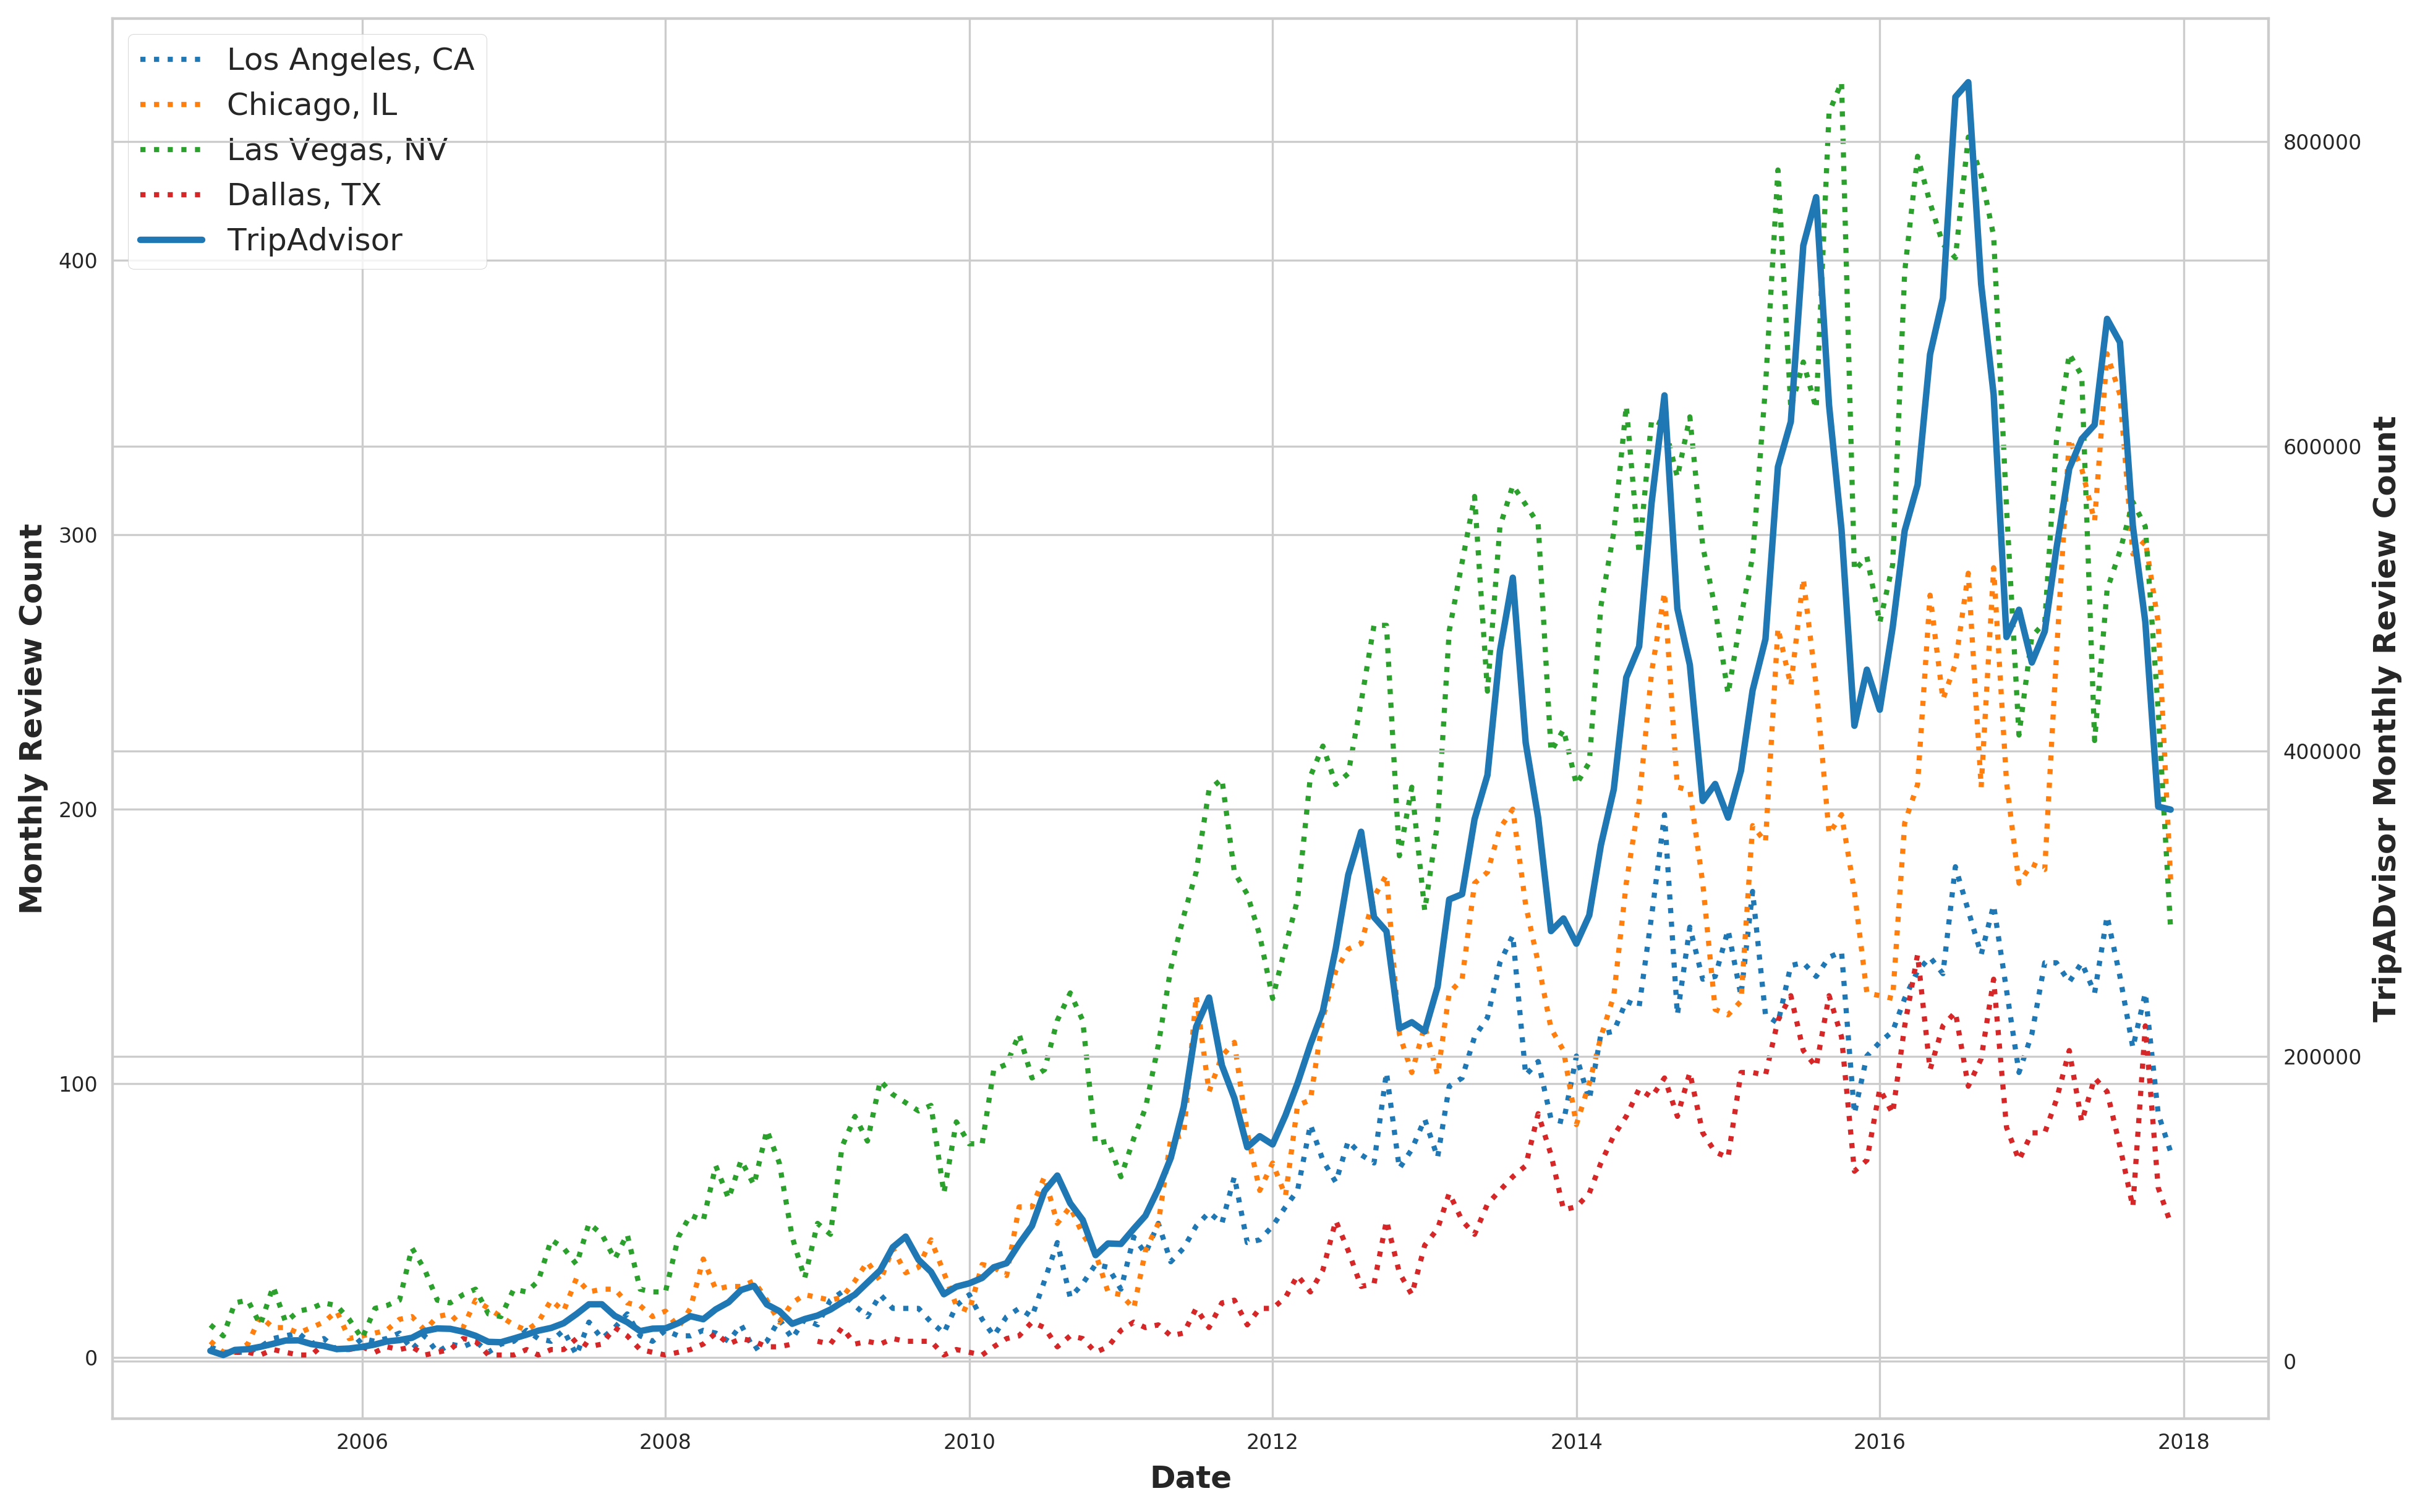
\includegraphics[width=0.8\textwidth,height=\textheight,keepaspectratio]{./Figures/TA_Adoption.png}
% \end{figure}
% \clearpage

 
\begin{figure}[htp]
\caption{EXAMPLES OF ESTIMATED LATENT MEASURES}
 \centering
 \subfloat[LATENT PENETRATION]
 {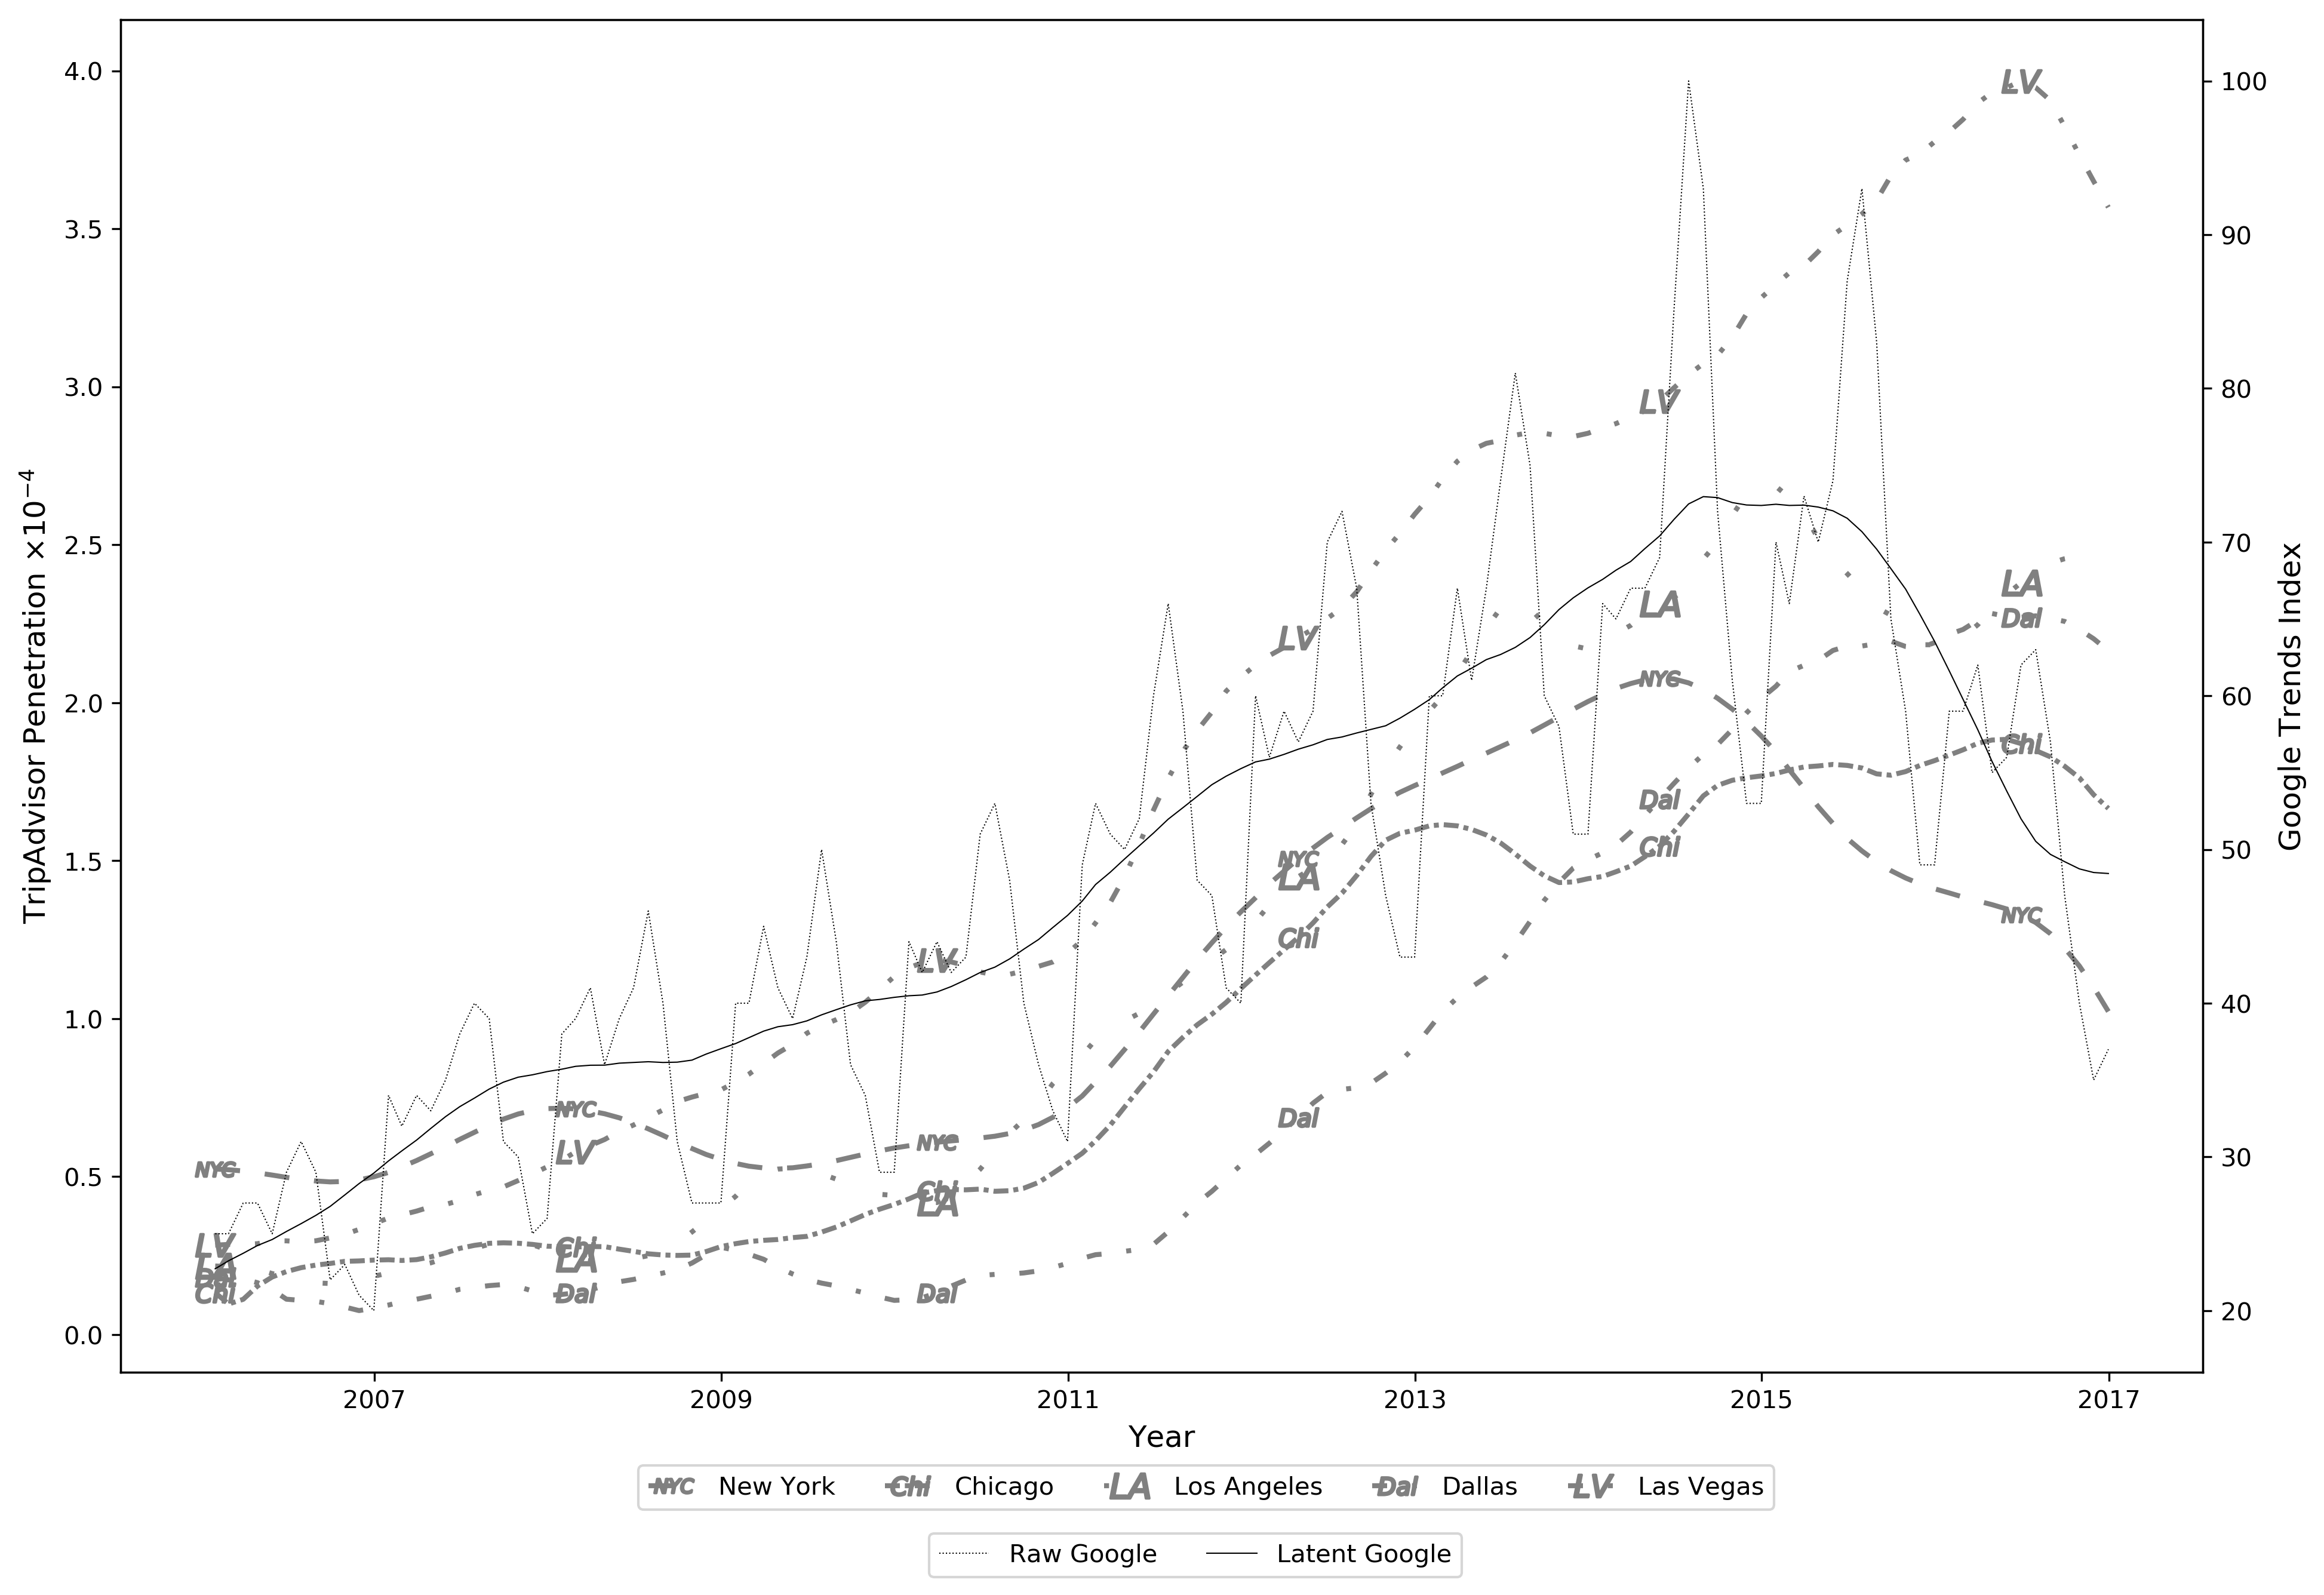
\includegraphics[width=0.5\textwidth,height=\textheight,keepaspectratio]{./Figures/TA_Penetration.png} 
 \label{fig:latentpen} }
 \\
  \subfloat[LATENT QUALITY:Embassy Suites (Memphis, TN)]
  {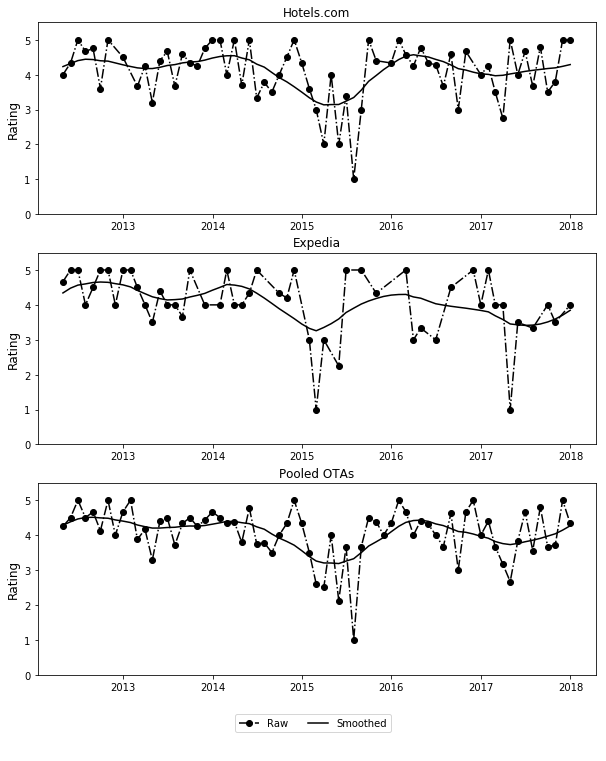
\includegraphics[width=0.5\textwidth,height=\textheight,keepaspectratio]{./Figures/Smoothed_Qual_18987_v2.png} 
  \label{fig:latentqual}}
\end{figure}
 \begin{flushleft}
\small
\textit{Note}. (a) shows TripAdvisor's Penetration (left y-axis) across major US cities over time. The rank order of market penetration changes; Dallas surpasses Chicago and New York. Google Trends Index (right y-axis) documents the Google search results for "TripAdvisor".

% Above is an example of a randomly chosen hotel's raw ratings and latent quality as measured by Hotels.com, Expedia, and pooled OTA ratings. Clearly, raw ratings are noisy while the latent quality trends are smooth. However, prolonged periods of extreme ratings are reflected in movement in latent quality. The takeaway here is that latent quality is not significantly swayed by idiosyncratic changes in measurement noise but it is driven by persistent trends in the measure.  
\end{flushleft}
\clearpage

% \begin{figure}[hp]
% \caption{QUALITY CHANGES DURING RENOVATION EVENTS}
%  \label{fig:renovqual}
%  \centering
%  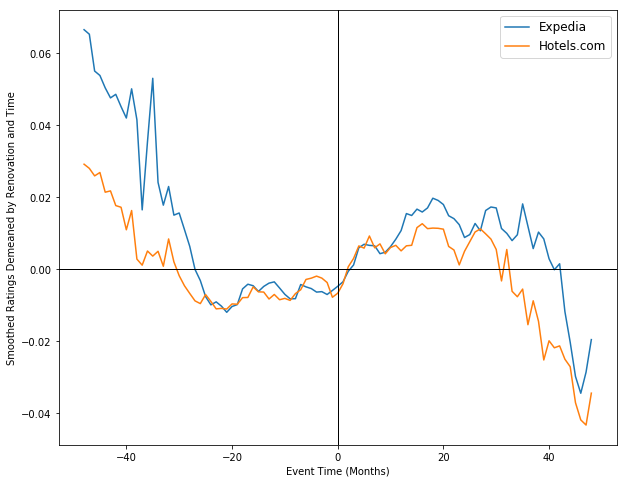
\includegraphics[width=0.8\textwidth,height=\textheight,keepaspectratio]{./Figures/Renovation_Event_dm_ym_event.png}
% \end{figure}
% \clearpage

% \begin{figure}[hp]
% \caption{HOTEL RENOVATION}
%  \label{fig:reno_reg}
%  \centering
%  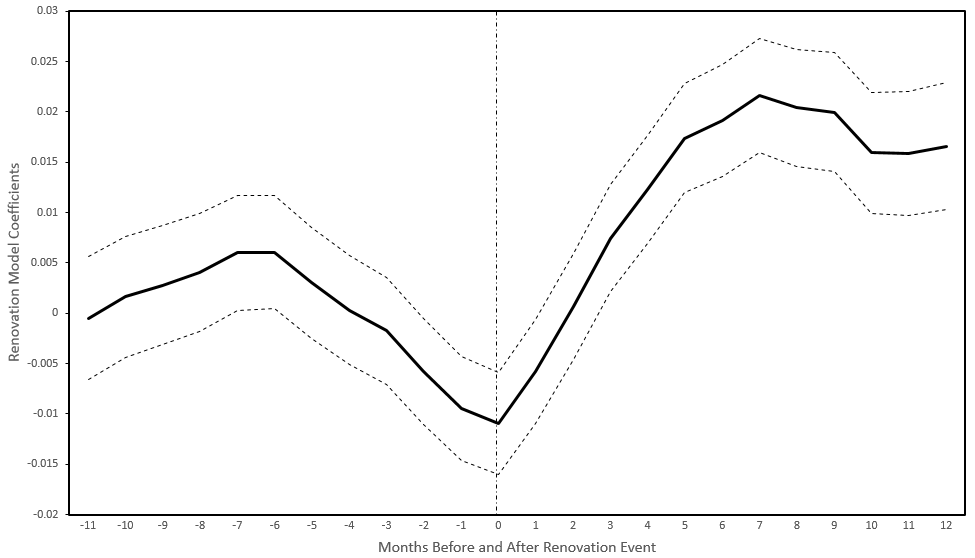
\includegraphics[width=0.8\textwidth,height=\textheight,keepaspectratio]{./Figures/Reno_Reg.png}
% \end{figure}
% \clearpage

\begin{figure}[htp]
\caption{RENOVATION EVENTS}
 \centering
 \subfloat[QUALITY CHANGES DURING RENOVATION EVENTS]
 {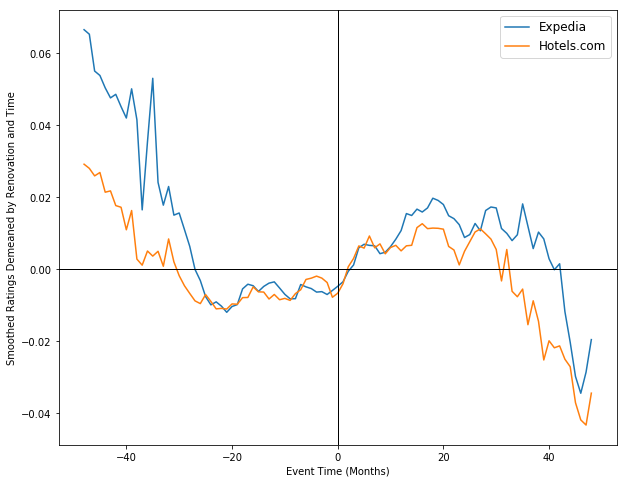
\includegraphics[width=0.8\textwidth,height=\textheight,keepaspectratio]{./Figures/Renovation_Event_dm_ym_event.png} 
 \label{fig:renovqual} }
 \\
  \subfloat[HOTEL RENOVATION]
  {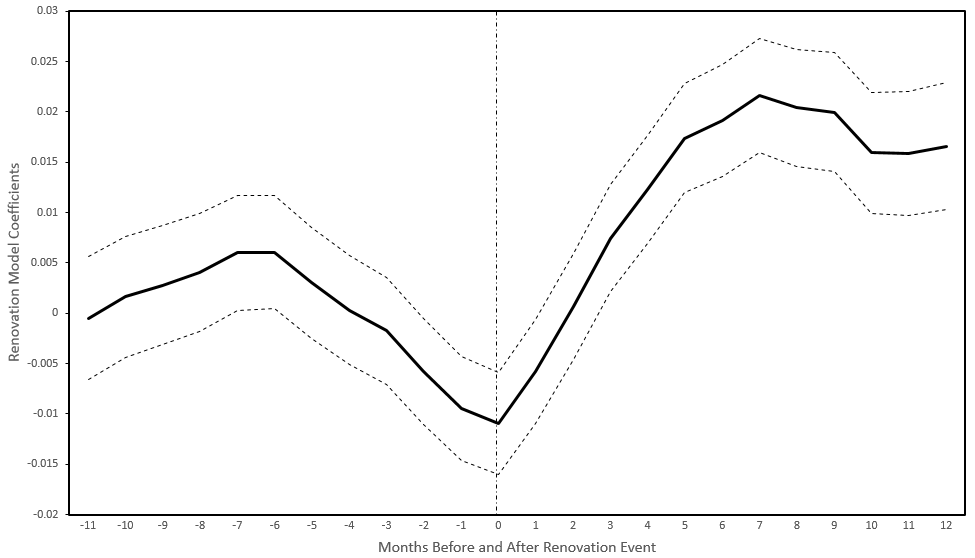
\includegraphics[width=0.8\textwidth,height=\textheight,keepaspectratio]{./Figures/Reno_Reg.png} 
  \label{fig:reno_reg}}
 
 \bigskip 
 \begin{flushleft}
\small
\textit{Note}. (a) demonstrates that, on average, hotels' quality is rapidly decreasing in the 5 years prior to the completion of a renovation and increases as the renovation progresses. The deterioration cycle seems to continue again around 3 years after the renovation. 
\end{flushleft}
  
\end{figure}
\clearpage

\begin{figure}[hp]
\caption{CHAIN ADVANTAGE BY TRIPADVISOR PENETRATION LEVEL}
 \label{fig:modelfree}
 \centering
 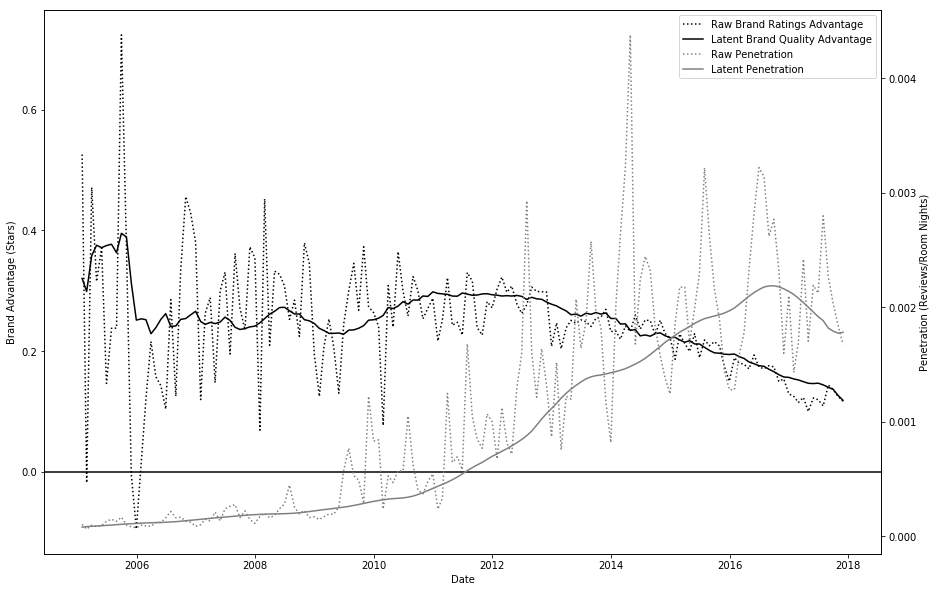
\includegraphics[width=0.8\textwidth,height=\textheight,keepaspectratio]{./Figures/OTA_Brand_v_Chain_v_PenetrationV2.png}
 \begin{flushleft}
\small
\textit{Note}. Brand Quality Advantage (left y-axis: difference between the average of all chains' quality and average of all independents' quality) and TripAdvisor penetration (right y-axis). Brand advantage decreasing as TripAdvisor penetration increases.
\end{flushleft}
\end{figure}
\clearpage

\begin{figure}[hp]
\caption{HDBSCAN AND K-MEANS COMPARISON}
 \centering  
{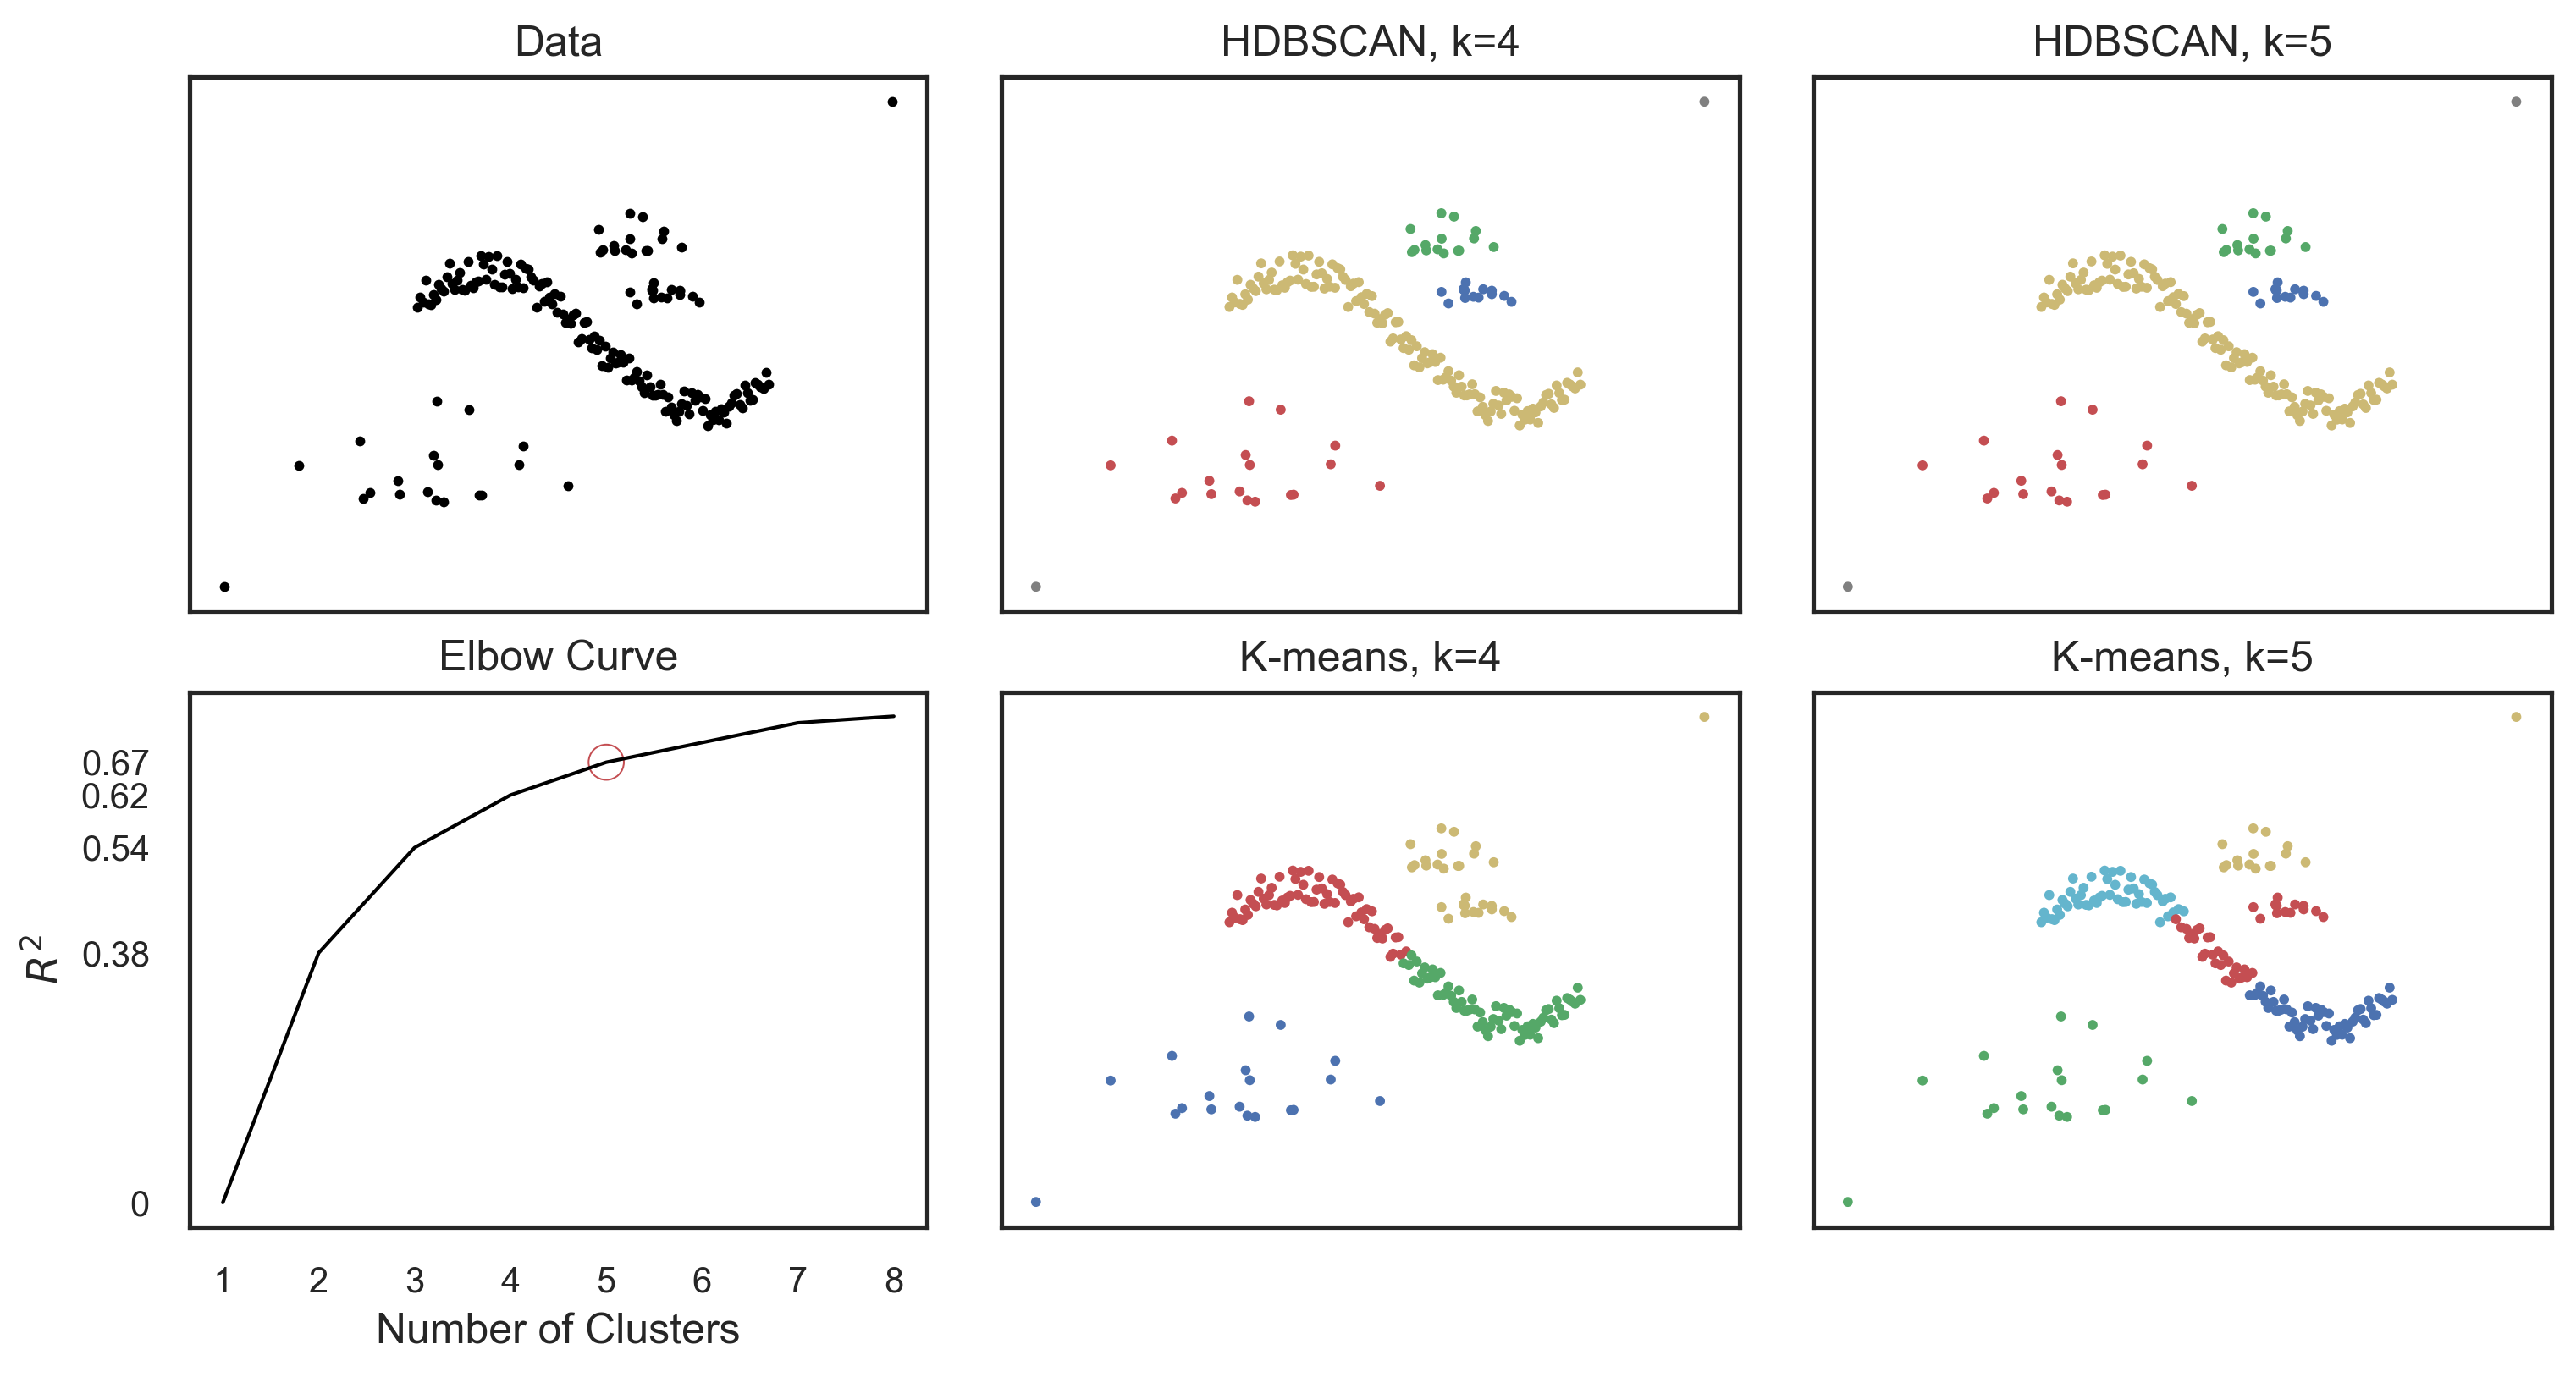
\includegraphics[width=\textwidth,height=\textheight,keepaspectratio]{./Figures/clusters.png} 
\label{fig:cluster}}
\\ 
\begin{flushleft}
\small
\textit{Note}. HDBSCAN is able to detect the visually intuitive clusters while k-means, a common clustering algorithm, struggles, especially with identifying the long cluster following a $sin$ curve.
\end{flushleft}
\end{figure}

\begin{figure}[htp]
 \caption{VISUALIZING EMPIRICAL STRATEGY}
 	 \label{fig:schematic}
\centering
\subfloat[EXAMPLE OF LAS VEGAS MARKETS]{%
  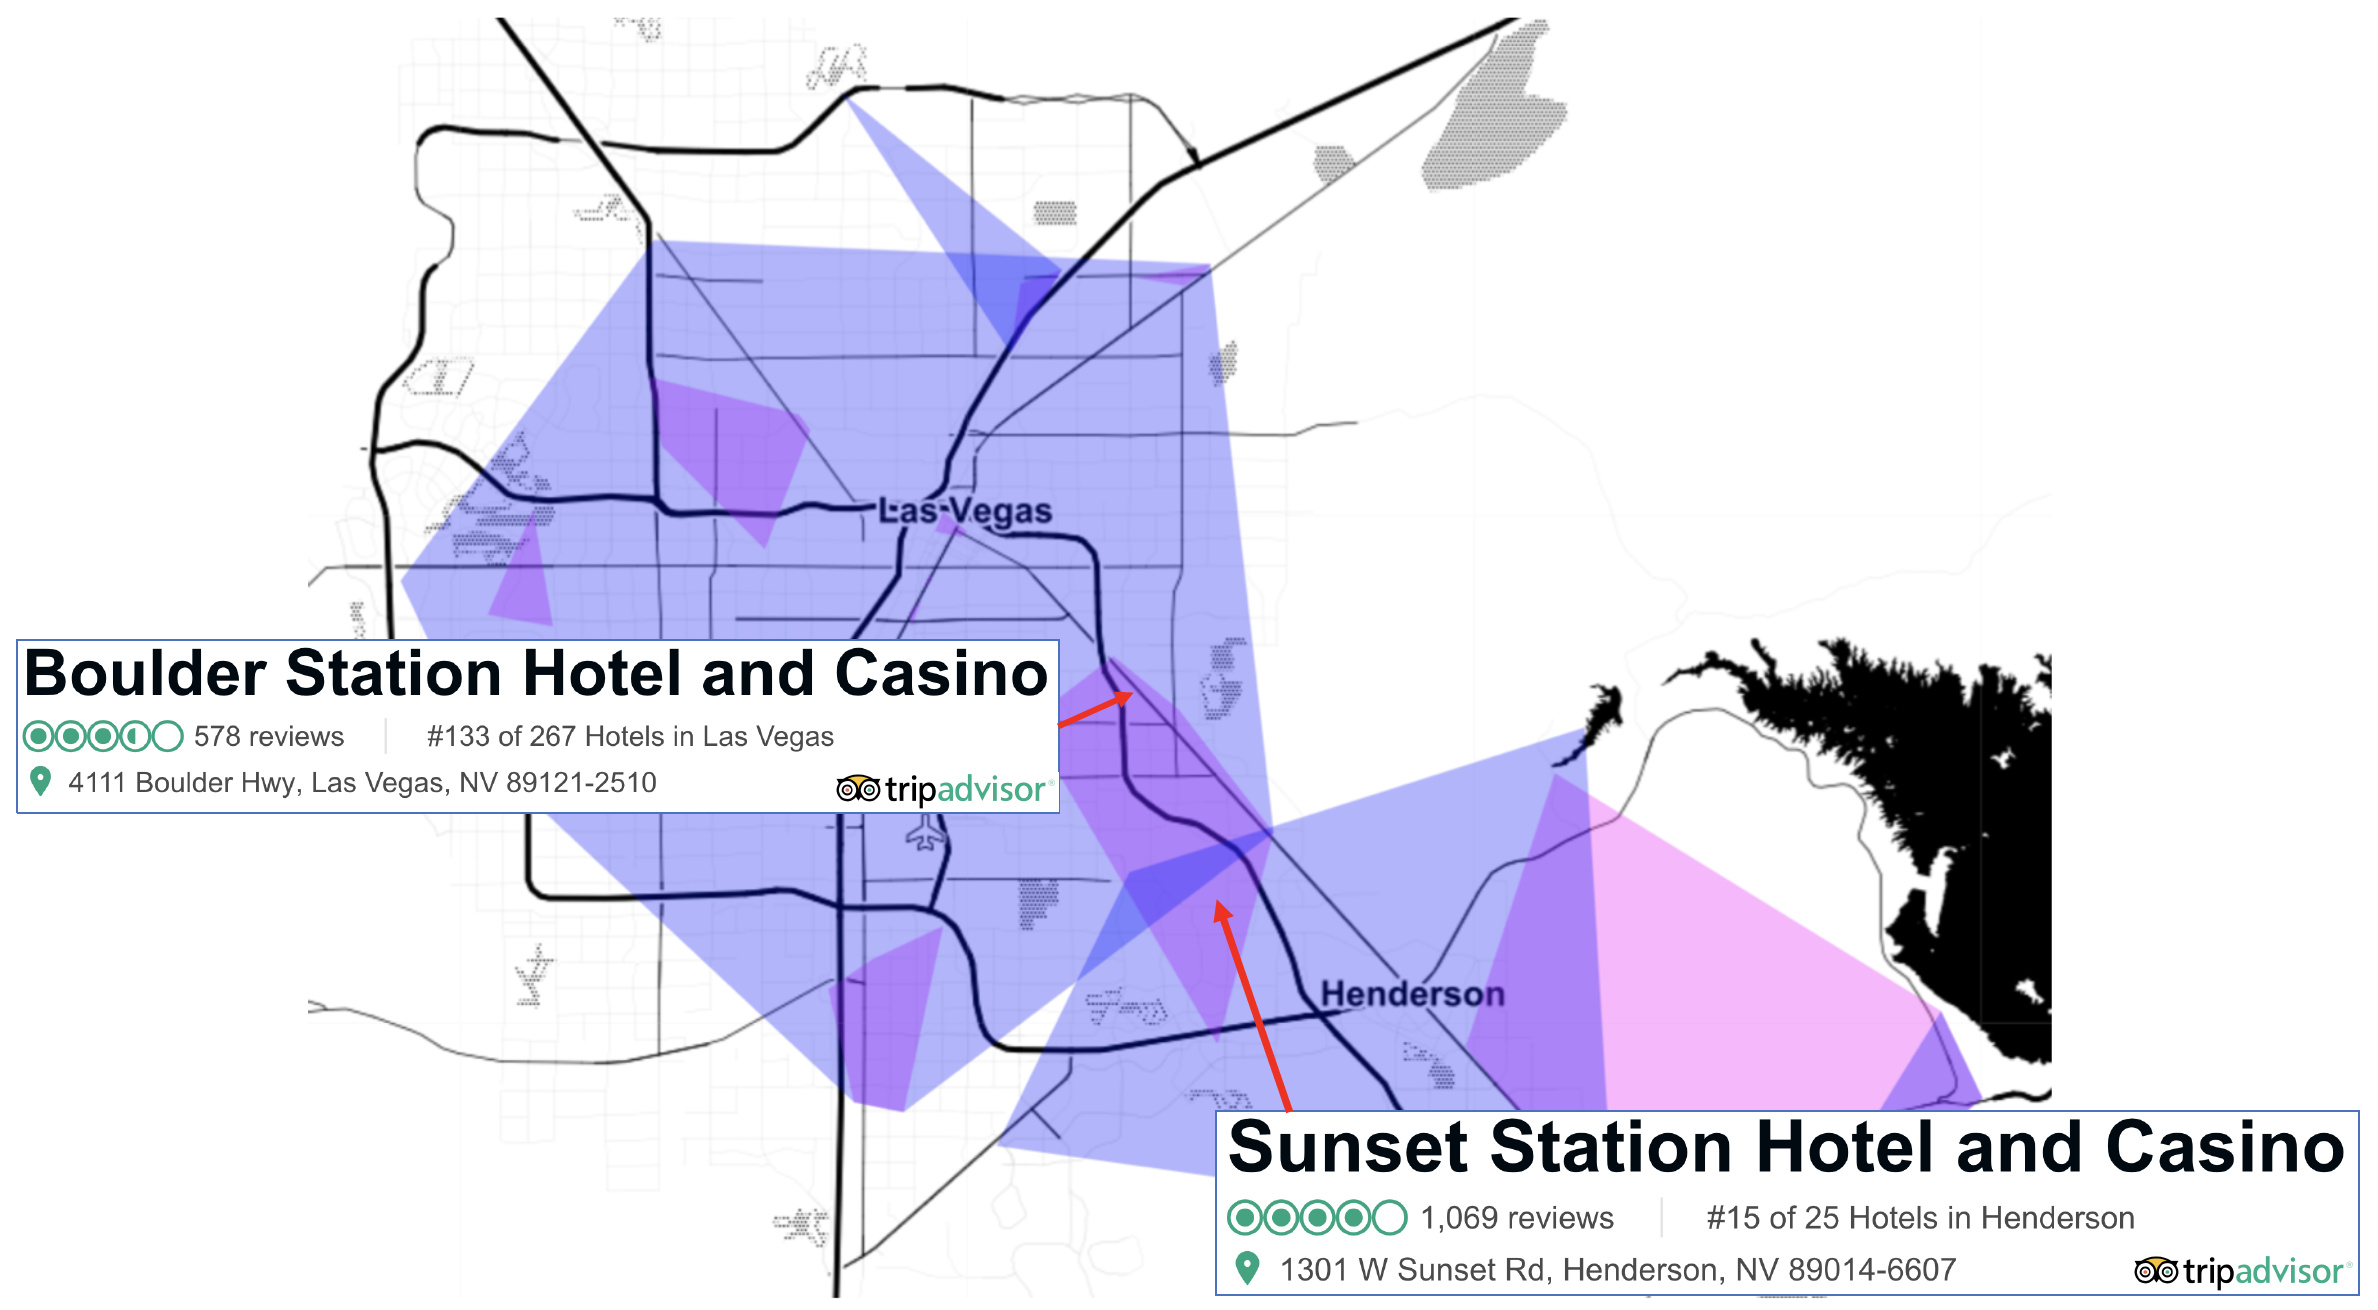
\includegraphics[width=0.6\textwidth,height=\textheight,keepaspectratio]{./Figures/LasVegasMarkets.png}%
    \label{fig:vegas}}%
\\
\subfloat[SCHEMATIC REPRESENTATION OF EMPIRICAL TEST]{%
  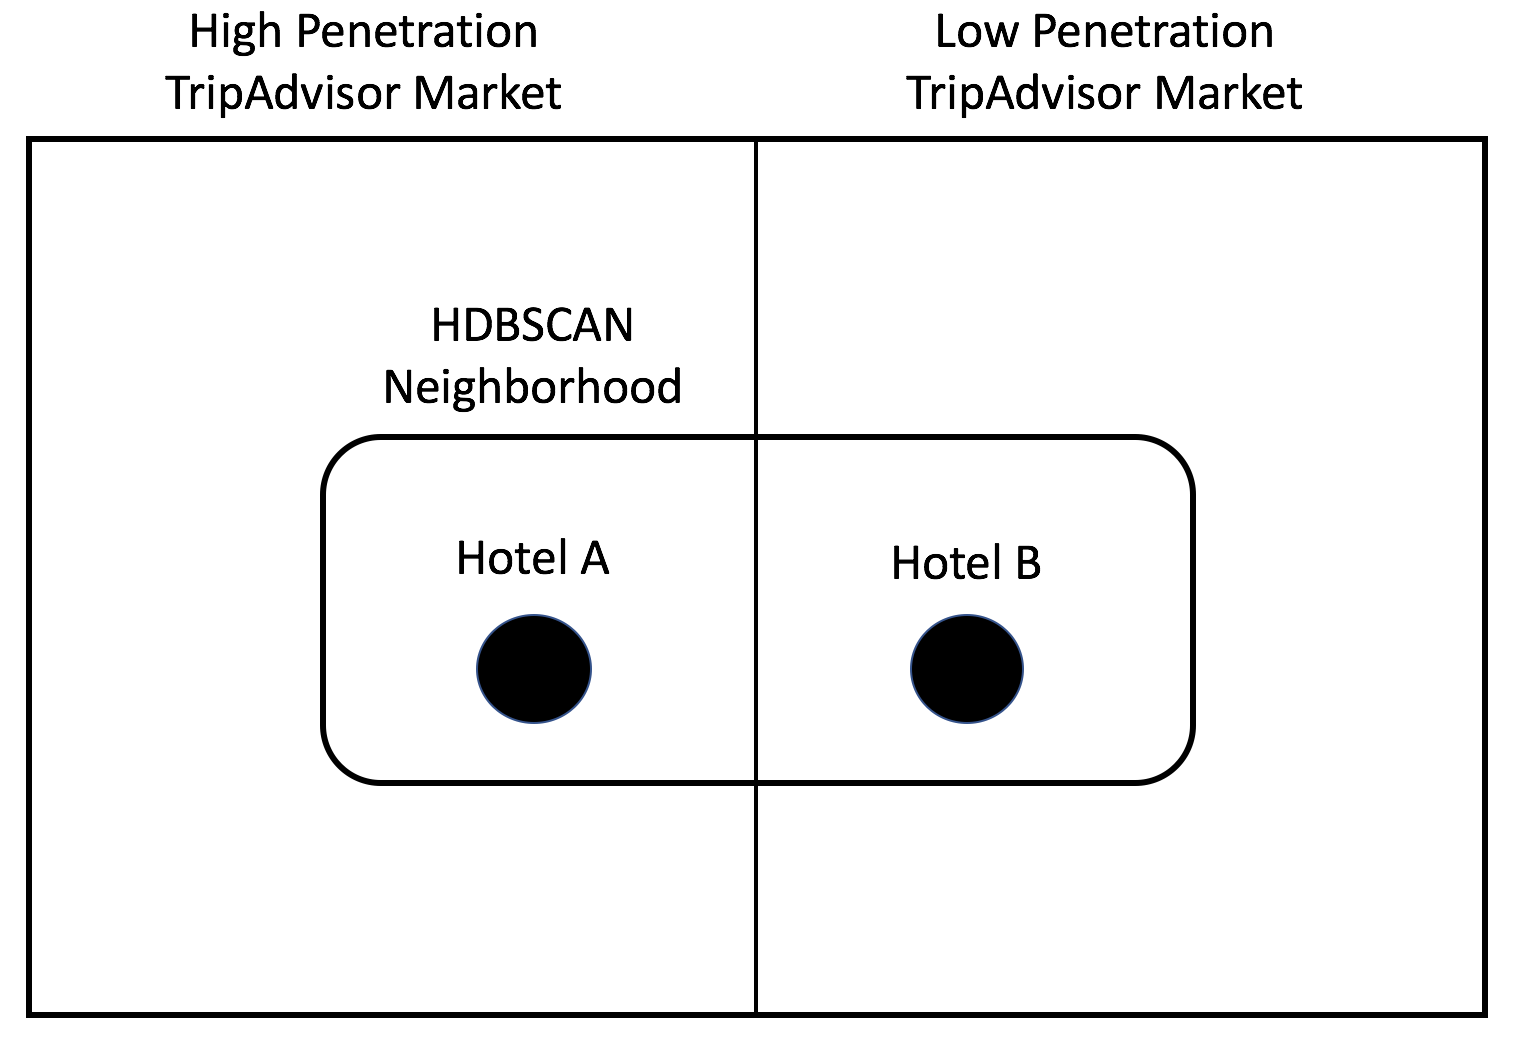
\includegraphics[width=0.6\textwidth,height=\textheight,keepaspectratio]{./Figures/Schematic.png}%
    \label{fig:abmarkets}}
\bigskip 
\begin{flushleft}
\small \textit{Note}. Hotel A and B both belong to the same market cluster based on geographic agglomeration and hotel class, but different TripAdvisor markets and are thus exposed to different volumes of TripAdvisor user scrutiny. We compare the expected quality of hotel A to that of hotel B at a fixed point in time. 
% We operationalize this empirical test with the following high-dimensional fixed
% effect panel regression: 
\end{flushleft}
% \small 
% $\rho_{h,t}=\beta_{1} \pi_{m,t} + \beta_{2} \text{Brand}_{h} + \beta_{3} \pi_{m,t}\times \text{Brand}_{h} + \text{Characteristics}_h\phi + f_{n,t,C}+f_{G}$

\end{figure}
\clearpage

% \begin{figure}[hp]
%  \caption{VISUALIZING EMPIRICAL STRATEGY}
%  	 \label{fig:schematic}
%  \centering
%   \subfigure[EXAMPLE OF LAS VEGAS MARKETS]{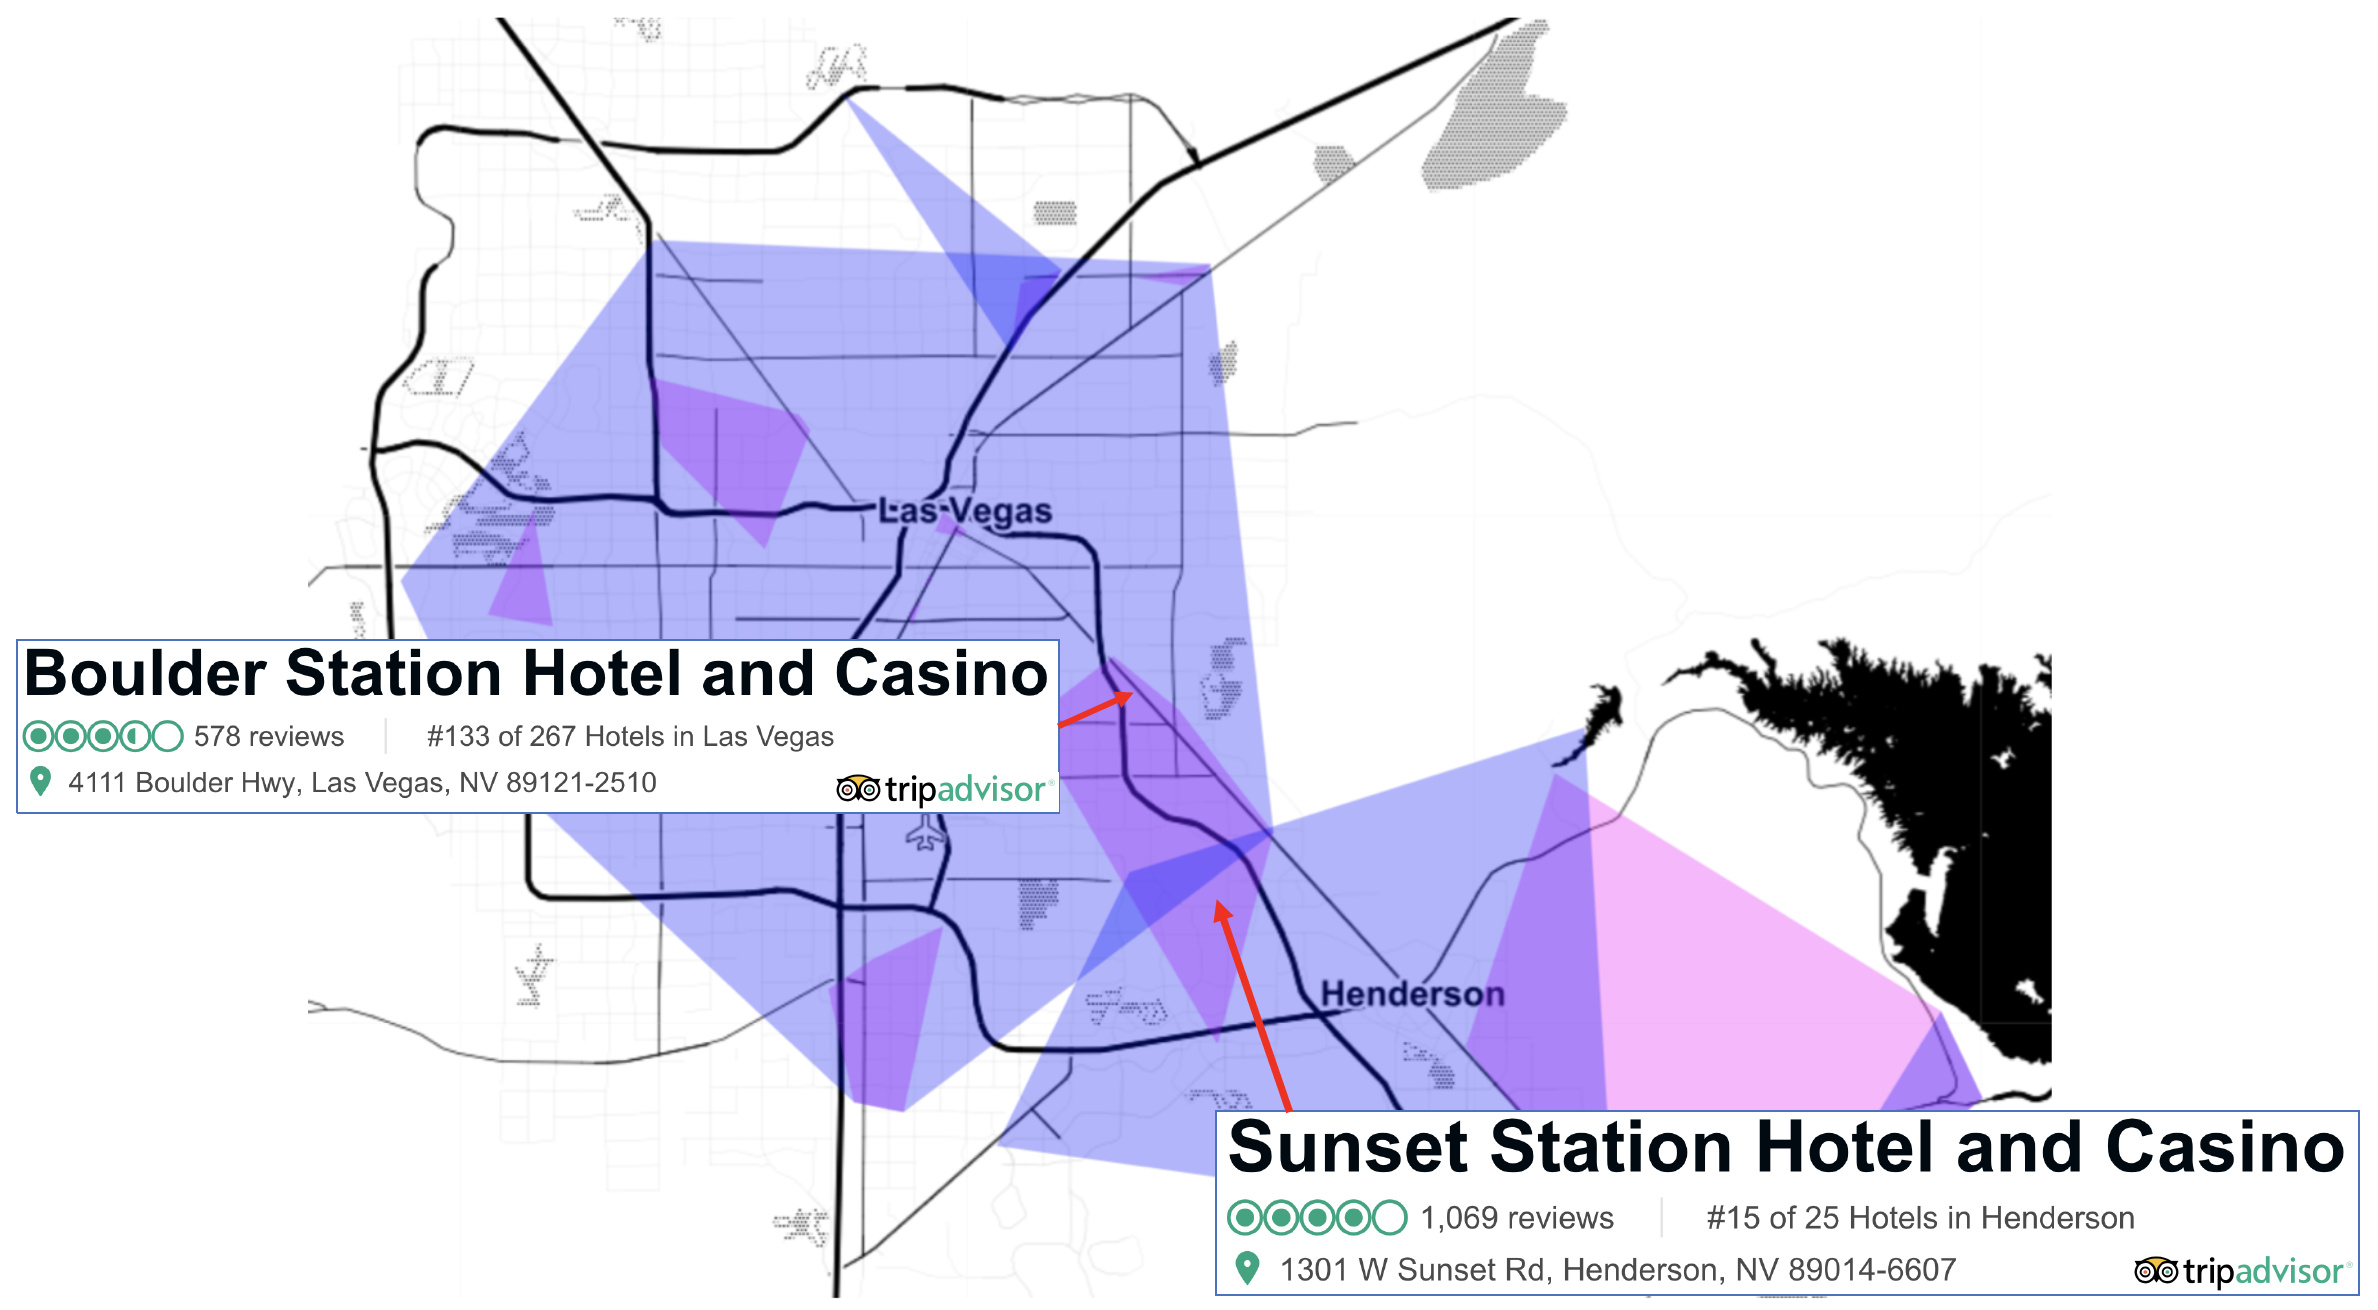
\includegraphics[width=0.8\textwidth,height=\textheight,keepaspectratio]{./Figures/LasVegasMarkets.png} \label{fig:vegas}}
%   \subfigure[SCHEMATIC REPRESENTATION OF EMPIRICAL TEST]{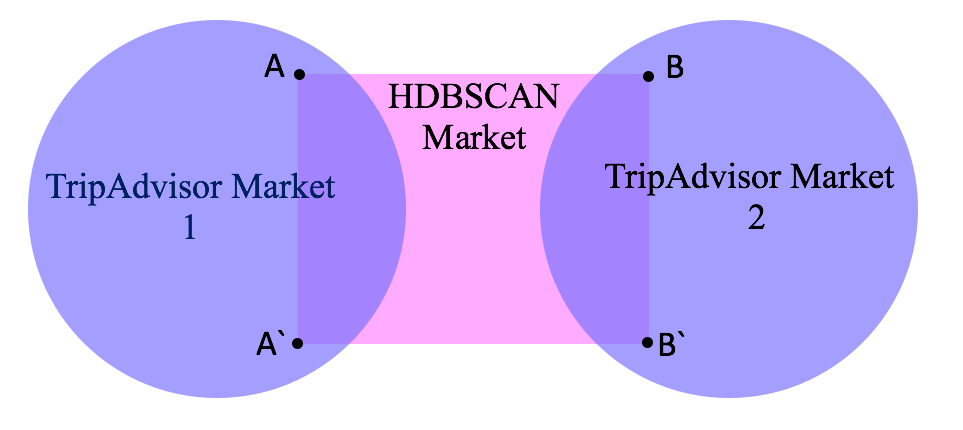
\includegraphics[width=0.8\textwidth,height=\textheight,keepaspectratio]{./Figures/ABMarket.png} \label{fig:abmarkets}}
% \end{figure}
% \clearpage

\begin{figure}[hp]
 \caption{EROSION OF BRAND QUALITY ADVANTAGE}
 \centering
  {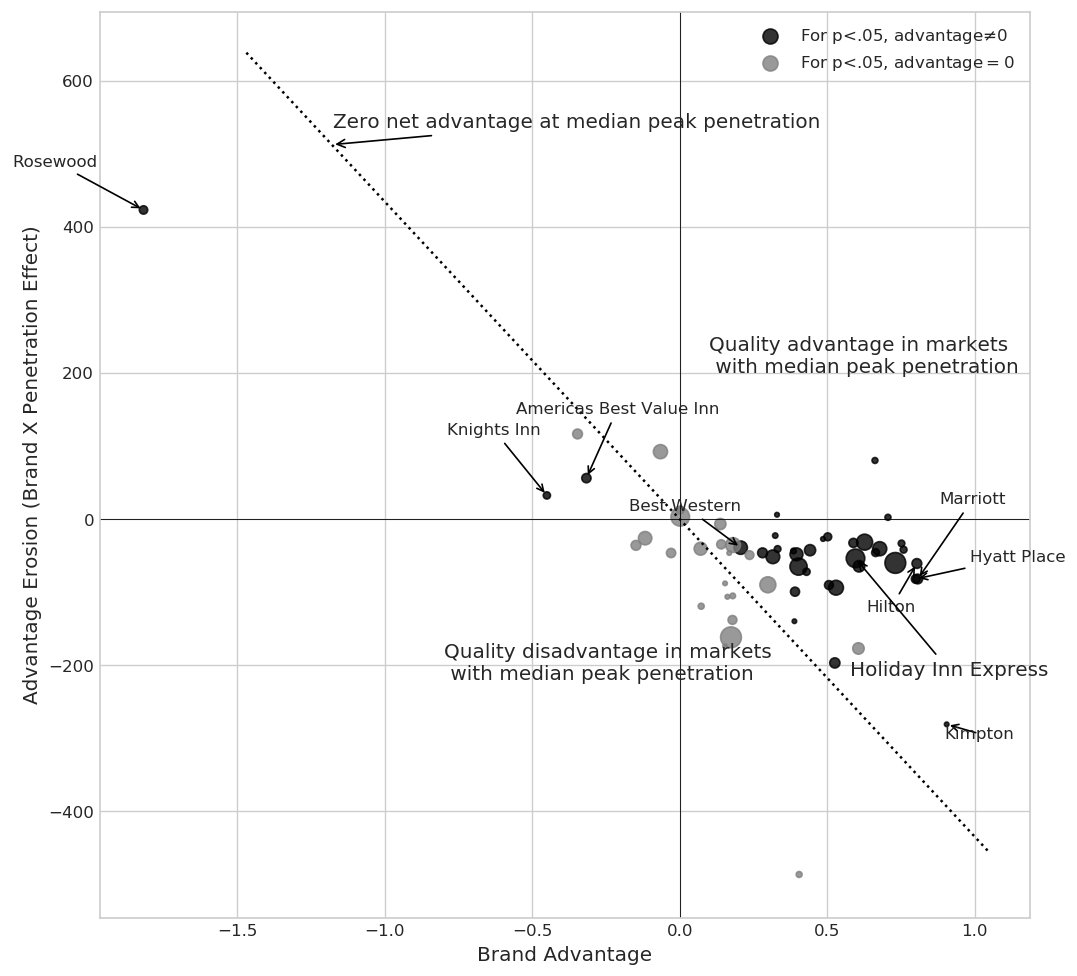
\includegraphics[width=0.8\textwidth,height=\textheight,keepaspectratio]{./Figures/brand_coeff2.png} \label{fig:brandvspenetrate}}
  \\
  \begin{flushleft}
\small \textit{Note}. Brand Advantage (x-axis) versus the Advantage Erosion Effect (brand$\times$penetration effect, y-axis), the black dots are brands with statistically significant coefficients. The region above (below) dotted diagonal line represents brands that hold a quality advantage (disadvantage) in a market with median levels of peak TripAdvisor penetration. The brand's room capacity is represented by the dot's diameter. 
\end{flushleft}
\end{figure}
\clearpage



% Acknowledgments here
\ACKNOWLEDGMENT{%
% Enter the text of acknowledgments here
}% Leave this (end of acknowledgment)


% Appendix here
% Options are (1) APPENDIX (with or without general title) or 
%             (2) APPENDICES (if it has more than one unrelated sections)
% Outcomment the appropriate case if necessary
%
% \begin{APPENDIX}{<Title of the Appendix>}
% \end{APPENDIX}
%
%   or 
%
% \begin{APPENDICES}
% \section{<Title of Section A>}
% \section{<Title of Section B>}
% etc
% \end{APPENDICES}

% References here (outcomment the appropriate case) 

% CASE 1: BiBTeX used to constantly update the references 
%   (while the paper is being written).
\bibliographystyle{informs2014} % outcomment this and next line in Case 1
\bibliography{references.bib} % if more than one, comma separated

% CASE 2: BiBTeX used to generate mypaper.bbl (to be further fine tuned)
%\input{mypaper.bbl} % outcomment this line in Case 2

\end{document}


